\documentclass[12pt, journal, transmag, onecolumn]{IEEEtran}
\usepackage{graphicx}	
\usepackage{tabu}
\usepackage{blindtext}
\usepackage{amssymb}
\usepackage{setspace}
\usepackage{hyperref}
\usepackage{subcaption}
\usepackage{mathtools}
\usepackage{tabularx}
\usepackage{todonotes}
\usepackage{wrapfig}
\usepackage{gensymb}
\usepackage[normalem]{ulem}
\usepackage[final]{pdfpages}
\useunder{\uline}{\ul}{}
\DeclarePairedDelimiter\ceil{\lceil}{\rceil}
\DeclarePairedDelimiter\floor{\lfloor}{\rfloor}
\usepackage{multirow}

\begin{document}


\listoftodos
\clearpage
\spacing{1.2}

\title{Cost Effective Demonstration of Wave-Particle\\ Duality on a Table Top}
\author{\IEEEauthorblockN{Johnny Allain-Labon (JAL), Chong Keat Gea (CKG), Steven Vuong (SV), Georges Ajaka (GA), \\Benji Berczi (BB), Kelvin Fang (KF), Alex Stock (AS), Mohit Motwani (MM)}
\IEEEauthorblockA{Department of Physics and Astronomy, University College London, London WC1E 6BT
\\Board member: Professor Ryan Nichol}
}


\IEEEtitleabstractindextext{
\begin{abstract}

An attempt was made to develop an experimental apparatus and accompanying computer simulation for demonstrating quantum phenomena on a macroscopic scale. This was aimed at functioning as an educational aid for A-level and undergraduate students. The experimental apparatus designed was affordable, easily replicable and successfully demonstrates bouncing droplets on a vibrating liquid surface. The team faced difficulty demonstrating quantum phenomena with the apparatus. The computer simulation developed ran on Java using published mathematical models with simplifying assumptions. Preliminary tests conducted on the simulations suggest that the assumptions used were valid. However, more detailed analysis on the results of the simulation is needed to fully support these assumptions. Lack of time and resources were the primary constrains faced by the team. Future extensions in developing the apparatus and accompanying computer simulation to clearly demonstrate quantum phenomena are proposed. This report provides an outline of work done over the course of this project, including documentation of the prototype and simulation progress, and evaluation of preliminary educational outreach efforts.

\end{abstract}
}

% make the title area
\maketitle
\clearpage
\shipout\null


\section*{Executive Summary}
Our group was tasked with constructing an affordable table-top bouncing oil drop experiment, and to use it to demonstrate some features of quantum mechanics. The experimental demonstration could be augmented with a computer simulation of more advanced quantum features. The simulation could be enhanced by some form of automated statistical analysis of the bouncing oil drops. The direction for our project was left open-ended and up to our discretion. We therefore decided to split the group into two subgroups, one focused on constructing a prototype of the table-top experiment (the prototype group), and another to develop the simulation (the simulation group). Each group was left to independently identify their own measures of success and plan and execute their work loads.

\subsection*{The Prototype Group}
The prototype group was asked to focus on developing the table-top experiment. The aims identified for the prototype group were:
\begin{enumerate}
    \item The setup of the experiment should be affordable and easily replicable.
\item The experiment should exhibit quantum phenomena, including tunnelling and diffraction.
\item The experiment should be an effective teaching tool that is simple and easy to use.
\end{enumerate}

Inspiration for our setup was drawn from the apparatus used in the Veritasium video \cite{Veritasium:2016} and the paper on which it was based. The setup aimed to produce bouncing oil droplets in a petri dish containing silicone oil, driven by a loud speaker. The behaviour of these bouncing oil drops could then be used to demonstrate quantum effects by varying the static depth of oil at each part of the petri dish.

Due to variations in circumstances during experimental procedure, novel adaptations in equipment and methodology were introduced. These include powering the speaker with a Hi-Fi amplifier and replacing silicone oil with diluted washing up liquid. These changes improved visibility, bouncing amplitude and manipulability of the droplets produced. Using diluted washing up liquid instead of silicon oil also significantly reduced the cost of replicating this experiment. The housing for the setup was designed to be easily assembled from pieces of predefined laser cut wood, ensuring easy replicability.  

Footage of the oscillating droplets was captured using a 1000 fps ultra-high-speed camera. By analysing this footage using Adobe AfterEffects, we were able to clearly visualise the ripples and interactions of the droplets and track their movement. By fitting a sinusoidal wave to the vertical displacement of the droplet, we were able to show that the droplet did exhibit simple harmonic motion. 

While our prototype succeeded in observing bouncing droplets, we faced setbacks in trying to demonstrate quantum phenomena, as well as quantifying our data. This was attributed to time restrictions, as well as the numerous variables unaccounted for; such as temperature and droplet size. We have proposed modifications in methodology and in equipment for future experiments to demonstrate quantum phenomena, as well as to control some of the unaccounted-for variables.

Demonstrations to a class of year 12 A-Level Physics students provided optimistic responses as to the efficacy of our prototype as a teaching tool. Students participating in our demonstrations felt more engaged and curious, and displayed better understanding of quantum phenomena. Teachers present at the demonstration also gave positive feedback on the experiment. 
We have also planned future extensions for what was accomplished by this subgroup. First, we would like to produce an educational report aimed at winning an award by the STFC for small projects. Next, we would also like to create an apparatus that could demonstrate quantum phenomena better. To account for the probabilistic nature of QM, future setups will need to be able to repeat trials of the same system parameters over an extended period of time.

\subsection*{The Simulation Group}
The simulation group was tasked to focus on developing the computer generated graphical representation. The aims were:

\begin{enumerate}
    \item The simulation should operate with an interactive, simple graphics user interface (GUI).
    \item The simulation should be able to display demonstrations of bouncing
droplets in real time.
    \item The simulation should be able to modify any system parameter.
\item The simulation should be able to demonstrate quantum phenomena and perform statistical analysis of the bouncing droplet. 
\end{enumerate}

Inspiration for our simulations was drawn from the work by the DotWave group \cite{dotwave}. Code used in the video simulations published by the DotWave group was not publicly accessible. Hence, it was necessary for us to build the simulation from scratch. The aim of the computer suitable simulation was to have it be performed by a program with the entire mathematical model hard coded in. The program would therefore only require system parameters and start conditions input to perform and display the simulation.
In our simulations, mathematical models published by \cite{oza2013trajectory} and \cite{brady2014bouncing}, along with a few simplifying assumptions were used. Initial tests were conducted on the mathematical models in python, Matlab and Java. While python and Matlab had native modules to display graphical data in 3-D, the calculation rates were too slow to be suitable for live demonstrations. Java, however, proved to be extremely efficient at performing calculations but slow in generating and displaying frames. 

Attempts to exploit the efficient processing power of Java and the native display modules of Matlab was made by interfacing the two programming languages. Failure to produce such an interface was due to our lack of computing expertise. It was thus concluded that we did not possess sufficient expertise and processing power to produce a program that could display the simulations live.

Java, being the most efficient and flexible programming language tested, was used in further developments. The video visualising each simulation was produced by using the Java code to output each frame as a png file and stitching them together using a third-party software. The Java code also outputs the position and velocity data of the droplets simulated at each timestep into a csv file. The data collected was later used for further analysis. System parameters in all simulations performed were hard coded using values provided by the DotWave group. A simple modification to the Java files would enable it to accept any input values as system parameters.

Simulations at various memory values were conducted. The results of the simulation match the theoretical prediction that the simulated bouncing droplet would only enter the walking state in the high memory regime. This provided evidence that supports the validity of the mathematical model and its accompanying simplifying assumptions used in our program.

Preliminary tests were conducted to simulate the effect of two droplets initiated next to each other and the behaviour of the droplet upon introduction of a fully reflective wall. Due to time constraints we were unable to develop the code further to demonstrate quantum phenomena, nor perform statistical analysis of the bouncing droplet. 

\clearpage

\clearpage
\setcounter{tocdepth}{2}

\tableofcontents
\clearpage

\section{Group Organisation (MM)}
\subsection{Assigned Roles}
Central to any successful project is effective, efficient division of labour, in order to ensure that all necessary tasks are accomplished on time, and to a high standard. In order to accomplish this, it was decided that the project, having two clear avenues to follow, required the creation of two subgroups: an experimental group and a simulation group. The former were to handle the creation of the apparatus, experimentation and preliminary outreach efforts, whilst the latter were to handle the creation of a simulation that could effectively display these physical phenomena. Of course, due to the varied nature of the project and constantly fluctuating workloads, several changes were made to personnel roles over the course of the project. Therefore, a brief outline of each group member's responsibilities is given as follows:

\textbf{Mohit Motwani} (MM) initially took responsibility for the final written report and has seen the whole report through to the end, writing both the intro and theory. Johnny also jumped aboard at a later stage to assist with the editing. Alongside this, Mohit also worked on the experimental prototype during the first half of term whilst equipment was being gathered. Specifically, he researched into slow-motion photography for tracking droplet motion as well as recorded meeting minutes. Following the subdivision, Mohit liaised with Mark Fuller and Johnny to create a lesson plan and worked with Benji to outline the objectives for outreach. The lesson plan was eventually executed at Chesham Grammar School in a pilot outreach lesson with Johnny and Steven.

\textbf{Johnny Allain-Labon} (JAL) took responsibility as group secretary, communicating with the board member and the group as well as typing up minutes. Having done PHAS3459, Johnny investigated the animation aspect of wave-functions in python and Java, coding basic generation of frames used by the simulation group as well as helping report on work accomplished. Following this, Johnny co-created and eventually delivered a lesson plan for Chesham Grammar School, leading up with the results of the outreach effort. Finally Johnny held joint responsibility with Mohit in writing and editing the written report and structured and made the typeset for the poster.

\textbf{Chong Keat Gea} (CKG) took responsibility as chair, in doing so produced meeting agendas, managed group dynamics and tracked time management ensuring that simulation and prototype groups were progressing at a steady rate. Additionally Gea helped distribute workload so team members contributed equally by conducting ‘health checkups’ at every meeting, delegating additional roles to team members who felt they were not contributing enough. Gea also interacted with staff at the Institute of Making and developed the prototype plywood housing, also assisting with soldering and wiring of the initial prototype. Upon moving to the simulation team, Gea developed a random point generator from a probability density function, using the math in the Matlab file in Java to perform simulation tests and analysis with multiple droplet simulations.

\textbf{Steven Vuong} (SV) initially wrote a summary of the theory and research material provided as a prompt by the board member before taking responsibility as lead of prototype group. Initially with Gea, Benji, Kelvin and Mohit, Steven co-created the first prototype and managed to obtain access to recording equipment as well as other devices and expertise from various other UCL departments. Eventually Steven and Kelvin in the prototype sub-group worked in labs to make and record observations into bouncing droplets and wrote transcripts of lab sessions throughout. Steven also went into Chesham Grammar with Mohit and Johnny to aid in outreach and helped to gauge feedback for improvement before finally assisting in writing the experimental section of the final report.

\textbf{Georges Ajaka} (GA) took lead as simulation group, organising simulation group meetings and reported progress to the rest of the group in weekly meetings. Georges initially researched suitable theories which could be applied to simulation, with this he created an initial Java graphics interface where he made velocity dependent colouring scale for trajectory lines implemented on a random point generator. Furthermore, Georges worked on integrating MATLAB and Java code before assisting in writing the simulation section of the final report. Georges also made a final repository for all the code.

\textbf{Benji Berczi} (BB) started on the prototype group and researched equipment lists which were used to build the first working prototype which he also took part of. Benji was then responsible for writing the peer-assessment of the other group’s meeting and wrote their critical assessment. Alongside this, Benji collaborated with Mohit and took the lead in writing a business proposal aimed at winning an STFC run award in developing the educational aspect of the prototype and also explored commercialisation possibilities. Benji also worked on the final poster.

\textbf{Kelvin Fang} (KF) initially further developed research material and found papers surrounding the topic which were used by the simulation group. Kelvin also took initiative of coming up with a lab script for our entire lab script which he saw through and experimental log template which were used to record experimental observations. Kelvin also booked meeting rooms. Kelvin supplied various apparatus and worked with Steven, Gea and Benji to put together the apparatus. Eventually partnering with Steven to carry out experimentation, video capture and analysis. As Kelvin had access to Adobe AfterEffects, he conducted video processing, photo generation and motion tracking to reveal sinusoidal motion verifying pilot wave theory of our bouncing droplet. Finally Kelvin assisted in writing out the experimental methods section for the final report.

\textbf{Alex Stock} (AS) conducted research to find suitable theories which could be applied for simulation. As Alex had prior experience with MATLAB, he formulated the basis for the final model which was eventually ported into java. Alex wrote this whilst the rest of the simulation group simultaneously attempted to create a bouncing droplet into java. Alex then took responsibility for his code and followed it through, assisting in implementing his mode into java and writing the simulation section of the report. Finally, Alex assisted in writing the theory section of the final report.


\subsection{Budget}
To carry out this project, we received an initial sum of \pounds200. This was to include all manufacturing costs, alongside the cost of poster printing. It was an ambitious limit, considering previous investigations of a similar similar were carried out in full-fledged research laboratories, with the corresponding resources. Nevertheless, some of the initial objectives were accomplished, with a substantial sum being left over at the summation of \todo{insert final sum left here before final print} of the project. The full expenditure details are given in Table \ref{table:budget}. 

\bigskip                    
\begin{table}
\centering
\begin{tabular}{|c|c|c|}
\hline
&\textbf{Income}& \textbf{Expenditure}\\
\hline
\textbf{Initial budget}& \pounds200&  \\
\textbf{Plywood}& &\pounds3.00  \\
\textbf{ELEGIANT amplifier}& &\pounds12.99  \\
\textbf{Foldback clips}& &\pounds3.00  \\
\textbf{Photron high speed camera rental x2}& &\pounds50.00  \\
\textbf{Outreach travel expenses}& &\pounds24.00  \\
\textbf{Sharelatex account}& &\pounds7.20  \\
\textbf{Draft report print costs}& &\pounds1.85  \\
\textbf{LED lights}& &\pounds6.99  \\
\textbf{Final report and binding}& &\pounds TBC  \\
\textbf{Amplifier power supply}& &\pounds6.99  \\
\textbf{Poster}& &\pounds 40.00  \\
\hline
\multicolumn{3}{|c|}{\textbf{Total expenditure \pounds161.86}}\\
\hline
\multicolumn{3}{|c|}{\textbf{Sum remaining \pounds38.14}}\\
\hline
\end{tabular}
\caption{A summary of the expenses endured over the course of this project. Values for both the money remaining and total spent are given.}
\label{table:budget}
\end{table}
\todo{REPORT PRINTING COSTS}

\subsection{Communication and Administration}
In order to keep both teams updated on group progress overall, and to be able to appropriate specific skills of group members, frequent meetings were in order. Weekly meetings were held, occasionally with the board member present, in order to track progress on a week-by-week basis, and to keep on top of approaching deadlines. Prior to each meeting, the group chair produced an agenda, which acted as a framework for the meeting. Meetings were recorded via minutes, made by the group secretary. These were published online, to give all members a clear outline of responsibilities for the forthcoming week. As this project required group access to a large amount of shared material, a Google Drive folder was set up and organised into clear sub-folders. This was made available to all group members from the start. Group and sub-group communication was handled via Facebook Messenger, with important links pinned on a Facebook group, in order to ensure that no important links were lost in chat. 

Sub groups met once a week to discuss their work further. The experimental team, before splitting to form an educational team, met more frequently to carry out lab work. The simulation team coordinated their efforts through GitHub, which allowed them to sync their work, while also acting as a fail-safe in case of a loss of local files. The prototype group used Google drive to share resources. 
The report was written using ShareLaTeX, an online LaTeX processing tool that allowed for collaborative access, for changes to be tracked and for comments to be made. A template was utilised to make the poster on ShareLaTeX as well. 

\subsection{Group Dynamics}
Overall, there were no issues with group dynamics. Meetings were held frequently, with regular attendance from all members. All members contributed equally, with responsibilities being shared and taken on in a concientou 
\clearpage

\section{Introduction (MM)}
An age-old and much investigated field of research in science has been the nature of light. For centuries, scientists have endeavoured to understand its nature and fundamental properties. At the turn of the 20th century, light was widely believed to behave as a wave, but the discovery of phenomena such as the photoelectric effect called this theory into question. Eventually, it was agreed that light exhibited both wave-like and particle-like behaviour, a phenomenon known as wave-particle duality. The interpretation of this quantum mechanical behaviour, however, is still open to debate.

The commonly accepted interpretation, known as the Copenhagen Interpretation, was first proposed by Niels Bohr and Werner Heisenberg in 1927. It pushed forward the idea that a physical system would only have definite properties upon measurement; prior to measurement it was only possible to measure probabilities of obtaining a given measurement. An alternative interpretation, the De Broglie-Bohm theory, was pushed forwards in 1952. It is deterministic in nature: it claims that even prior to observation there exists a driving equation or `pilot wave' whose properties determine measurements. In 2005, research suggested \cite{couder} that droplets bouncing on a surface could display quantum mechanical behaviour as proposed by pilot wave theory. Indeed, this macroscopic system was a remarkably good analogy for the pilot wave theory; waves induced by a driving droplet quite closely match a driving wave-equation determining the results of measurements. 
\subsection{Aims}\todo{check to see if matches summary}
To this end, the purpose of this project was to develop a cost-effective table top version of the experiment used by \textit{Couder et al.}, demonstrating the various different behaviours of bouncing droplets. Such motion could include simple oscillations, motion parallel to the liquid surface and double slit diffraction of droplet generated waves. It was intended to be paired with a computer based visualisation that can display effects outside the bounds of this apparatus. The overarching goal was to develop a prototype that can be used for outreach purposes, allowing  students to the grasp the non-intuitive nature of quantum mechanics. 

\subsection{Objectives}
The above aims raised the following core project objectives: 
\begin{enumerate}
   \item Development of table top apparatus: 
   \begin{enumerate}
     \item To create a working prototype capable of displaying basic  motion, such as bouncing and walking droplets.
     \item To obtain high speed cameras capable of recording droplet motion
     \item To further improve the prototype, and demonstrate multiple droplet motion (such as droplets repelling and coalescing) and phenomena such as double slit diffraction
    \end{enumerate}
   \item Development of an in-depth simulation:
   \begin{enumerate}
    \item To identify a suitable programming language for simulation purposes
     \item To implement required code in chosen language in order to display droplet motion.
     \item To extend the capabilities of the program in order to cover aspects of quantum mechanics not displayable by the experimental apparatus. Such effects may include double slit diffraction and tunnelling effects, where the droplet escapes through the barrier of a potential well.
    \end{enumerate}
    \item Creating an iteration of the initial prototype usable in college/undergraduate courses as a demonstration tool.  
   \begin{enumerate}
     \item To create a standalone version of the simulation program.
     \item To create a simple to use version of the experimental. apparatus, for third-party users.
     \item To write a business plan for implementation in future.
     \item To explore the possibility of testing the apparatus with undergraduates and A-level students.
    \end{enumerate}
\end{enumerate}

\clearpage

\section{Theory (MM, AS)}\label{theory}
\subsection{Droplet motion}
This investigation focuses on the motion of moving droplets on a liquid surface. In 1978 it was reported \cite{Walker} that droplets vibrating at a certain frequency upon a soap-solution surface would not immediately coalesce, but could maintain motion for up to 18 minutes. Couder \textit{et al.} further researched this phenomenon in 2005 \cite{couder}. Using a silicon oil surface (with no soap-substrate) they discovered that it was possible to create a   an oscillating droplet at certain frequencies, and even walking droplets that moved parallel to the surface. 
The walking droplets were created by simply vibrating the liquid surface vertically at a frequency determined by: (\ref{eq:bouncing regime condition}):

\begin{equation} \label{eq:bouncing regime condition}
\frac{\gamma_{m}^{B}}{g}\approx 1
\end{equation}
$g$ is the acceleration due to gravity, $\gamma_{m}^{B}$ is the specific value of co-efficient $\gamma_{m}$ of (\ref{eq:vertical acceleration}).


\begin{equation} \label{eq:vertical acceleration}
\gamma=\gamma_{m}cos(2 \pi f_0t) 
\end{equation}

(\ref{eq:vertical acceleration}) determines $\gamma$, which is the vertical acceleration of the fluid, $f_0$ is the driving frequency of the liquid and $t$ is time. The droplets bounce due to a remarkably simple mechanism. Upon collision of a droplet with the liquid, there exists a thin layer of air trapped between the two surfaces. Normally, the droplet will coalesce with a surface in a matter of seconds, as this air is forced away. However above a threshold value of $\gamma_{m}$, the droplet will instead bounce, as the air film retains its integrity, forcing the droplet upwards. By specifying a threshold vertical acceleration, it is also ensured that the air film will have a chance to replenish after each subsequent bounce, allowing the motion to be periodic over a large period of time. The regimes in which different types of motion occur are described in Figure \ref{regimes}.

\begin{figure}[ht]
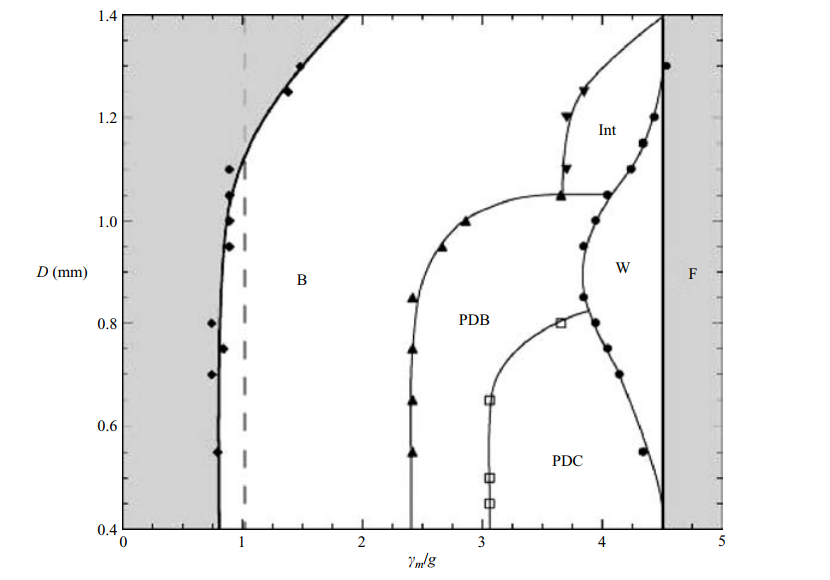
\includegraphics[width=12cm]{theory/regime}
\centering
\caption{A graph of droplet diameter against $\frac{\gamma_{m}}{g}$ for an oscillating droplet in a vibrating liquid. It illustrates the different vertical acceleration regimes: Bouncing (B), Walking (W), Faraday instability (F), Period Doubling (PDB), transition from Periodic to chaotic behaviour (PDC)  and Intermittent behaviour (Int).}
\centering
\label{regimes}
\end{figure}

Furthermore, droplets can also exhibit motion parallel to the droplet surface. Such droplets are labelled walkers, and like bouncing droplets, they exist in a certain $\frac{\gamma_{m}}{g}$ regime, just below the onset of the Faraday instability. The Faraday instability is defined as the point at which a surface becomes spontaneously wavy. Just before its onset, a bouncing droplet has a period of motion twice that of its driving oscillation. It thus generates a damped travelling Faraday wave at each bounce, where Faraday waves are standing waves generated by a vibrating liquid. The subsequent landing then occurs on the reverse slope of this previously generated Faraday wave. This landing generates another travelling Faraday wave, and causes the droplet to perform a parabolic bounce, causing motion parallel to the surface. An intuitive way to understand this motion is to imagine jumping on a trampoline. Each time you land on the trampoline, a wave is generated. If you land again anywhere but at the centre of this wave, you spring off again, and your motion has a slight horizontal component, allowing you to travel around the trampoline. As the wave you generate when landing travels, you constantly land on its side, therefore there is a constant horizontal motion, allowing you to 'walk' around the trampoline. This motion is illustrated in Figure \ref{walker}. 

\begin{figure}[ht]
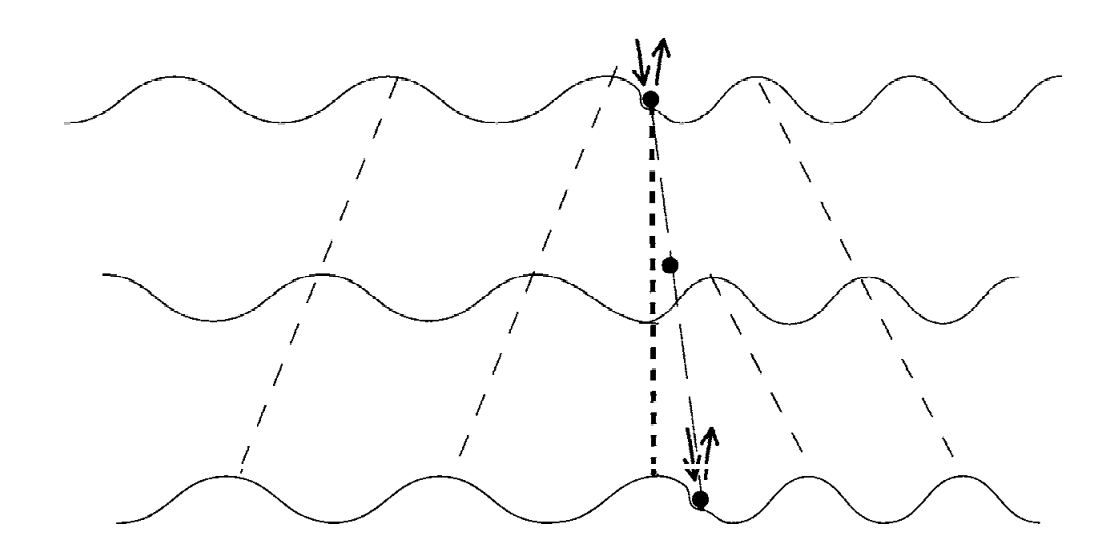
\includegraphics[width=12cm]{theory/walkingDroplet}
\centering
\caption{An illustration of a walking droplet's motion for subsequent bounces. The movement of droplet is exaggerated for visual purposes. In reality, wave amplitude decays with distance from droplet and is not necessarily constant; it is modulated by the driving force. }
\centering
\label{walker}

\end{figure}

Equations of motion for this droplet motion described above were taken from \cite{oza2013trajectory}, which showed that the surface wave produced on the $\textrm{n}^{\textrm{th}}$ impact of a particle at position $r_n$ and time $T_n$ on a surface oscillating vertically at $\omega$ above the Faraday threshold is given by (\ref{equ:heightSurfaceWave}). Here, $ h(\vec{r} , t)$ is the height of the wave at $\vec{r}$, $J_0$ is a Bessel function of the first kind, and wave number $k$ satisfies the relation $ J_0 \left( k \vec{r_0} \right) = 0$. $\vec{r_0}$ is a numerical cutoff parameter, while the amplitude of the wave, A is material specific and determined by the system parameters used. The exponential decay term at the end of the equation describes the wave decaying over time at a rate determined by the memory $Me$ and period of particle $T_f$.

\begin{equation}
h_n(\vec{r} , t) = A J_o\left(k\left|\vec{r} - \vec{r_n}\right| \right) e^{-\frac{\left(t-T_n\right)}{T_f Me}}
\label{equ:heightSurfaceWave}
\end{equation}

The overall surface wave can thus be described by the sum of all waves produced by every prior impact. Assuming the particle only interacts with the surface once every period (when the particle is at its lowest point), the overall wave equation $h (\vec{x} , t)$ is thus given by (\ref{equ:heightSumSurfaceWaves}).

\begin{equation}
h(\vec{r} , t) = \sum_{n=-\infty}^{\frac{t}{T_f}} A J_o\left(k\left|\vec{r} - \vec{r_n}\right| \right) e^{-\frac{\left(t-n T_f\right)}{T_f\times Me}}
\label{equ:heightSumSurfaceWaves}
\end{equation}

Furthermore, we know that the surface wave needs to consider relativistic effects. The coordinate transform on the wave formed by the $n^{\textrm{th}}$ impact of a particle at some velocity v is as follows:
\begin{equation}
h_n(\vec{r} , t) = A_0 cos\left(\omega_0 t - \frac{\gamma^2 \omega_0 v}{c^2}\right) J_0\left(k \left| \left(\vec{r} - \vec{r_n}\right)^{\prime \prime}  \right| \right)e^{-\frac{\left(t-n T_f\right)}{T_f\times Me}}
\end{equation}

Where:
\begin{equation}
\gamma = \frac{1}{\sqrt{1-\frac{v^2}{c^2}}}
\end{equation}
\begin{equation}
\left(\vec{r} - \vec{r_n}\right)^{\prime \prime} = \gamma^2(\vec{r_v}-\vec{v}t)+\gamma\vec{r_{\perp}}
\end{equation}

$\vec{r_v}$ and $\vec{r_{\perp}}$ are the components of $\left(\vec{r} - \vec{r_n}\right)$ in the direction of velocity and perpendicular to velocity respectively.

\subsection{The memory parameter $Me$}
The memory parameter,  $Me$ , represents the decay time of a wave produced from a given impact in terms of the time between each impact. It is defined by the ratio between the non-dimensional damping time $\tau$, and the Faraday period of the system $T_f$.
A droplet entering a walking state is a direct result of this memory parameter and can seen by the comparison of the high and low memory regimes \cite{couder11}.
In the high memory regime, the waves decay slowly, and so waves created in the distant past can still strongly influence the particle trajectory. However, in the low memory regime, the waves decay rapidly, so only waves created in the recent past can significantly influence the particle's trajectory. 


\todo{Subsection on multiple droplet interaction}
\subsection{May need section on interaction between multiple droplets if we use that data}
\todo{Fluid dynamics stuff}
\subsection{Fluid Dynamics}
If the height of the oil is known for the entire surface, the trajectory after a bounce at any point can be calculated using basic equations of motion. On collision, the impulse received by the droplet is found to be proportional to the gradient of the surface. This can then be used to find the velocity until the next collision. 
\clearpage

\section{Experimental Method (SV, KF, BB)}

This section fully explains the processes undertaken in order to complete this project. It includes  information regarding personnel involved, expenditures undertaken and relevant venues, as well as a full, detailed list of equipment used.

\subsection{Equipment list}

In its final iteration the experimental apparatus...\todo{Apparatus description}

Below is a full list of equipment used in various stages of the experiment. More information about how each piece of equipment is utilised is included in the following sections.
\bigskip
\begin{enumerate}

\item \textbf{Speaker: QXW6 6.5'' High Power Woofer with Kevlar Cone - QTX \ref{fig:speaker}:}

\begin{itemize}
\item 250W power max
\item 8$\Omega$ impedance
\item 1.92kg
\item 88.0dB
\item Frequency Response: 35Hz - 8kHz
\item Overall depth: 90mm; Diameter: 16.5cm
\end{itemize}
\item \textbf{Liquids:}

\begin{itemize}
\item 1000 cSt silicone Oil - From Derreck
\item 50 cSt silicone Oil - Alfa Aesar, 63148-62-9, L05379
\item Fairy Liquid washing up liquid
\item Water
\item Sunflower oil - Sainsbury's
\end{itemize}
\item \textbf{Recording Equipment:}

\begin{itemize}
\item Photron Fastcam SA1.1 Type 675K M1 \ref{fig:PhotronCamera}

\begin{itemize}
\item Input DC20-36V / 130VA
\item Resolution of 1024 x 1024 pixels at 5400fps
\item Maximum framerate of 675,000fps at resolution of 64 x 16
\end{itemize}
\item Lumix flash camera with GVaro 14-42 zoom lens 1:3.5 - From Kelvin Vine (Physics Film Makers)
\item Photron Spectrum Lumination P/N EL2150-WHI lighting \ref{fig:PhotronLighting}

\begin{itemize}
\item Manfrotto Photo Variable Friction Arm with Bracket, SKU 244
\end{itemize}
\item iPhone X, iOS:11.1.5 , published recorded rate: 240 fps

\item Sony Cyber-shot RX-100 IV Camera, 4K, 20.1MP, 2.9x Optical Zoom, Wi-Fi, NFC, OLED EVF, 3'' Tiltable Screen (1000fps camera)
\item Diffuser
\item High powered lighting - TriLite Max 3x30W Compact Flourescent Lamps 220-240V. Bowens, 3.15A (F)
\end{itemize}
\item \textbf{Software:}

\begin{itemize}
\item Photron FASTCAM Software - PFV Ver.3681
\item Adobe AfterEffects CS6
\item Adobe Premiere Pro CS6
\item Adobe Illustrator CS6
\item Google Sketchup
\item Sound Meter - Mobile App
\end{itemize}
\item \textbf{Machinery - Institute of Making:}

\begin{itemize}
\item Lasercutter
\item Bandsaw
\end{itemize}

\item \textbf{Signal Generators / Amplifier:}

\begin{itemize}
\item Griffin signal generator and amplifier \ref{fig:griffinsSigGen}
\item ISO-TECH Synthesized function generator GFG2004 
\item Hi-Fi amplifier ELEGIANT mini 20W 12V hi-fi car stereo amplifier LP-838 \ref{fig:amplifier}

\begin{itemize}
\item Kasstino Power Supply Adapter 12V AC 100-240V To DC 12V 2A 24W for LED Strips
\end{itemize}
\end{itemize}
\item \textbf{Miscellaneo:}

\begin{itemize}
\item Cardboard square
\item Circular plywood plate
\item 3.5'' glass petri dish - from Chemistry (2nd Floor Turner Labs, Christopher Ingold) \ref{fig:PetriDish}
\item 6'' plastic petri dish - from Chemistry (2nd Floor Turner Labs, Christopher Ingold)
\item Square tupperware box (135mm x 135mm)
\item LE LED USB Light Strip, SKU: 4100072-RGB

\begin{itemize}
\item Power: 5W
\item 16 lighting colours
\end{itemize}
\item Optical microscope
\item Soldering iron \& solder
\item Plastic strips - from plastic binder
\item Plastic pipette (1mm \& 3mm) - from Chemistry (2nd Floor Turner Labs, Christopher Ingold) chemistry lab
\item Digital Thermometer - 2000T - \ Thermometer, -200$\degree$C to +1350$\degree$C, 155 mm, 67 mm, 40 mm Type Input, Intrinsically Safe
\item Multimeter
\item 3mm Laser grade plywood
\item Red food colouring

\begin{itemize}
\item ASDA natural food colouring - red
\item Dr Oetker bright red gel food colour 15g
\end{itemize}
\item Electric cables

\begin{itemize}
\item BNC cables
\item Banana plugs (amplifier to speaker)
\item 3.5mm jack to aux (laptop to amplifier)
\end{itemize}

\item Double sided tape
\item Plastic \& glass syringe - from Andrew Redfearn
\item Spray duster - Dataflash, DF1270
\item Knitting Needle \ref{fig:DropletCreators}
\item Wood cuttings

\begin{itemize}
\item Grated cuttings - leftover from laser cutting \ref{fig:DropletCreators}
\item Solid blocks - from IoM
\end{itemize}
\item Foldback clips (clamps) - Q-Connect, 42mm
\item 1mm graph paper - Chartwell, A4-641C
\item Superglue - UHU
\item Metal ruler - 30cm
\end{itemize}
\end{enumerate}

\begin{figure}[ht]
    \begin{subfigure}{0.5\textwidth}
        \centering
        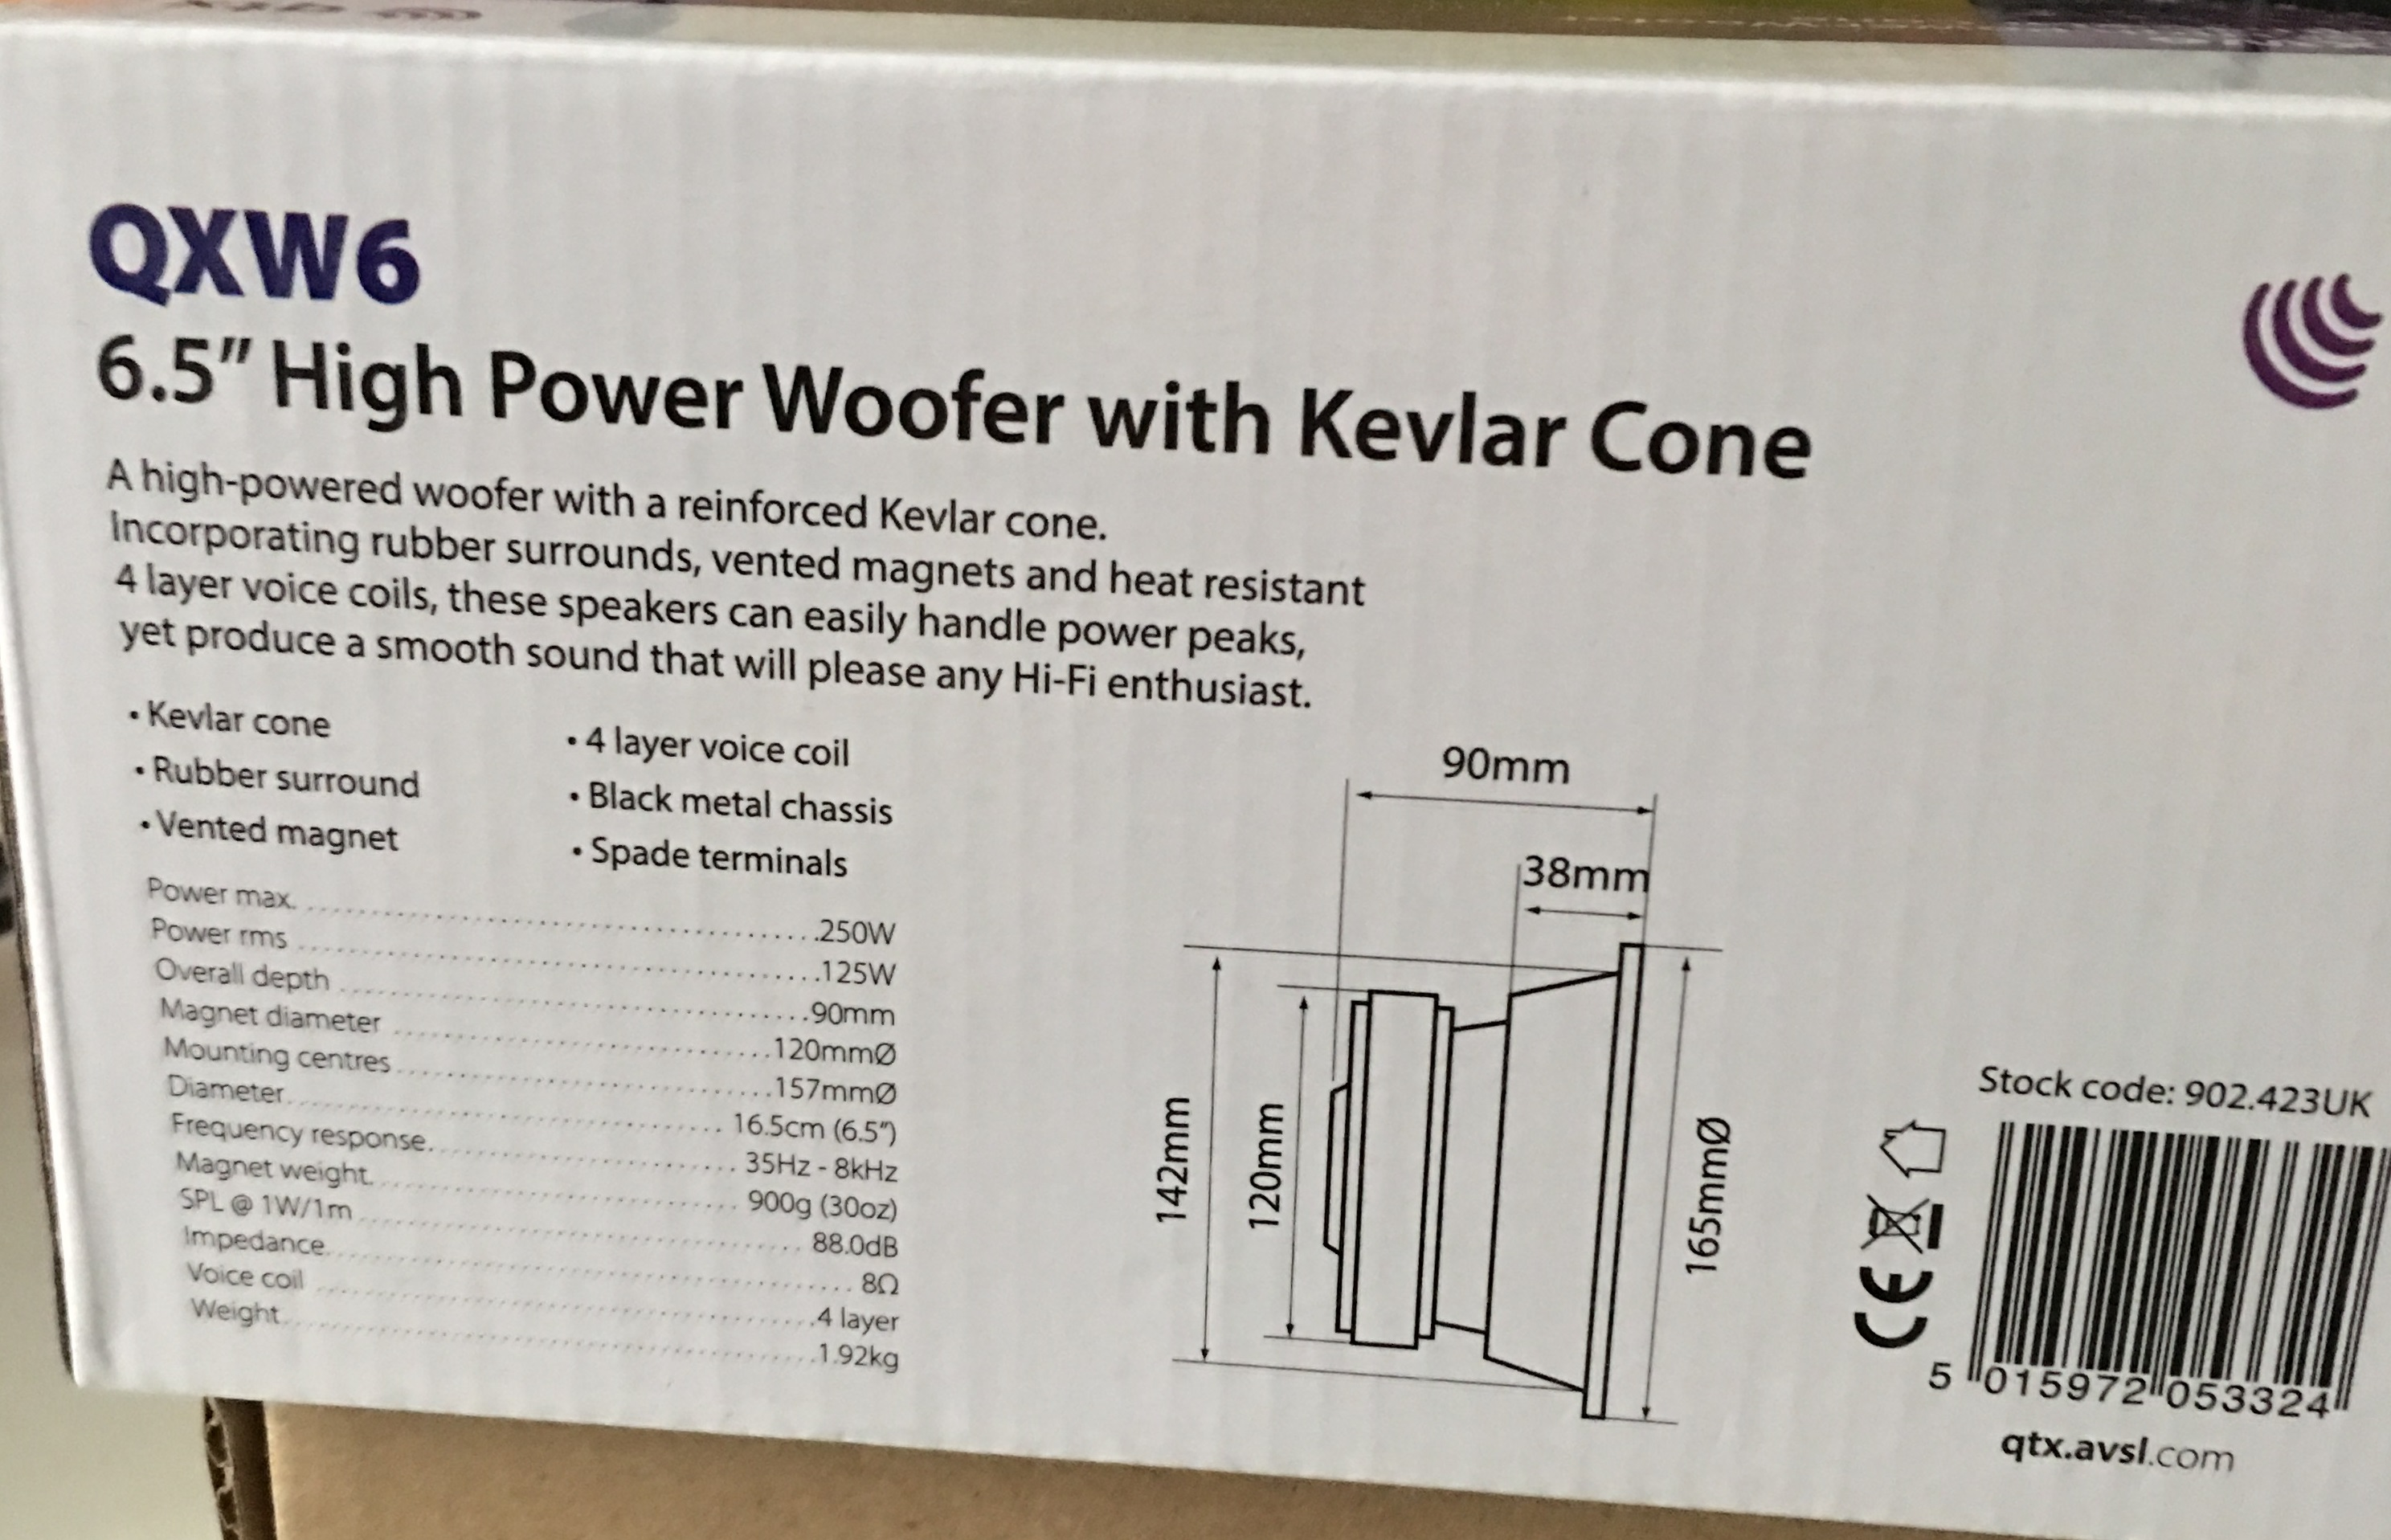
\includegraphics[width=\textwidth]{prototype/exp_rep_imgs/speakerPackaging.jpg}
        \caption{Packaging of the woofer used}
    \end{subfigure}
    \begin{subfigure}{0.5\textwidth}
        \centering
        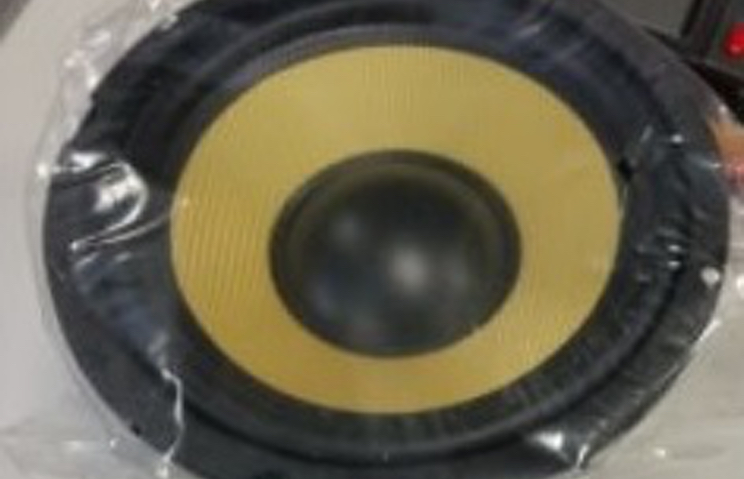
\includegraphics[width=\textwidth]{prototype/exp_rep_imgs/Speaker.jpg}
        \caption{The woofer used to carry out oscillations}
    \end{subfigure}
\caption{Images of the speaker and its packaging utilised in vibrating the liquid surface. The packaging image provides technical information regarding the woofer and its dimensions}
\label{fig:speaker}
\end{figure}

\begin{figure}[ht]
    \begin{subfigure}{0.5\textwidth}
        \centering
        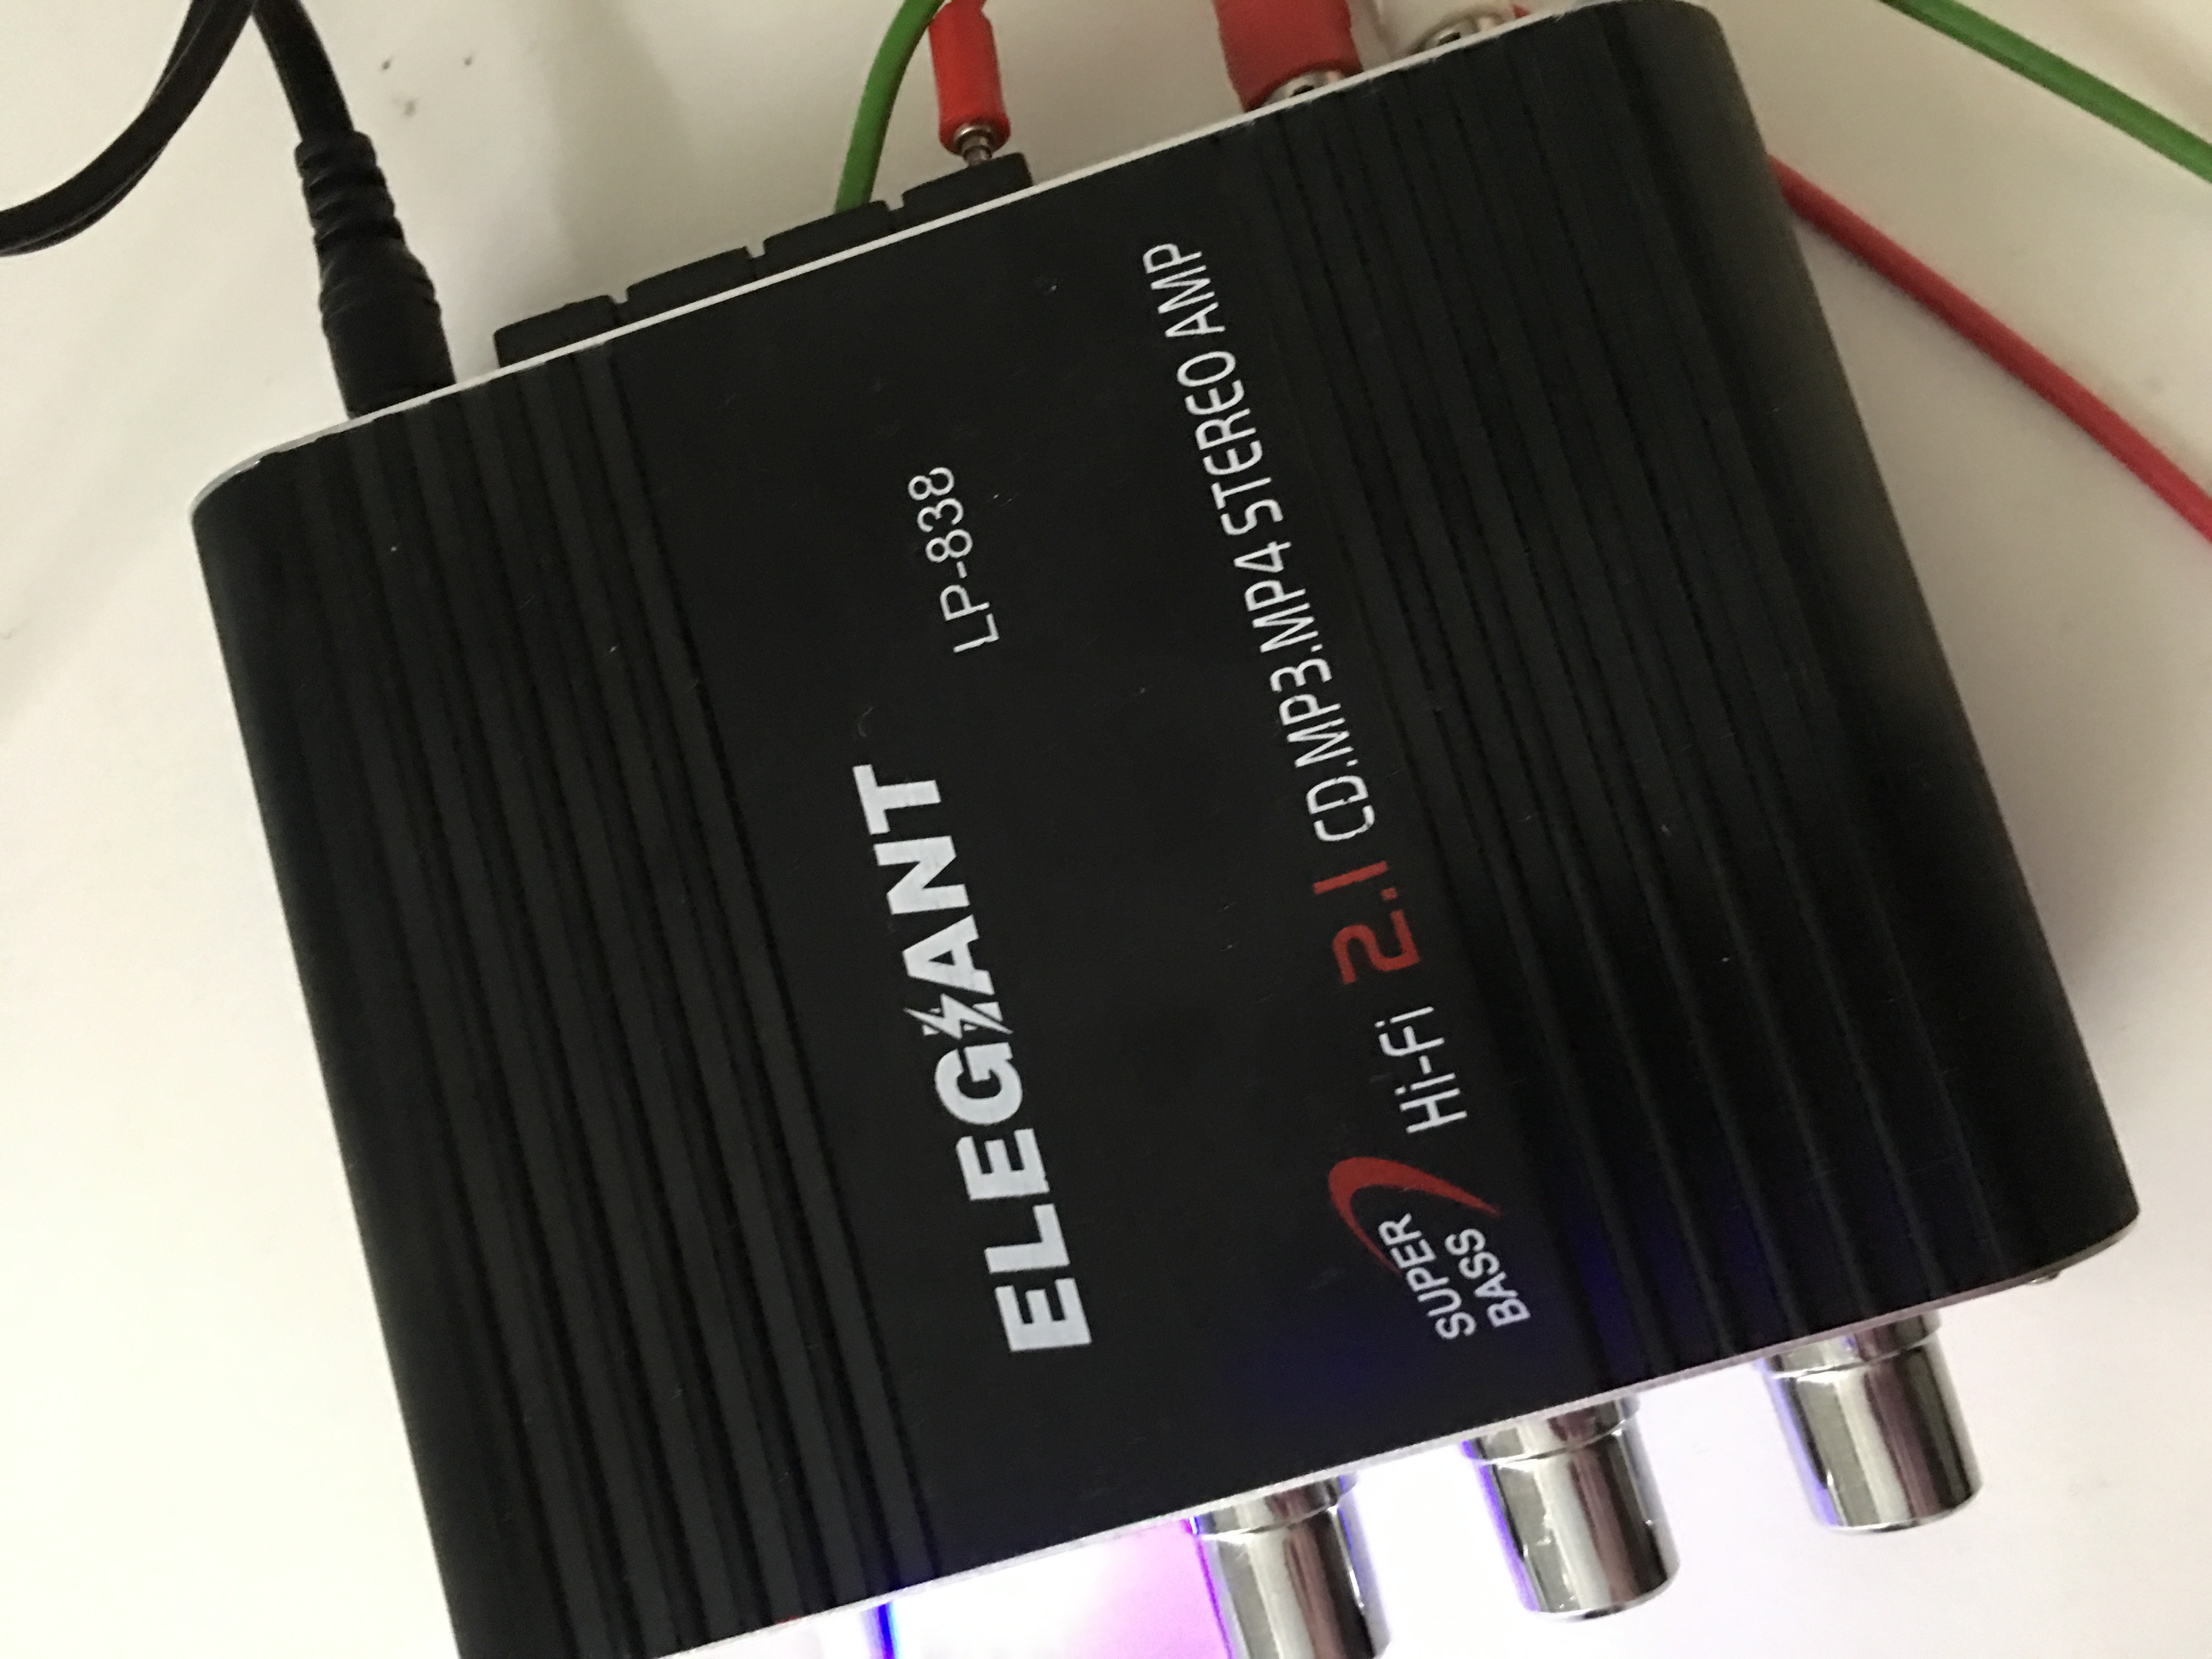
\includegraphics[width=\textwidth]{prototype/exp_rep_imgs/LEGIANT_amp.jpg}
        \caption{Top-down image of the amplifier}
    \end{subfigure}
    \begin{subfigure}{0.5\textwidth}
        \centering
        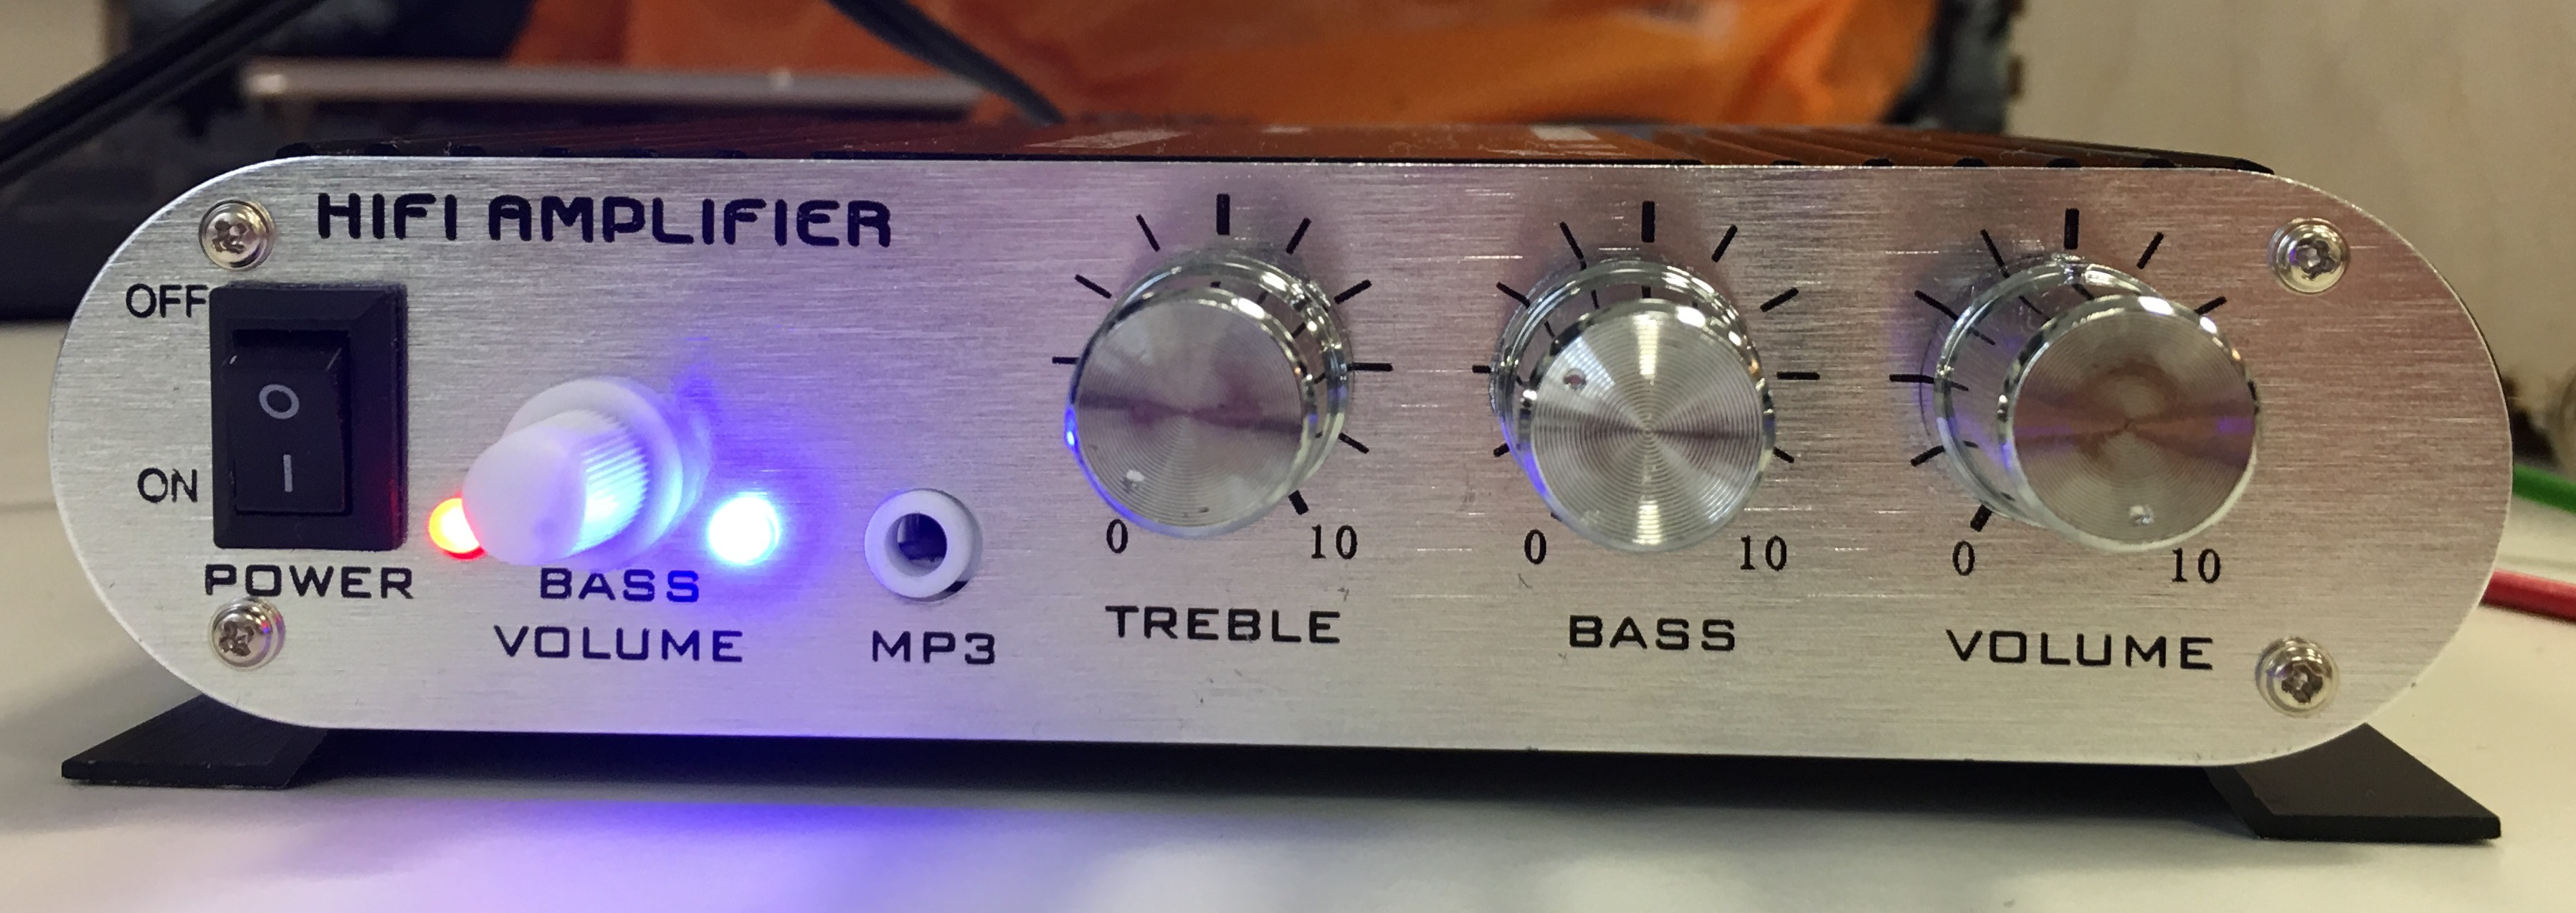
\includegraphics[width=\textwidth]{prototype/exp_rep_imgs/amp_controls.jpg}
        \caption{Image detailing the layout and variety of controls available to us with the amplifier.}
    \end{subfigure}
\caption{Images of the ELEGIANT Mini 20W 12V Hi-Fi Car Stereo Amplifier used to boost the input from the signal generator, in order to allow for vibrations of sufficient magnitude to produce droplet motion.}
\label{fig:amplifier}
\end{figure}

\begin{figure}[ht]
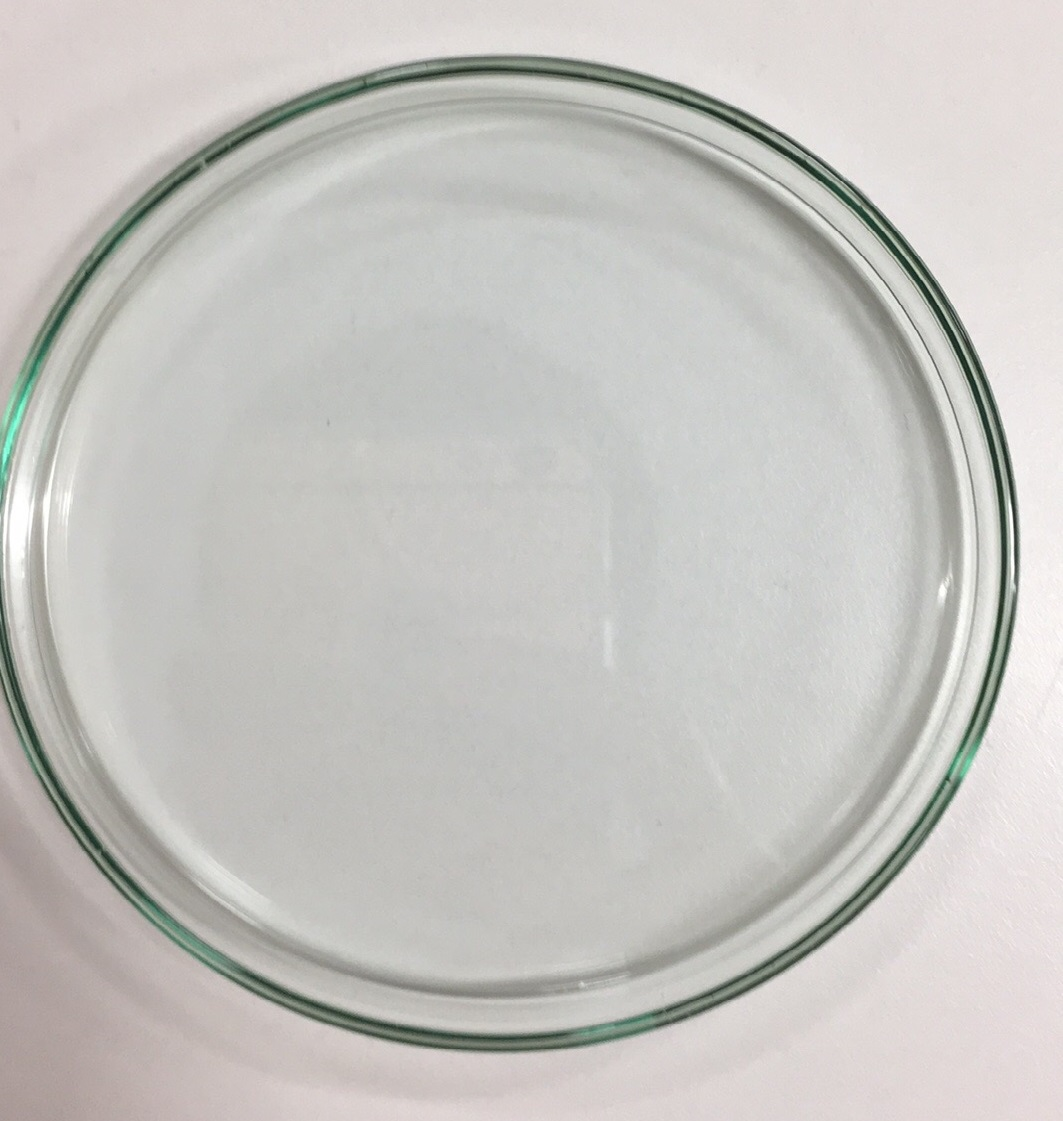
\includegraphics[width=12cm]{prototype/exp_rep_imgs/petriDish.jpg}
\centering
\caption{An image of the 4" petri dish used to house the liquid used as a surface in this experiment.}
\centering
\label{fig:PetriDish}
\end{figure}

\begin{figure}[ht]
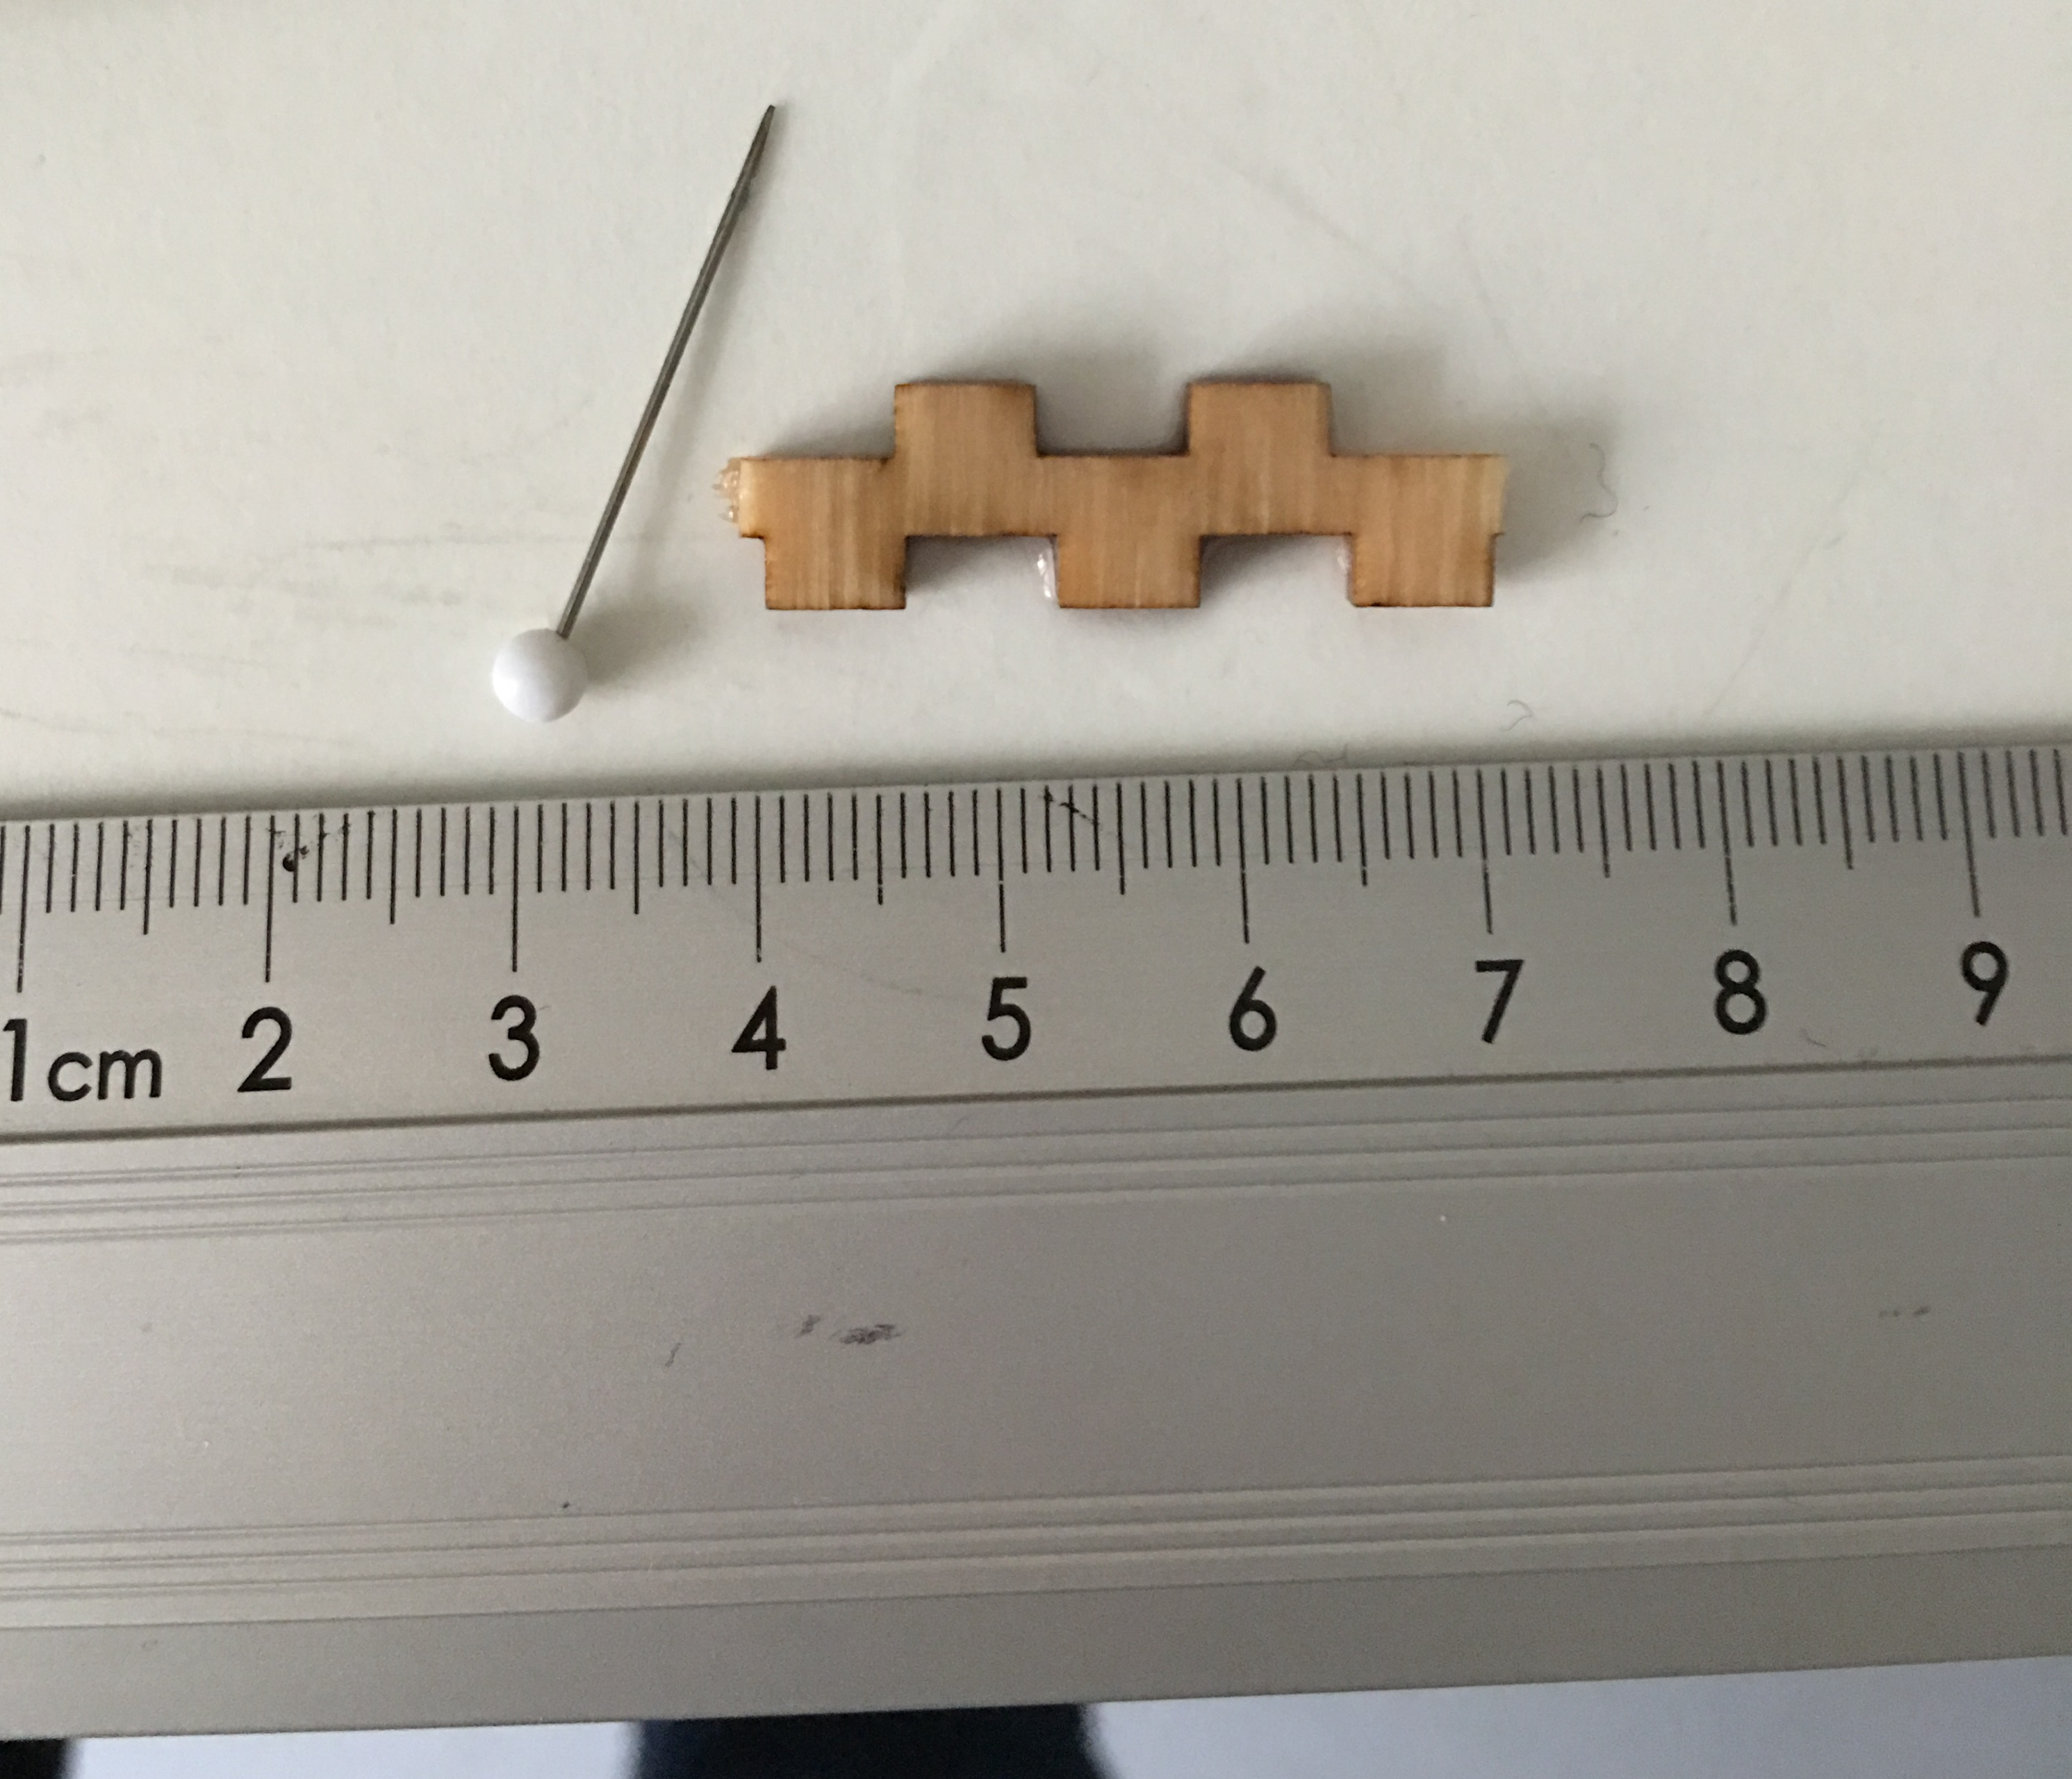
\includegraphics[width=12cm]{prototype/exp_rep_imgs/DropletCreators.jpg}
\centering
\caption{An image of a needle and glued together plywood remnant of the laser-cutting process, used to generate droplets for experimentation.  The plywood remnant was well suited to producing multiple droplets consistently, but using the needle to produce droplets proved to be difficult. It was instead utilised to destroy unwanted droplets. A ruler is placed alongside for scale  }
\centering
\label{fig:DropletCreators}
\end{figure}

\begin{figure}[ht]
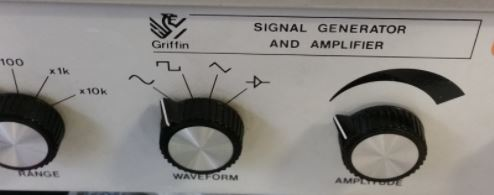
\includegraphics[width=12cm]{prototype/exp_rep_imgs/griffinsSigGen.jpg}
\centering
\caption{An image of the Griffins Signal generator initially used in this experiment. It had a in-built amplifier that helped boost the signal.}
\centering
\label{fig:griffinsSigGen}
\end{figure}

\begin{figure}[ht]
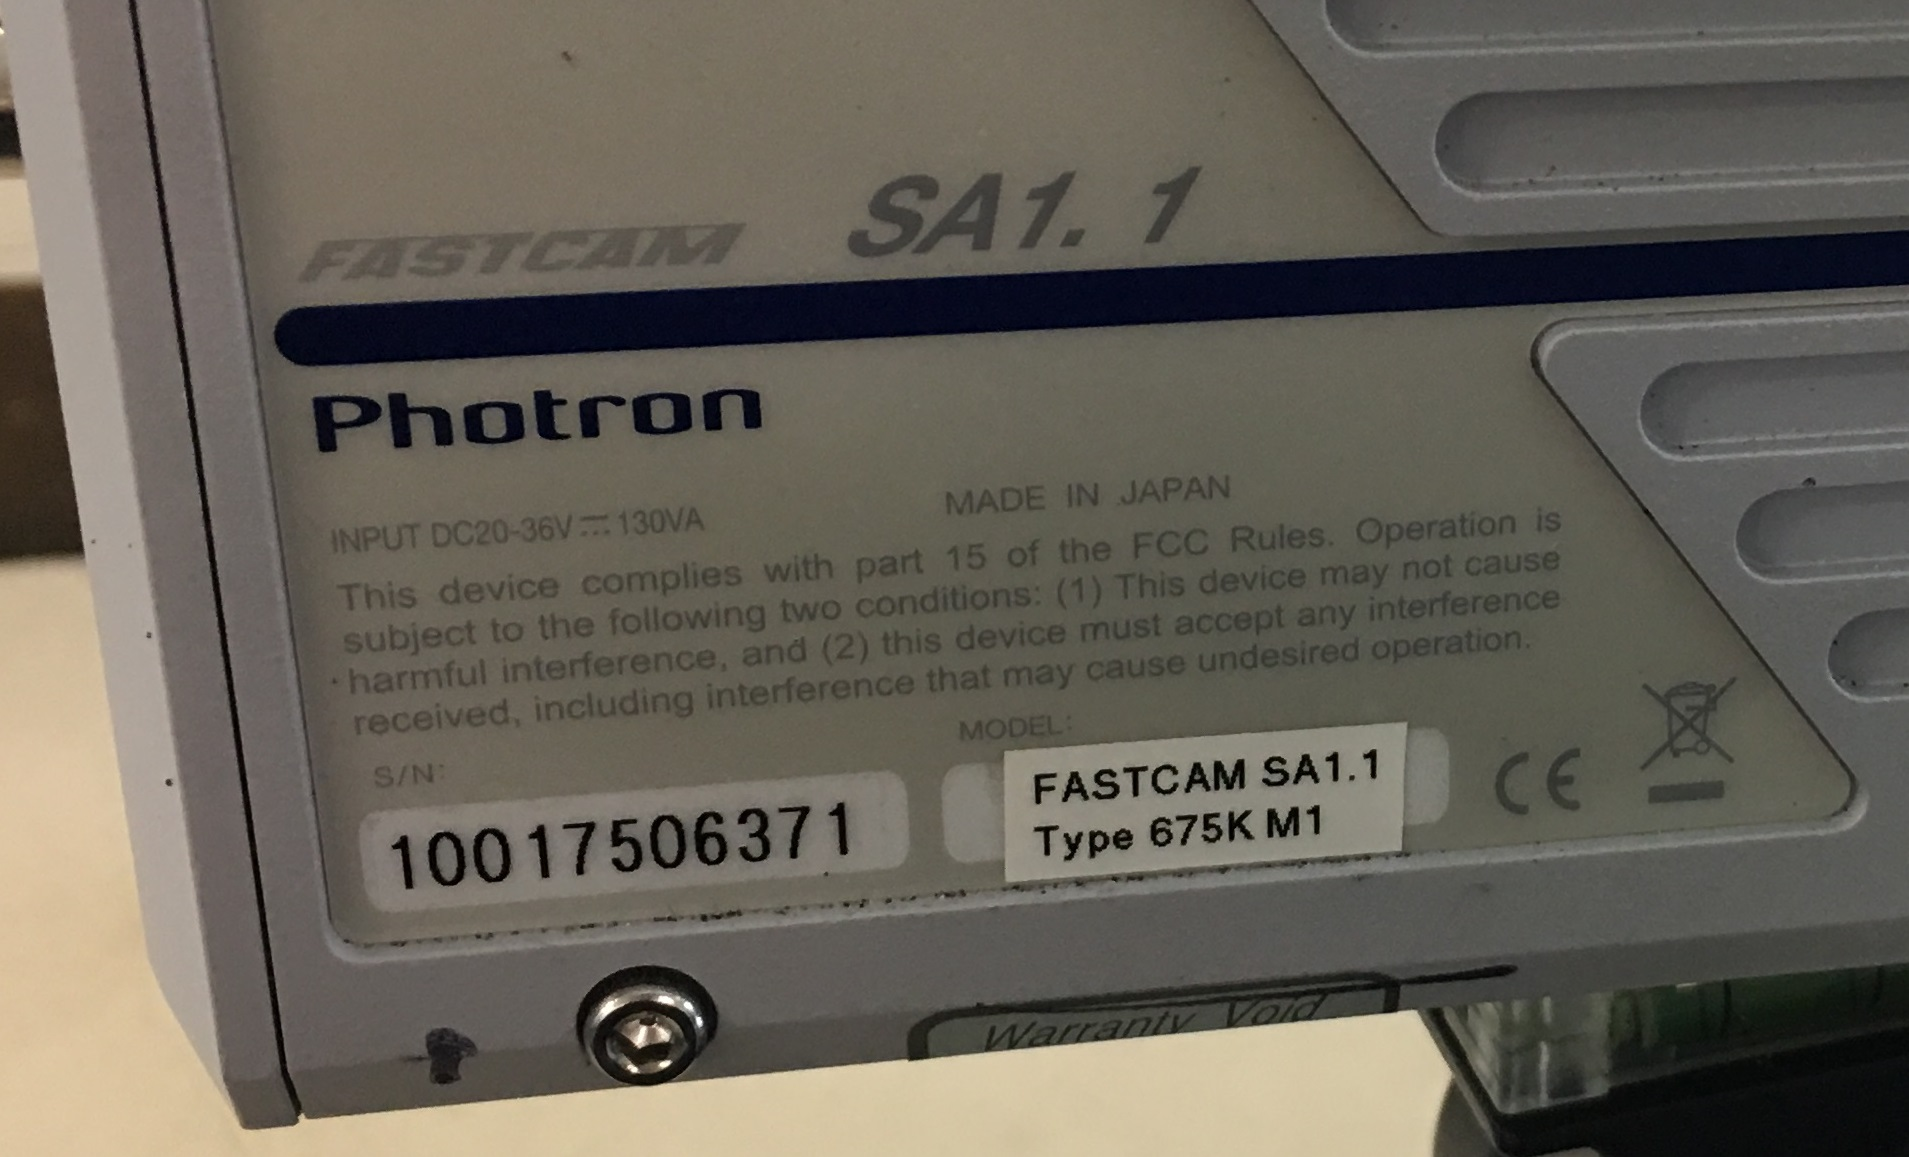
\includegraphics[width=12cm]{prototype/exp_rep_imgs/PhotronHighSpeedCamera.jpg}
\centering
\caption{Side view of the Photron Fastcam SA1.1 Type 675K M1 high speed camera used to capture the droplet motion at 1000 fps. The camera was controlled via a laptop installed with PFV Ver.3681, where settings such as resolution and frame rate could be modified.}
\centering
\label{fig:PhotronCamera}
\end{figure}

\begin{figure}[ht]
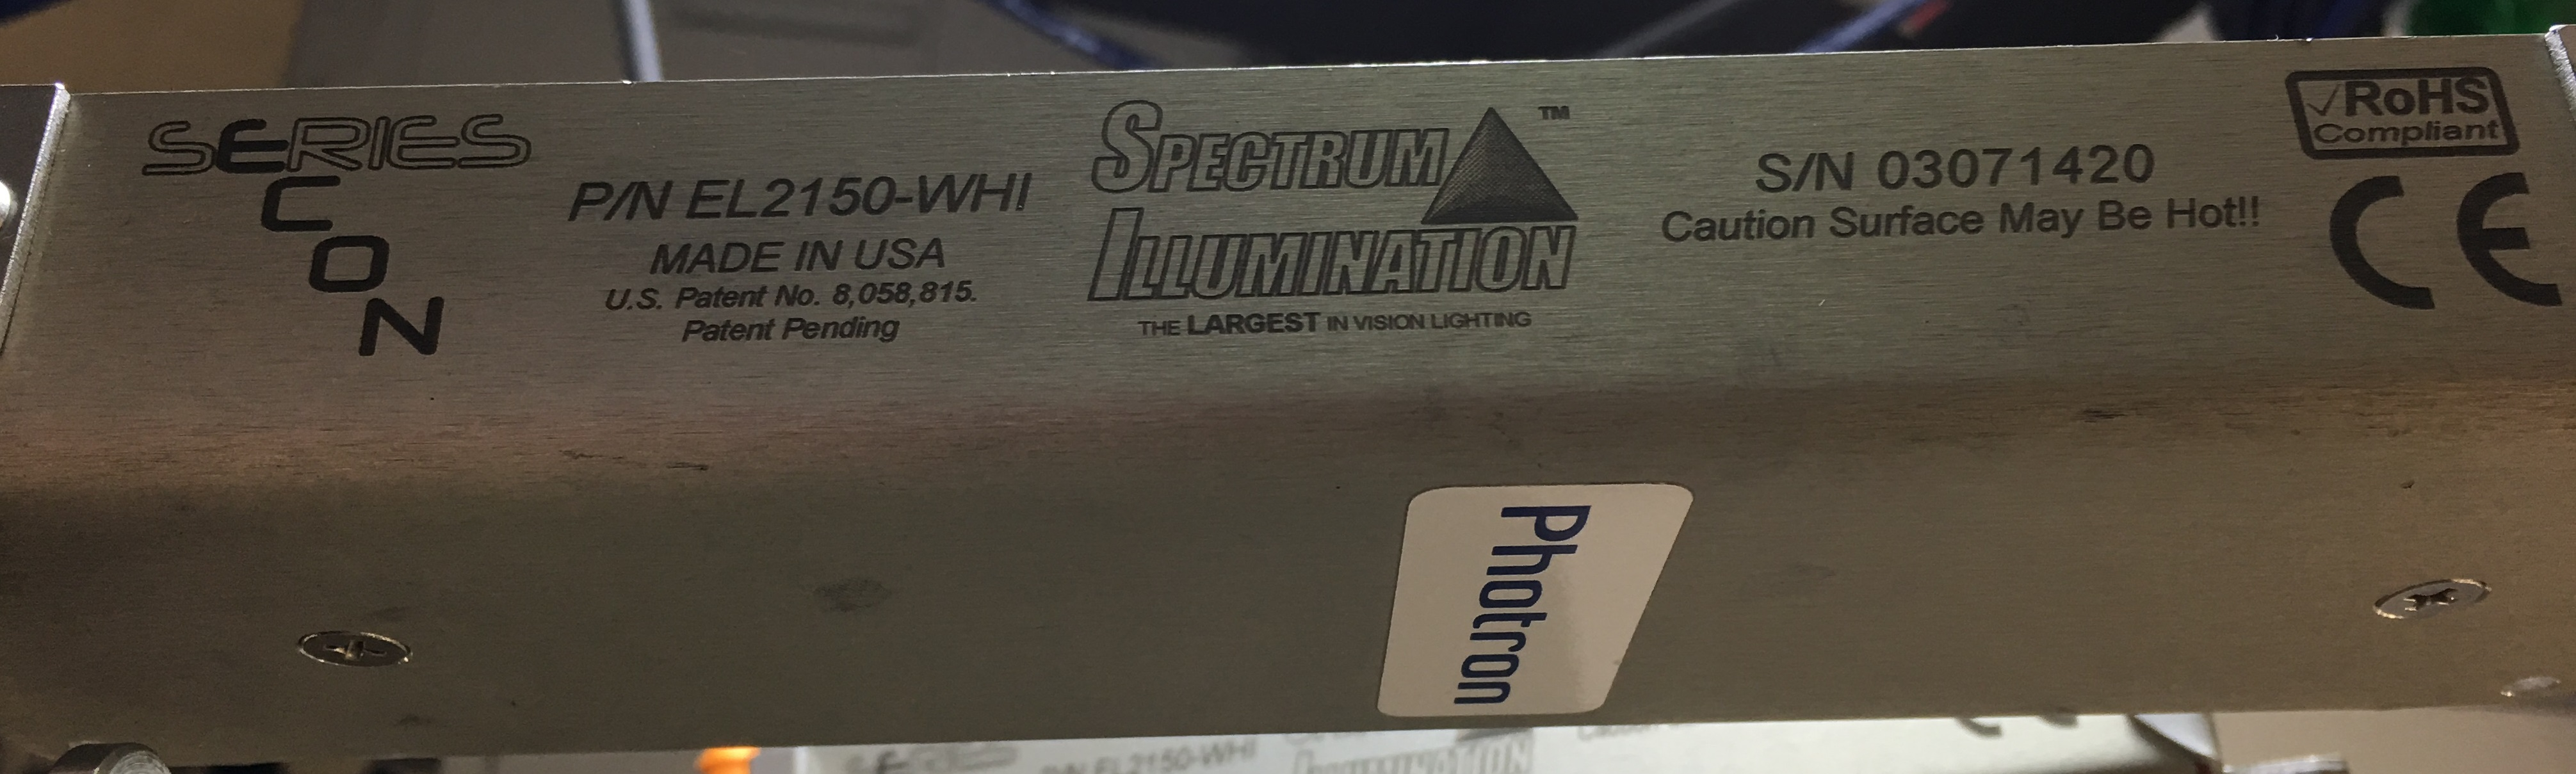
\includegraphics[width=12cm]{prototype/exp_rep_imgs/PhotronLighting.jpg}
\centering
\caption{Photron Spectrum Lumination P/N EL2150-WHI lighting uused to illuminate the droplets for high speed recording. The use of powerful lights is necessary to ensure clear recordings/images for high speed recording, due to the high shutter time and low light exposure.}
\centering
\label{fig:PhotronLighting}
\end{figure}

\subsection{Sourcing of Equipment}

To construct a preliminary experimental setup, the topic was investigated by an online search, and subsequent review of peer-reviewed papers. A list of equipment was compiled, with prices and links for purchase. This was partnered with alternative options as backups, in case of time concerns, budgeting issues or extensions to the experiment. Due to the limited budget of \pounds200, it was decided that the team would try to source as much of the equipment as possible for free. This was particularly vital, considering the preliminary fixed cost of \pounds40 that had to be set aside for poster printing.

The following steps were taken by our team in self-sourcing of equipment. This was to gain knowledge on certain equipment, borrowing them or seeking further assistance.

\begin{enumerate}
\item  Contact was made with the Mechanical Engineering department on the 5th floor of  Roberts building. We were able to order an `off the shelf' amplifier.  They were also able to provide us with a 3.5 mm jack to aux cable.
\item  Contact was made with Mychal Riley from Mechanical Engineering to enquire about borrowing a high speed camera. He provided us with a contact - Dr. Han Wu from 224  Chemical Engineering, who was in possession of a suitable device.
\item  After further exploration of the offices on the 4th floor of Roberts  building, a person referred us to Andrew Redfearn, who had equipment for professional video capturing.
\item  Contact was made with the owner of a camera shop near Tottenham Court Road station  - Parl Cameras: Rathbone Pl, Fitzrovia, London W1T 1JR
\item  A petri dish (4") was borrowed from the Chemistry department, from the Turner Lab  on the 2nd floor of Christopher Ingold building.
\end{enumerate}

The central piece of equipment was the loudspeaker. The main considerations were the power, dimensions and functions. It was decided that online purchases should be carried out with Amazon Prime due to its next day delivery service. The speaker was a 902.423UK 20W Woofer manufactured by QTX. The packaging and the actual device itself are displayed in Figure \ref{fig:speaker}.

Structural integrity and the ease of replicability were our primary considerations when designing the housing for the speaker and petri mount. After consulting staff at the Institute of Making (IoM), it was decided that laser cutting a template out of laser grade plywood would fulfil our base requirements. By using the free laser cutting case designer wasp provided by MakerCase (\url{http://www.makercase.com}), a template for the housing was generated. This allowed the housing to be replicable provided that access to a laser cutter and laser grade plywood was available. By incorporating finger joints in the design, the housing was sturdy enough to retain structural integrity when driving the speaker at maximum power output within the frequency range used without any adhesive or screws. The blueprint for the template is shown in Figure \ref{fig:blueprint}. It was designed to match laser grade plywood of 3 mm thickness.

\begin{figure}[htbp]
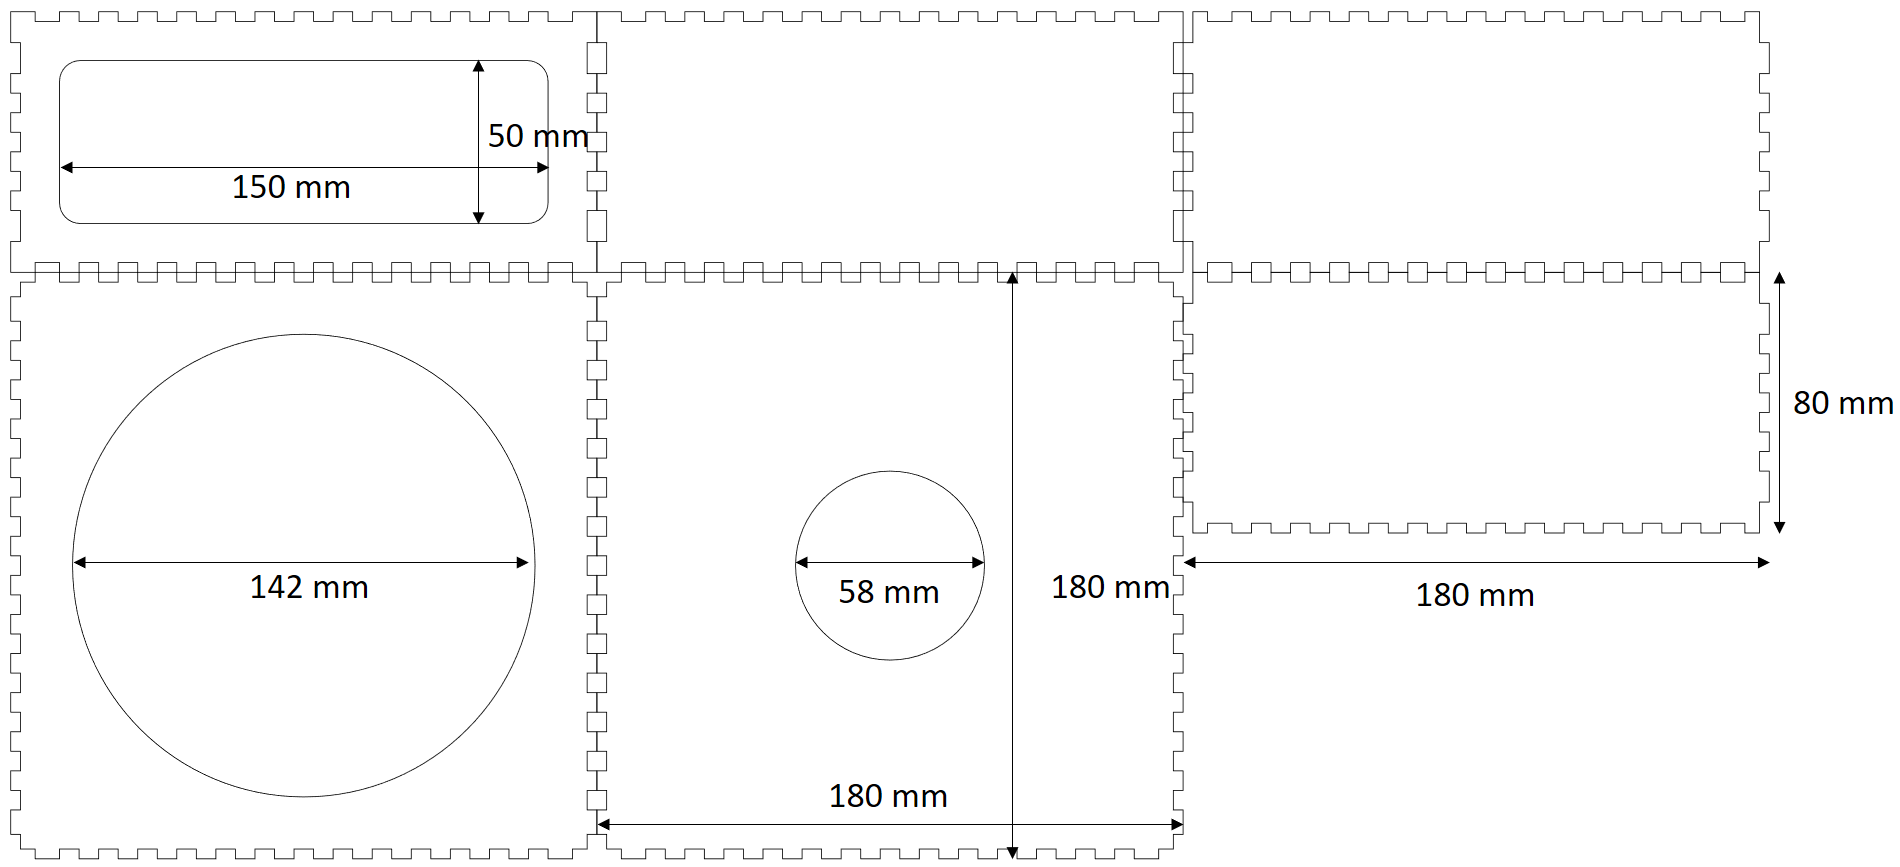
\includegraphics[width=\textwidth]{prototype/exp_rep_imgs/Blueprint.png}
\centering
\caption{Blueprint used in laser cutting the box that was used to house the loudspeaker. The blueprint provides the exact dimensions for the different components of the box before they were attached together.  }
\centering
\label{fig:blueprint}
\end{figure}

Measurement errors in the template resulted in the housing being 6mm too short for the speaker, causing the base of the speaker to protrude slightly out of the housing, thus making the housing unevenly balanced. To account for the height issue, two 3mm pieces of plywood were glued together and cut into 4 narrow strips. The strips were then glued to the housing to act as supporting platforms to hold up the speaker. To correct for the protruding speaker base, an additional copy of the bottom face of the housing was cut and glued onto the base of the housing. This ensured that the housing was properly levelled.

Were we afforded more time, we would ideally use a stronger material to  re-print the housing, possibly with stabilisers or a damping material, so that vibrations are driven directly into the fluid more efficiently rather than the box or surrounding platform. This perhaps could have been achieved by layering the base of the speaker with sand to damp unwanted vibrations.

The next step involves placing the speaker into the box. This process can be seen in Figure \ref{fig:boxassembly}.

\begin{figure}[ht]
\centering
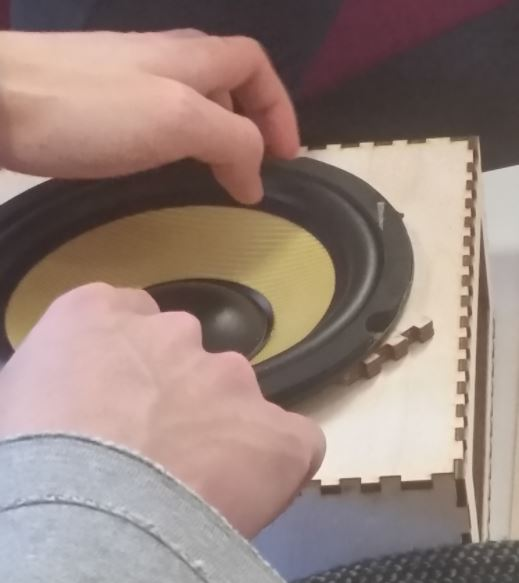
\includegraphics[width=0.5\textwidth]{prototype/exp_rep_imgs/boxAssembly.jpg}
\caption{A snapshot of the loudspeaker mounting process undertaken as part of the initial assembly stage. One of the cut pieces of plywood used to support the speaker is also visible here.}
\label{fig:boxassembly}
\end{figure}


\subsection{Testing of Loudspeaker}
Preliminary testing was conducted using an ISO-TECH synchronized function generator GFG2004. A detectable signal was picked up by the loudspeaker, where the diaphragm was clearly vibrating and producing sound. However, the signal was found to be too weak to cause vibrations in a petri dish. The team then tried to source a function generator that offered a higher output power. The Physics Laboratory was able to provide a Griffin function generator that allowed for amplification. It was decided that the team would have to attempt produce droplets with this function generator before purchasing an amplifier.

\subsection{Experimentation with 1000 cSt silicone oil}
A full experimental run  was carried out by connecting the Griffin function generator to the loudspeaker, in order to drive a petri dish of 1000 cSt silicone oil. Double sided tape was used to stick a square cardboard plate onto the loudspeaker's edge/diaphragm intersection and then sticking the petri dish onto the cardboard. This was to avoid damaging the diaphragm. However a concern was raised regarding the ability of the cardboard plate to fully transmit the vibration of the loudspeaker. Sticking the petri dish onto the diaphragm with adhesive was considered as a final resort.

About 4 mm of silicone oil was poured into the 4'' petri dish. This was measured using a metal ruler that was aligned to the base of the petri dish. A frequency range of 50 -- 100 Hz was tested, adjusted via the frequency generator.

Using a needle to quickly flick the surface of the oil, unsuccessful attempts were made to produce droplets. This was thought to be due to the high viscosity of the oil, as droplets were observed to stay on the tip of the needle even after rigorous attempts to dislodge them. In the rare occasions where droplets were actually produced, they did not last for long before coalescing with the liquid. The droplet diameter was also very large ($>$1mm) and the droplets appeared to be sitting on the surface instead of bouncing. Different methods were tried, including releasing droplets from a low height. However there was little chance to observe actual bouncing, or to produce sustainable droplets in order to test other phenomena.

As a result,  many possible improvements were considered. It was not clear what the major problem was, but it  could have been caused by the low driving amplitude, which did not provide enough acceleration to allow for bouncing. The other was the high viscosity of silicone oil. It was also decided that the square cardboard plate had to be replaced due to its lack of rigidity. Air was observed to escape from the side of the loudspeaker, which meant that energy was lost and not transmitted to the petri dish. 

It was decided that improvements were to be carried out immediately, hence the decision to purchase an ELEGIANT qroiip2097 20W amplifier. This was accompanied by a Sunydeal 60W power cable.

The cardboard plate was replaced with a circular 3 mm thick plywood cut-out, a by-product of the laser-cutting process. It was found that the diameter was slightly too small, as it was not able to reach the outer edge of the loudspeaker. Despite this, the new plywood plate was still large enough to be secured with double-sided tape. 

A lower viscosity silicone oil (50 cSt) was obtained from the Turner Lab in the Chemistry Department. These improvements were subsequently incorporated into the equipment.

\subsection{Experimentation with 50 cSt silicone oil}
With the lower viscosity silicone oil and the improved setup, a second attempt was made to produce droplets. The amplifier knobs allowed the adjustment of treble, bass and volume. The amplifier input was connected to the function generator's output via a 3.5 mm jack to aux cable and a pair of banana plugs. The output was connected to the loudspeaker's input with banana plugs. This setup can be seen in Figure \ref{fig:exp_setup_sideshot}.

\begin{figure}[ht]
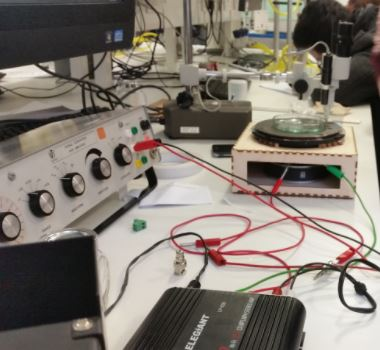
\includegraphics[width=0.5\textwidth]{prototype/exp_rep_imgs/exp_setup_sideshot.jpg}
\centering
\caption{The experimental setup in testing the 50 cSt silicone oil. This setup used an amplifier connected to the Griffin function generator, and the amplifier output was connected to the loudspeaker via crocodile clips.  }
\centering
\label{fig:exp_setup_sideshot}
\end{figure}

To maximise the transmitted signal, the function generator was set to minimum attenuation and connected via the 4 ohms impedance output to match the impedance of the speaker. A smart phone was also tested. The results were very similar to that of the function generator, but the phone provides an advantage in terms of accessibility and ease of use.

The output wave was tested in a frequency range of 50 -- 80 Hz. Bouncing droplets that persisted for minutes were produced. High volume and bass were found to be beneficial for producing high-bouncing droplets. It was discovered that the frequency range corresponded to bass, thus both knobs work similarly.

Some droplets also appeared to 'walk'. However it was uncertain if they were indeed exhibiting a 'walking' phenomenon or was it due to an external force. This is because any form of breeze in the laboratory could easily move the droplets; talking could also have produced enough pressure to move them. It was also possible to combine droplets together, forming crystal lattice-like structures.

Using the slow-motion video capturing mode on iPhone, the droplet behaviour and motion were captured. It was found that the droplet size was too small to be accurately determined by the naked eye or with a photograph. An alternate method was proposed: viewing the droplet through a microscope borrowed from Physics Lab 3. However after several attempts to focus the lens and lighting, it was found to be non-feasible, and the idea was not investigated further.

Improvements were proposed to improve the setup. It was decided that graph paper could be taped underneath the petri dish. The grid would provide a useful way to track the droplet's motion and size. Through the use of software, it would be possible to track the amplitude and thus develop a method to obtain quantitative results. The other concern was regarding the plywood base, which was only taped down, and thus is insecure. There were multiple times where it had to be held down by  hand as the vibrations were strong enough to tear the plate off the taped area. This suggested that objects that mimic clamps could be used to secure the plywood plate. A possible candidate was foldback clips and so Q-connect 42 mm  foldback clips were purchased.


These clips are common office stationary, and offer a very strong clamping ability. The primary advantage of these clips was their size. The clips had to be large enough to clamp a reasonable width, whilst not being large enough to come into contact with the petri dish. The plywood plate was also re-cut to fit the correct size of the loudspeaker edge, which would make it much easier for the clips to clamp on strongly.

\subsection{Dark Room Recording}
A lot of findings in this investigation were obtained using video footage. Bouncing and walking phenomena are very qualitative observations that are hard to quantify, so the best way to demonstrate them was through frame by frame representation. A mobile phone camera would not be able to perform up to this level, which is why a professional camera had to be sourced at this stage.

Contact was made with Andrew Redfearn, a Ph.D Engineering student who kindly agreed to let us use his digital camera (Sony Cyber-shot RX-100 IV) and the high powered lighting (TriLite Max 3x30W Compact Flourescent Lamps 220-240V) in his laboratory (Roberts UB54) to record some footage. The experiment was conducted in a dark room. Andrew's setup also included a trigger prompting 2 seconds of recording, which was relayed to a computer monitor, as shown in Figure \ref{fig:slowmo_setup}.

\begin{figure}[ht]
\centering
    \begin{subfigure}[t]{0.475\textwidth}
    \centering
        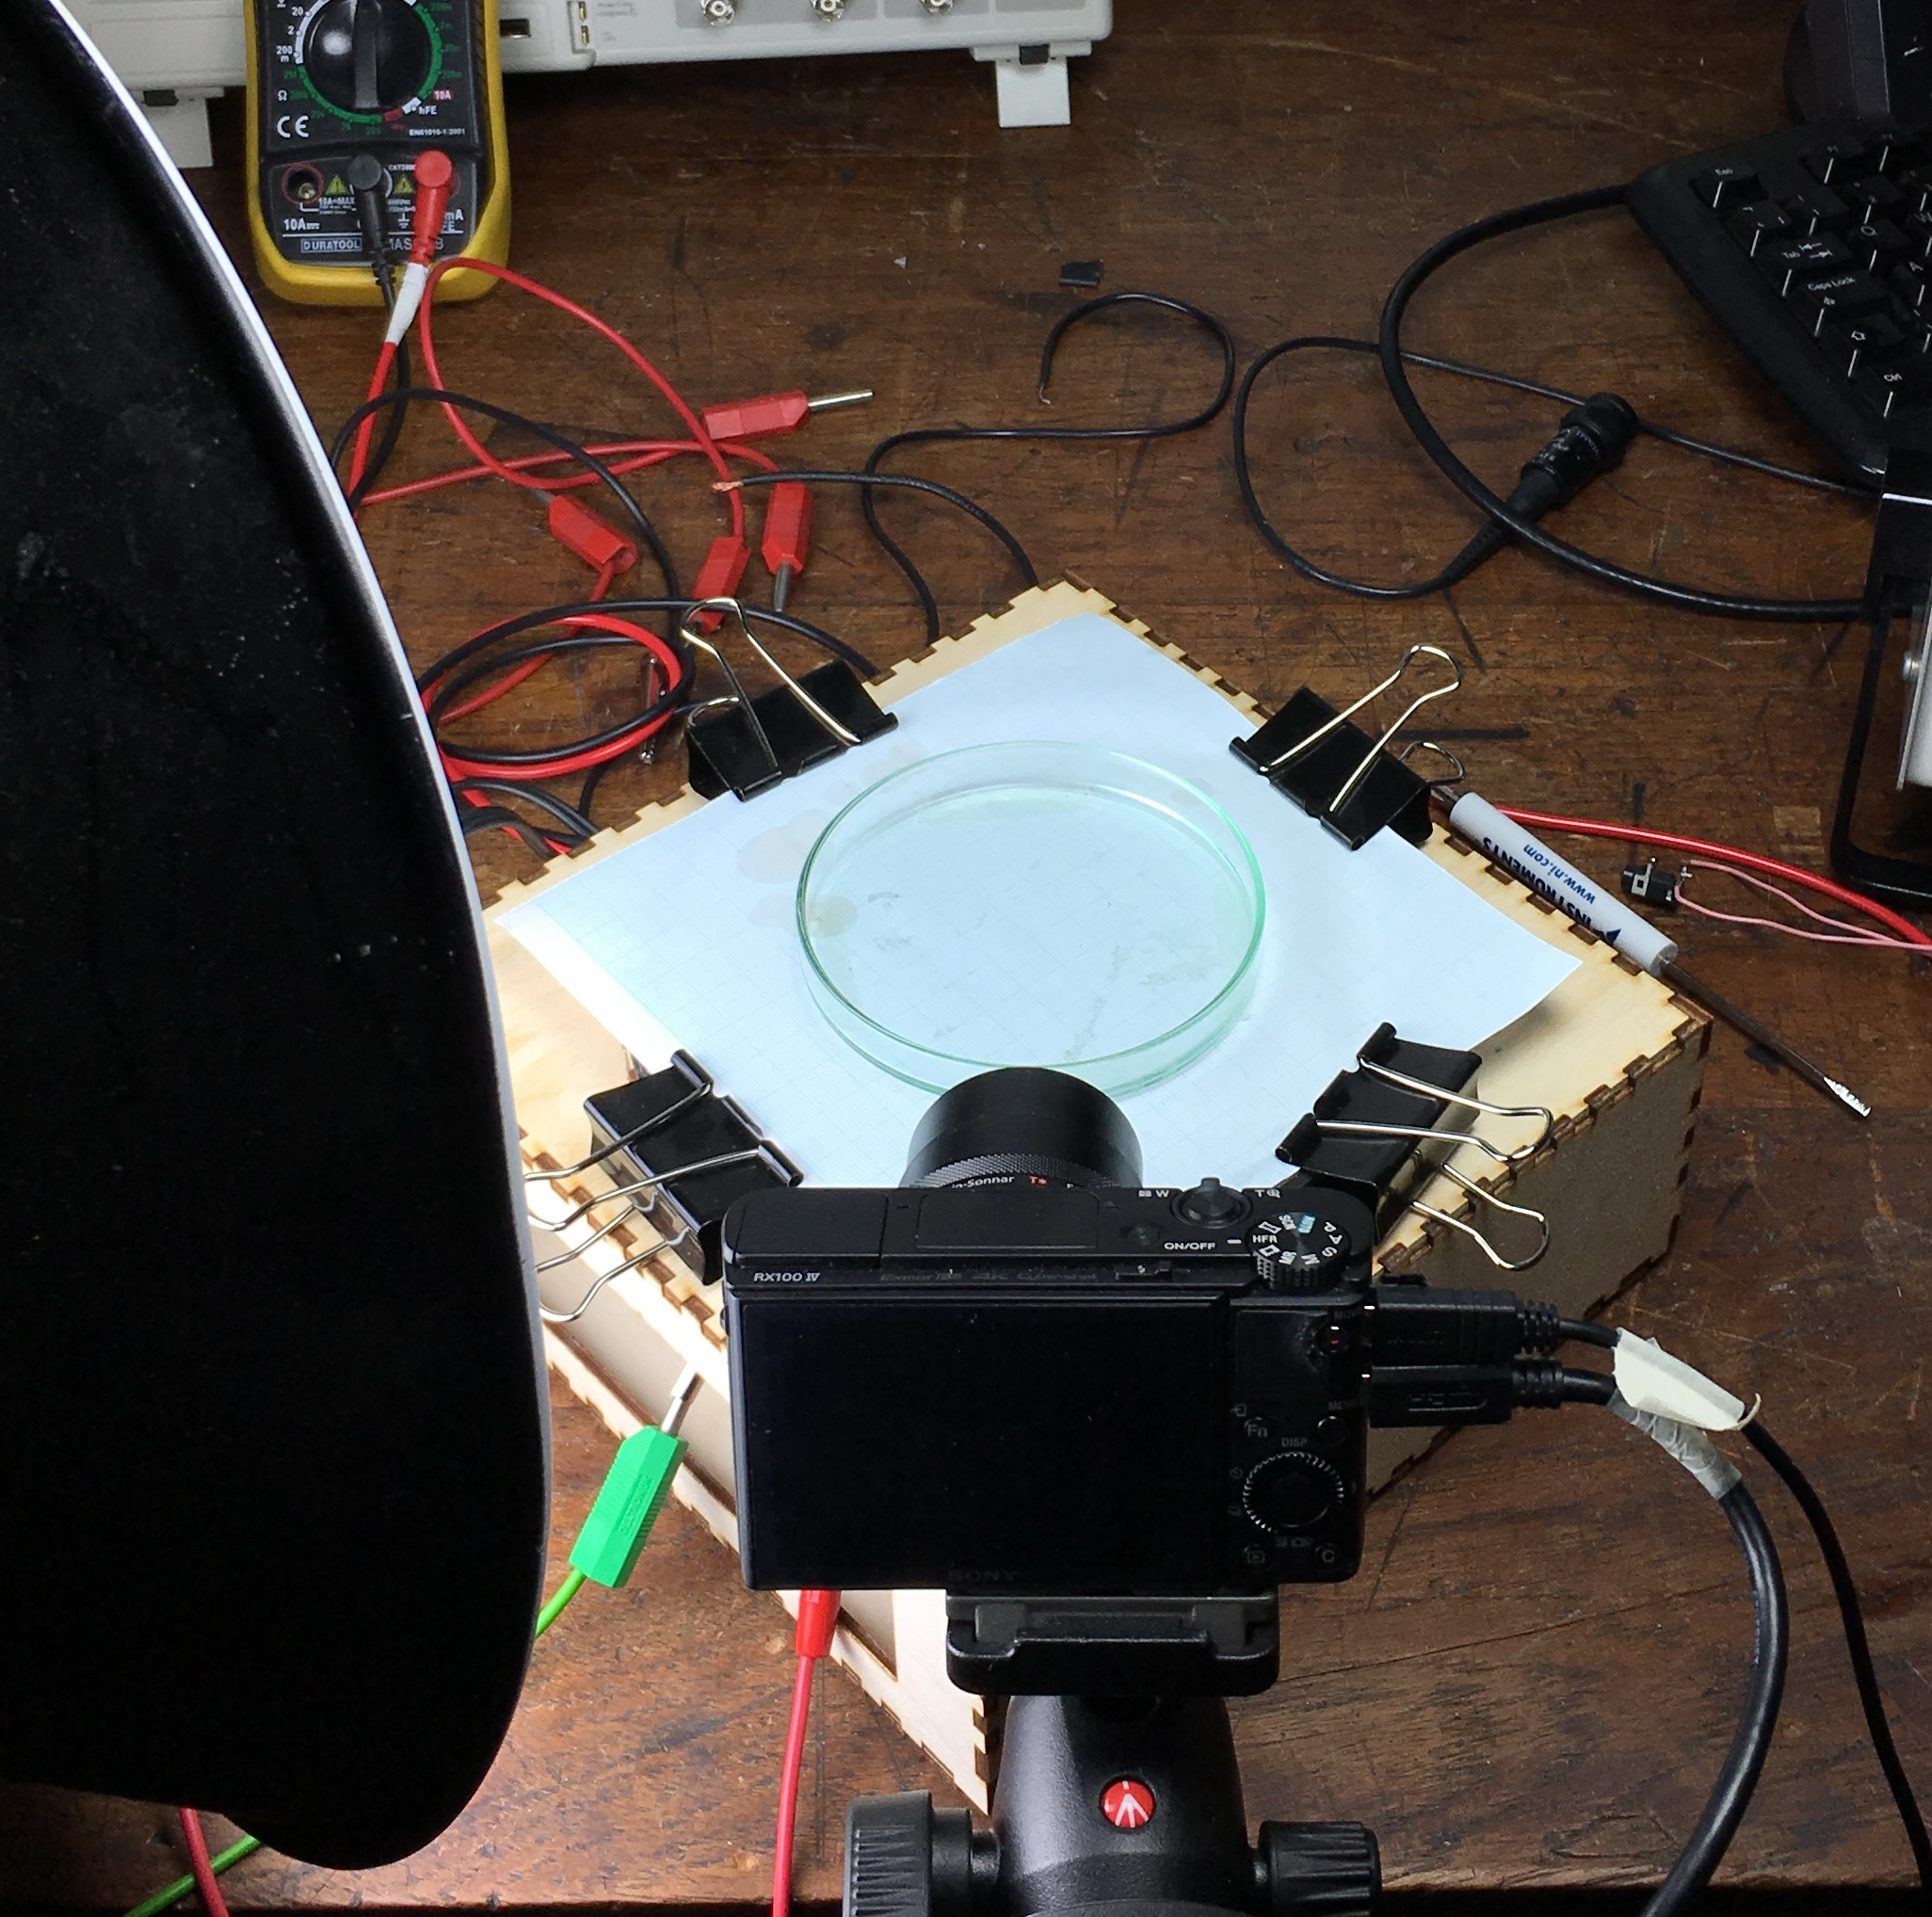
\includegraphics[width=\textwidth]{prototype/exp_rep_imgs/closeup_slowmo_setup.jpg}
        \caption{A closeup of the positioning of the camera and spotlight.}
    \end{subfigure}
    \begin{subfigure}[t]{0.475\textwidth}
    \centering
        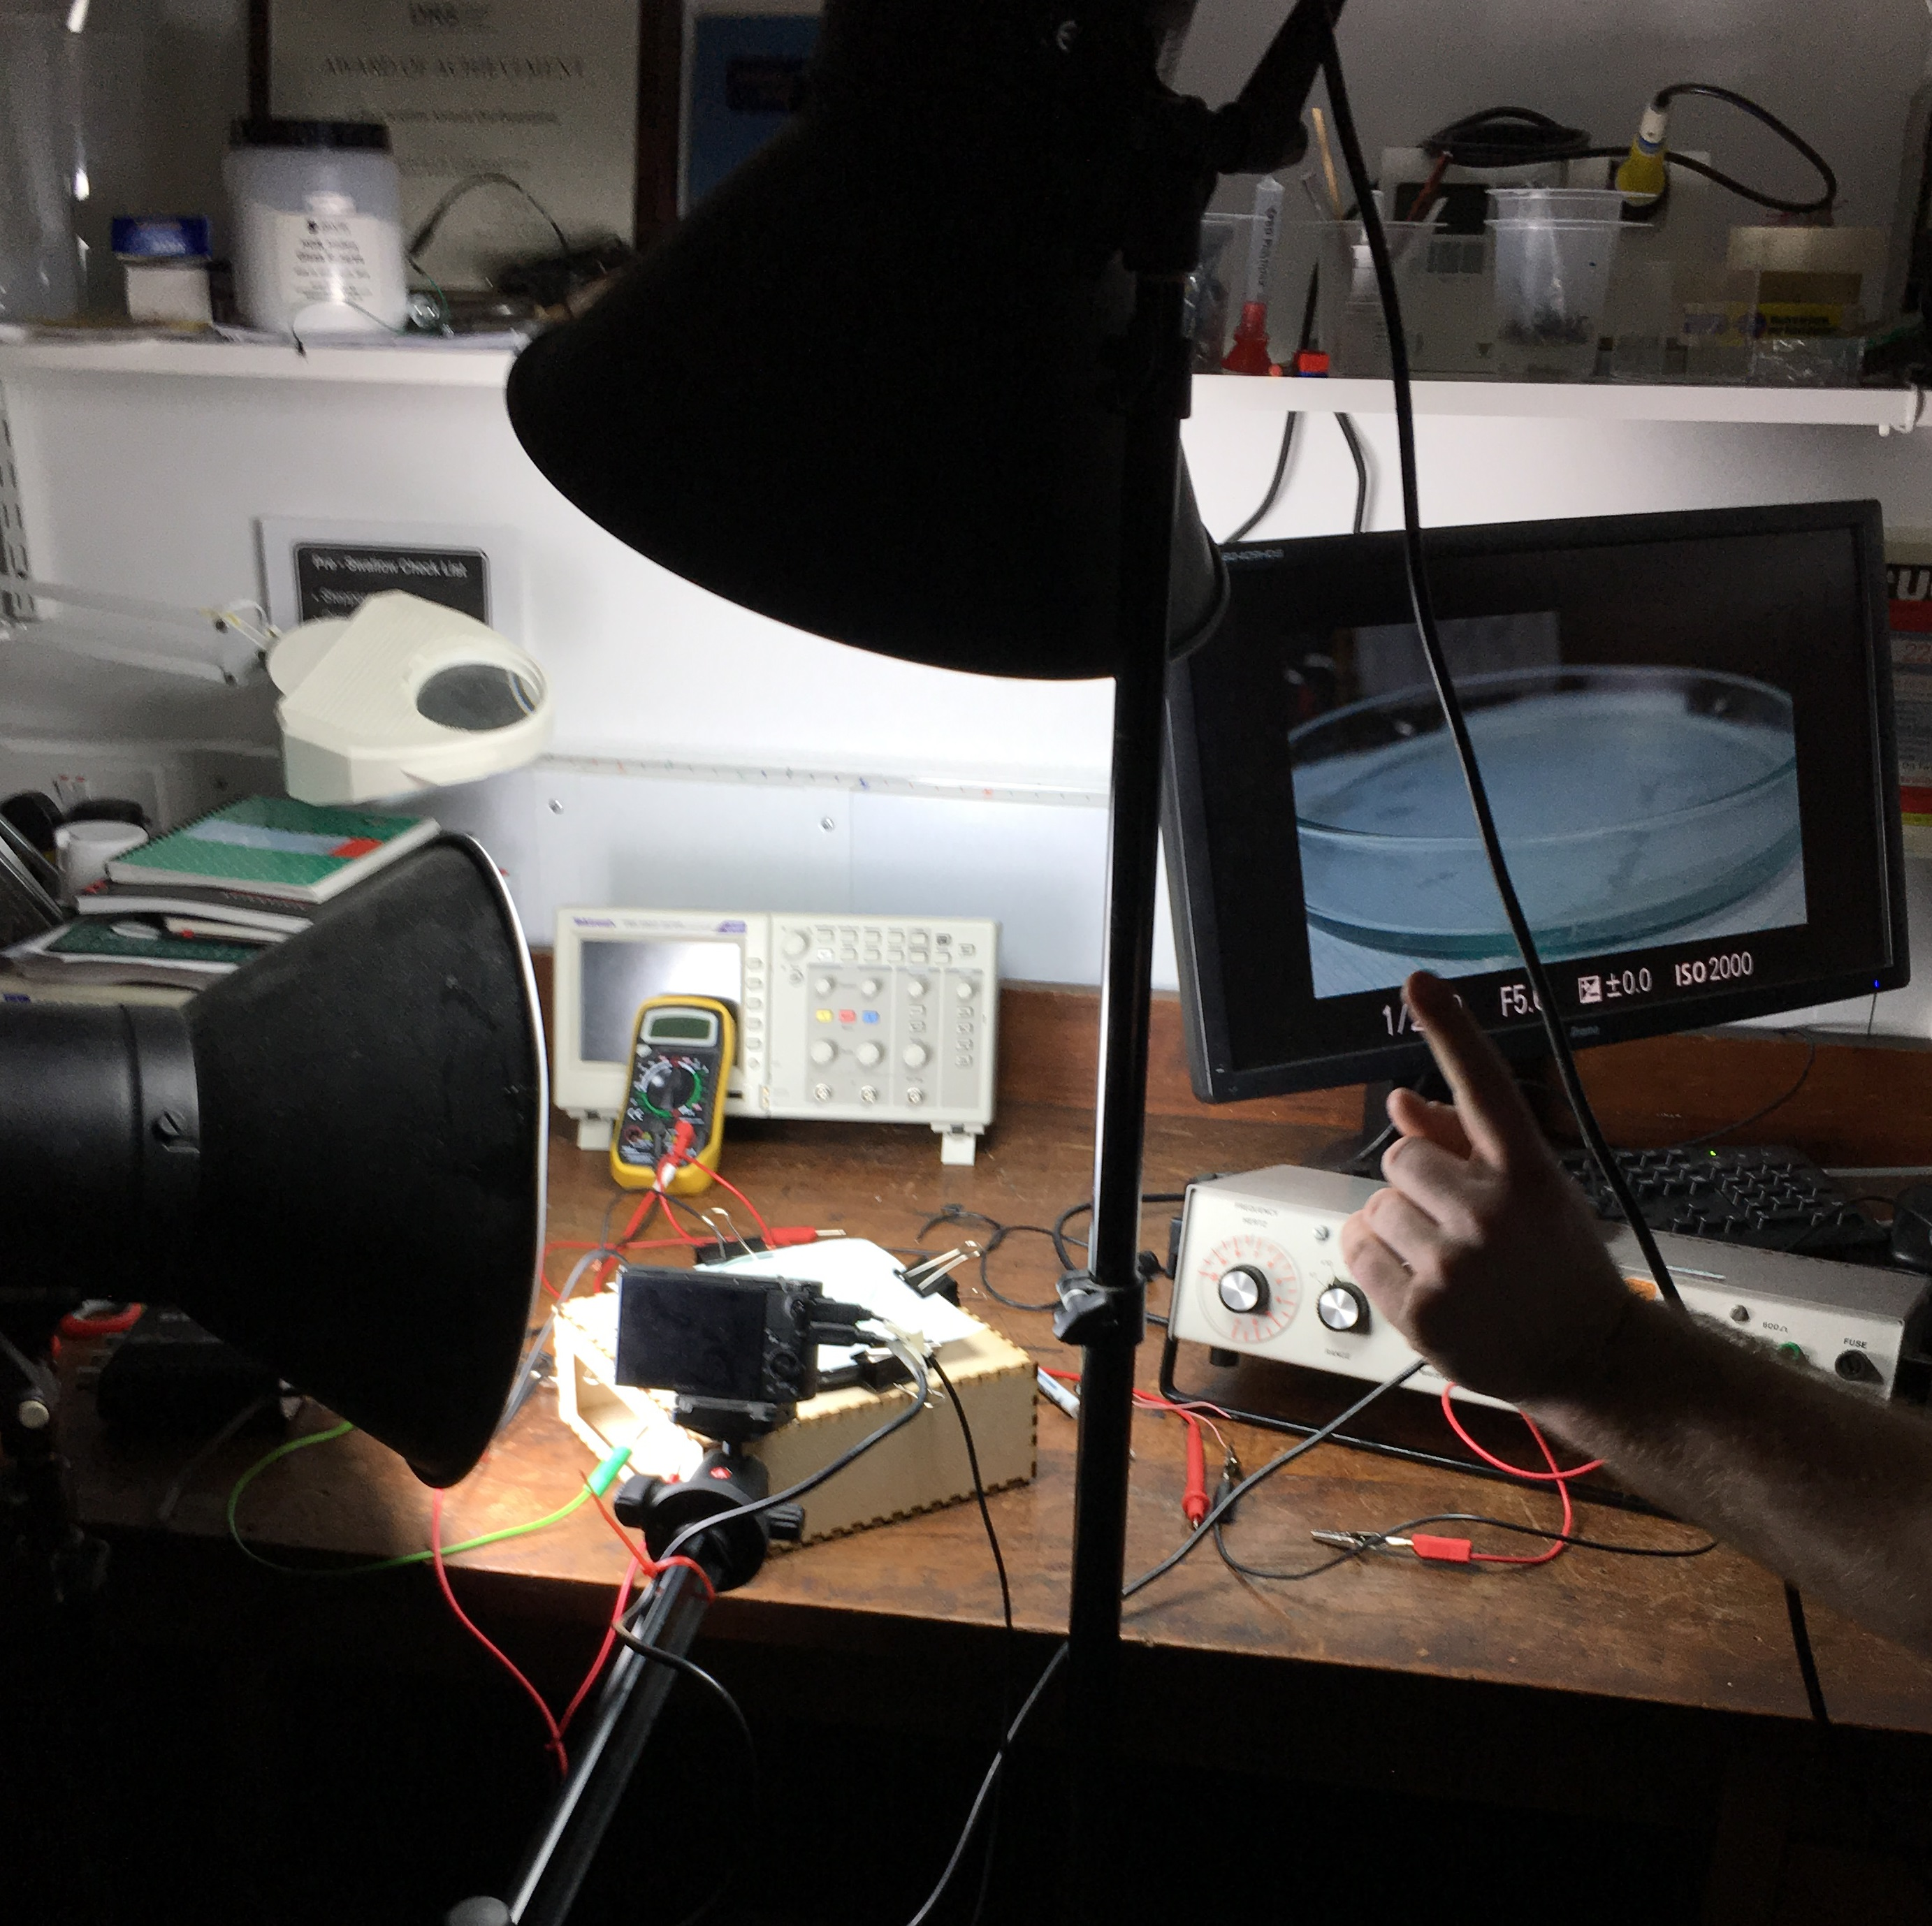
\includegraphics[width=\textwidth]{prototype/exp_rep_imgs/slowmo_setup.jpg}
        \caption{Full setup including the trigger and live recording on the computer monitor.}
    \end{subfigure}
\caption{The Sony Cyber-shot RX-100 IV Camera set up on a tripod, accompanied by spotlights for slow motion recording. }
\label{fig:slowmo_setup}
\end{figure}

Though the focusing was difficult at the start, it was resolved by forcing the droplets closer to the edge of the petri dish. Graph paper was taped underneath the petri dish to get an idea of the typical size of droplets. They were found to be approximately 1 mm in diameter. Recording was achieved at regular (25 fps) and high (50 fps) speeds through a frequency range of 50 -- 80 Hz. It was found that droplets were most stable at 50 Hz, which became the standard frequency used. As the strong lighting caused unwanted reflections, it was suggested that a polaroid or a diffuser be used to filter the light. This is analogous to wearing polarising sunglasses and being able to see fish in water more easily.

Interestingly, the bouncing itself was refracted through the glass and waves were observed on the bottom of the petri dish. This can be seen in Figure \ref{fig:bouncing_refr_glass}. Following this, research was carried out into the potential of motion tracking in obtaining quantitative data. It was found that Adobe AfterEffects offered this function. The method is summarised in the following steps:

\begin{enumerate}
\item  Creating a new null object to store the droplet coordinates
\item  Using the Track Camera, locate the region to track and then analyze  the clip.
\item  Apply the results to the null object.
\item  Select all key frames and paste in notepad.
\item  Plot in Excel.
\end{enumerate}

\begin{figure}[ht]
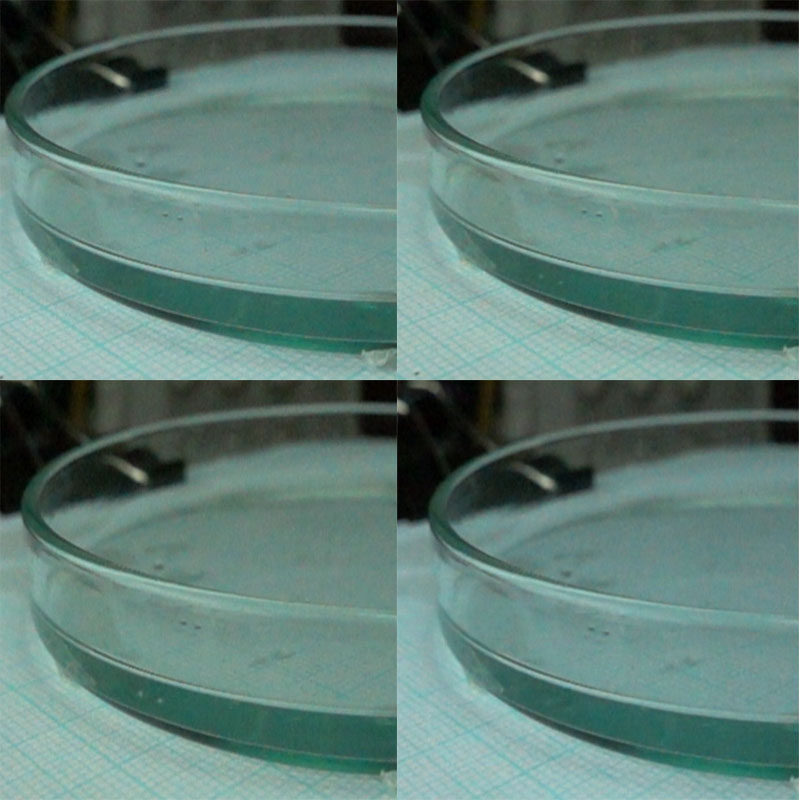
\includegraphics[width=\textwidth]{prototype/exp_rep_imgs/bouncing_refr_glass.jpg}
\centering
\caption{Four images displaying the bouncing motion refracted through the glass, captured using the Sony Cyber-shot RX-100 IV setup and 50 cSt silicone oil. With silicone oil, the droplets are hard to see, even with slow motion recording, due to their small size and transparent nature.}
\centering
\label{fig:bouncing_refr_glass}
\end{figure}

\subsection{Uncontrolled Experimental Factors}
During experimentation, attempts were made to observe walking and repelling pairs, in order to gain an idea of the typical amplifier volume needed to produce such phenomena. At the beginning, the temperature of the lab was measured. Low temperature led to a higher viscosity, which could have had an effect on droplet motion. Oil depth was also considered to be a factor.

Under normal lighting, the shadow of the droplet was projected on the graph paper when illuminated from above. This was used to obtain an estimate of the size of the droplet, although this was subject to parallax error as it had to be observed at an angle.

An attempt to determine the signal amplitude that created Faraday instability was made. A series of measurements of noise level were made at different distances for a fixed volume. This was to determine the sound level variation as a function of distance. The results were inconclusive, but it was decided that a fixed distance of 30 cm was to be used. Having a quantitative measure of noise level provided an alternative to measuring the acceleration. However, there was very little success in measuring the variation and a fixed noise level to achieve Faraday instability.

It was eventually decided that, due to the difficulty in trying to quantify measurements, it would be most effective to observe and record phenomena. This was deemed a path of greater success given the time frame for this project.

\subsection{Double slit diffraction}
Following these investigations, a resized plywood base was produced and fitted onto the loudspeaker with foldback clips. The use of tape was also eliminated as the clips were secure enough. Double slit diffraction was attempted by constructing a grating with rectangular wooden sticks. The petri dish was replaced with a square Tupperware box as shown in Figure \ref{fig:double_slit_setup} as it had a larger area and more flexibility with positioning the gratings. The width of slits was approximately equal to the size of the droplets.

\begin{figure}[h]
    \centering
    \begin{subfigure}{0.475\textwidth}
        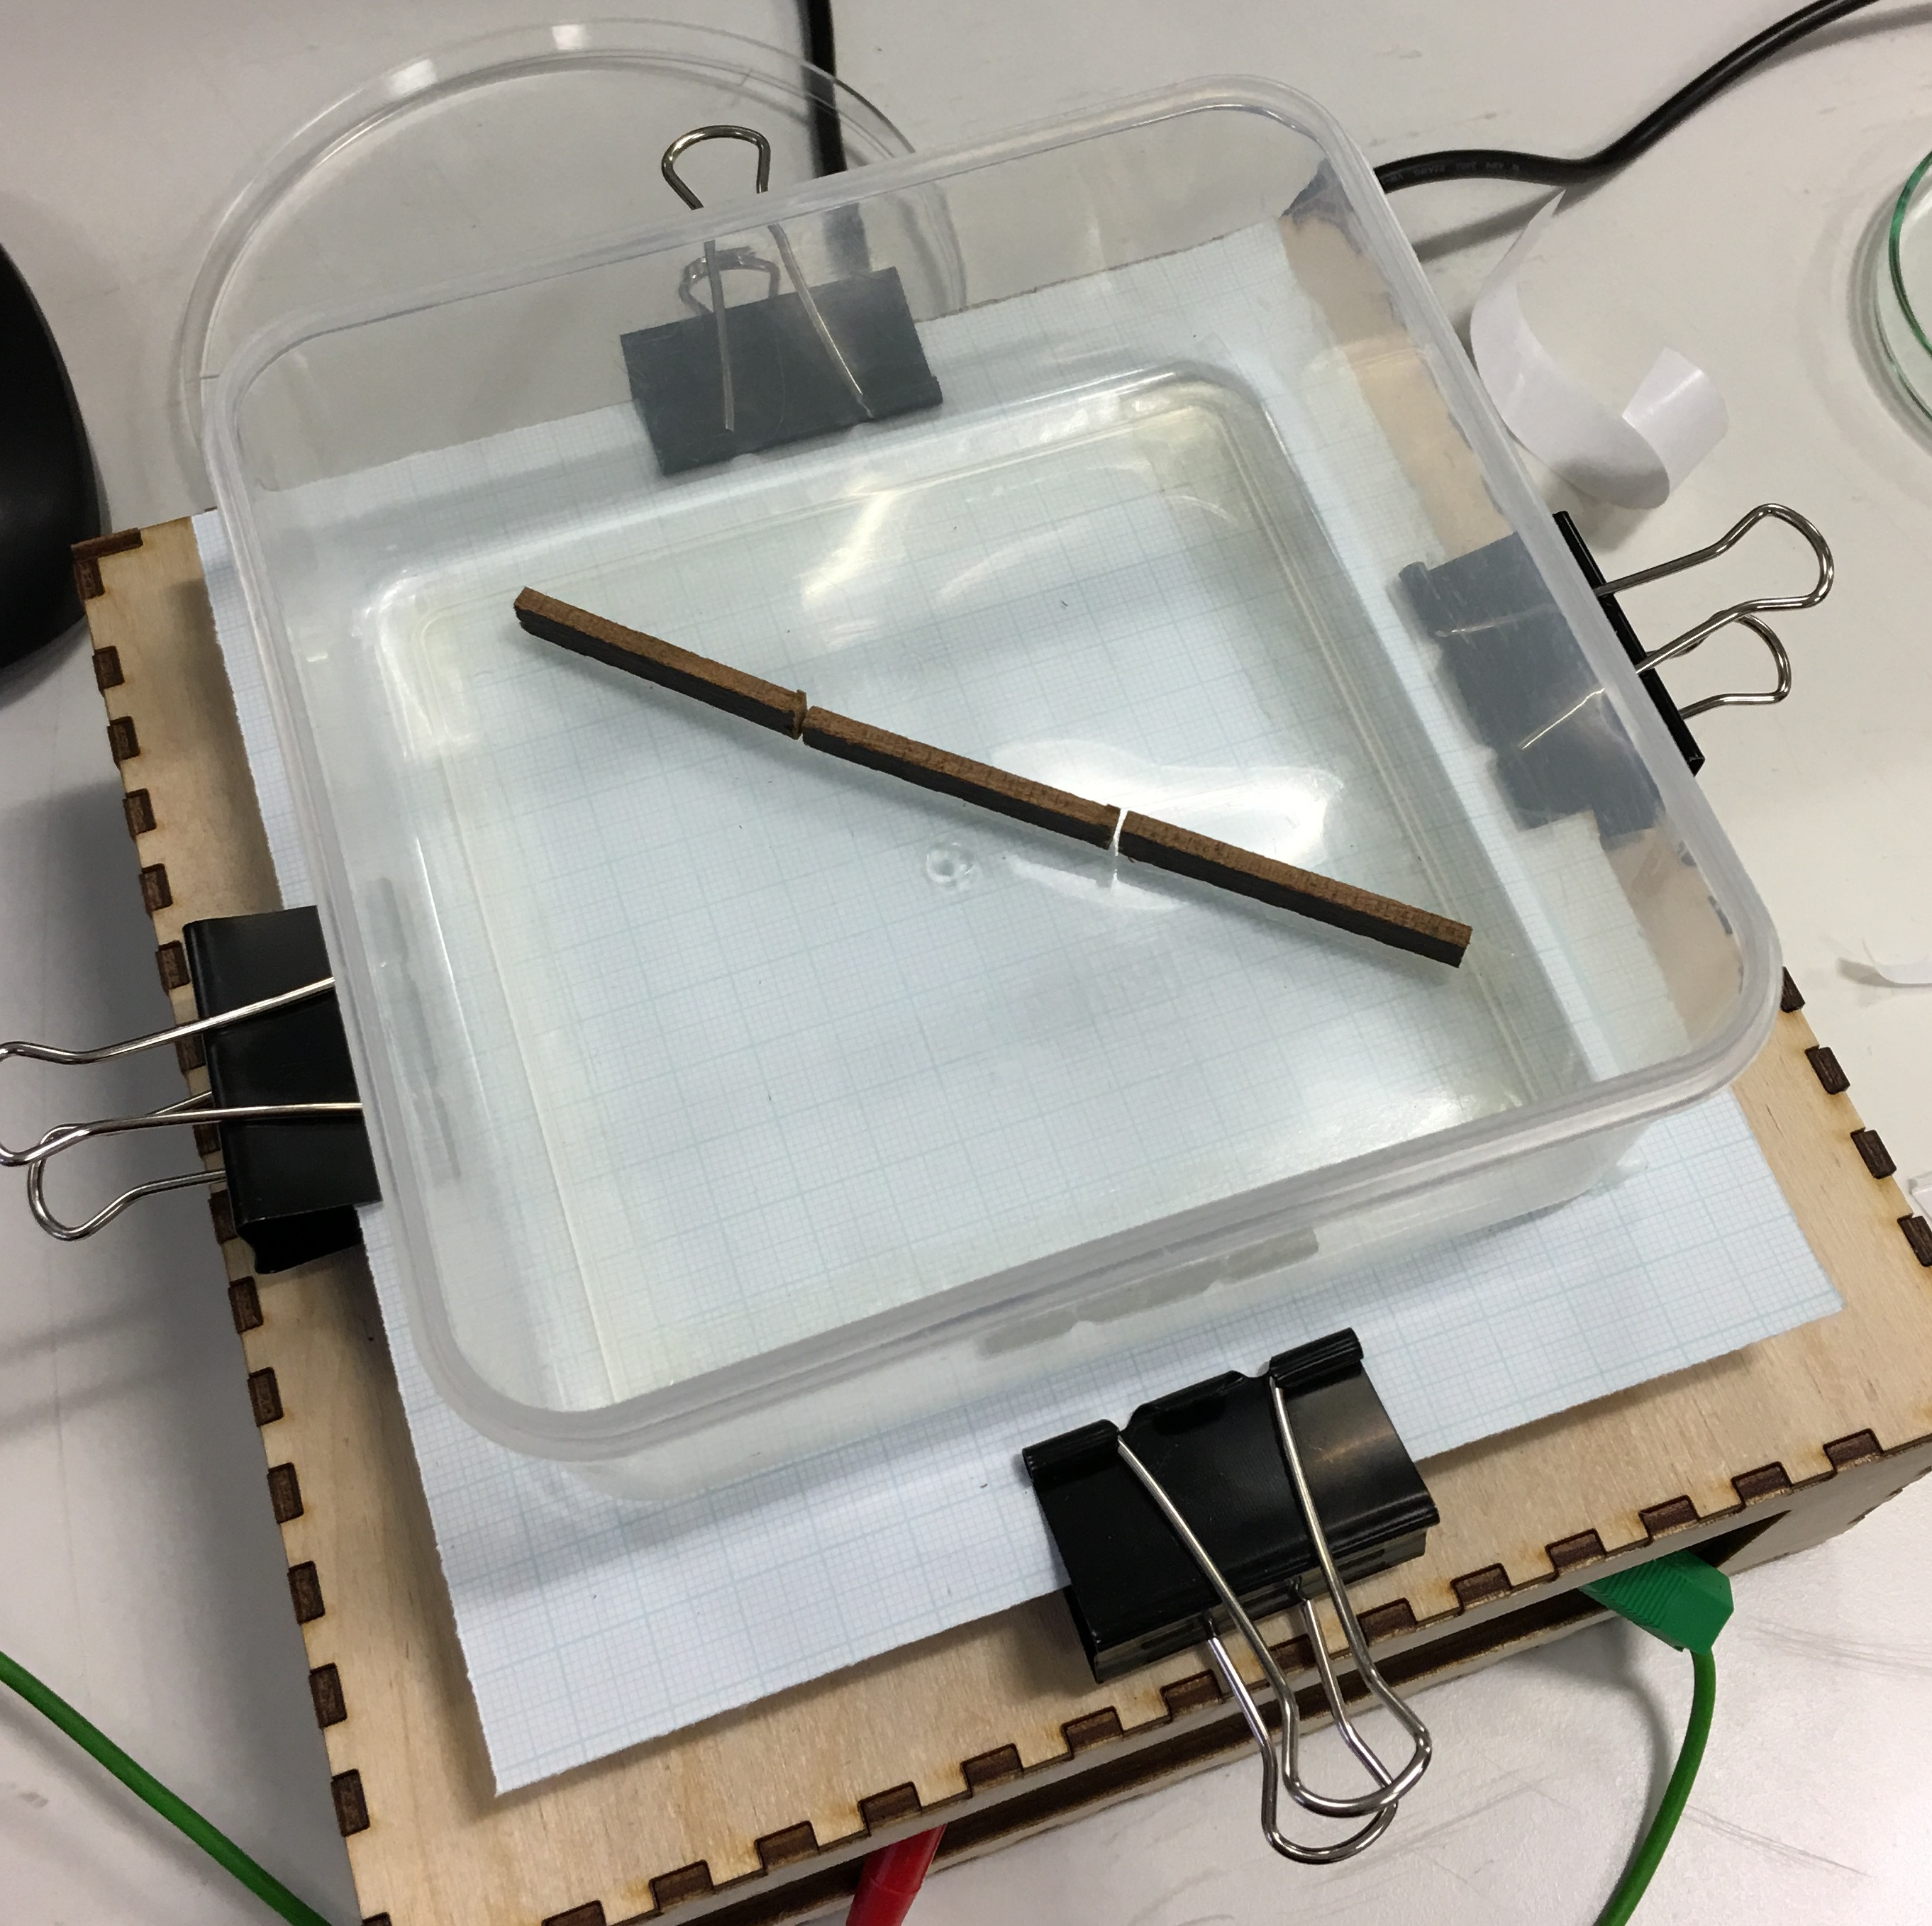
\includegraphics[width=\textwidth]{prototype/exp_rep_imgs/double_slit_setup_1.jpg}
        \caption{Double slit diffraction with slits located far from each other.}
    \end{subfigure}
    \begin{subfigure}{0.475\textwidth}
        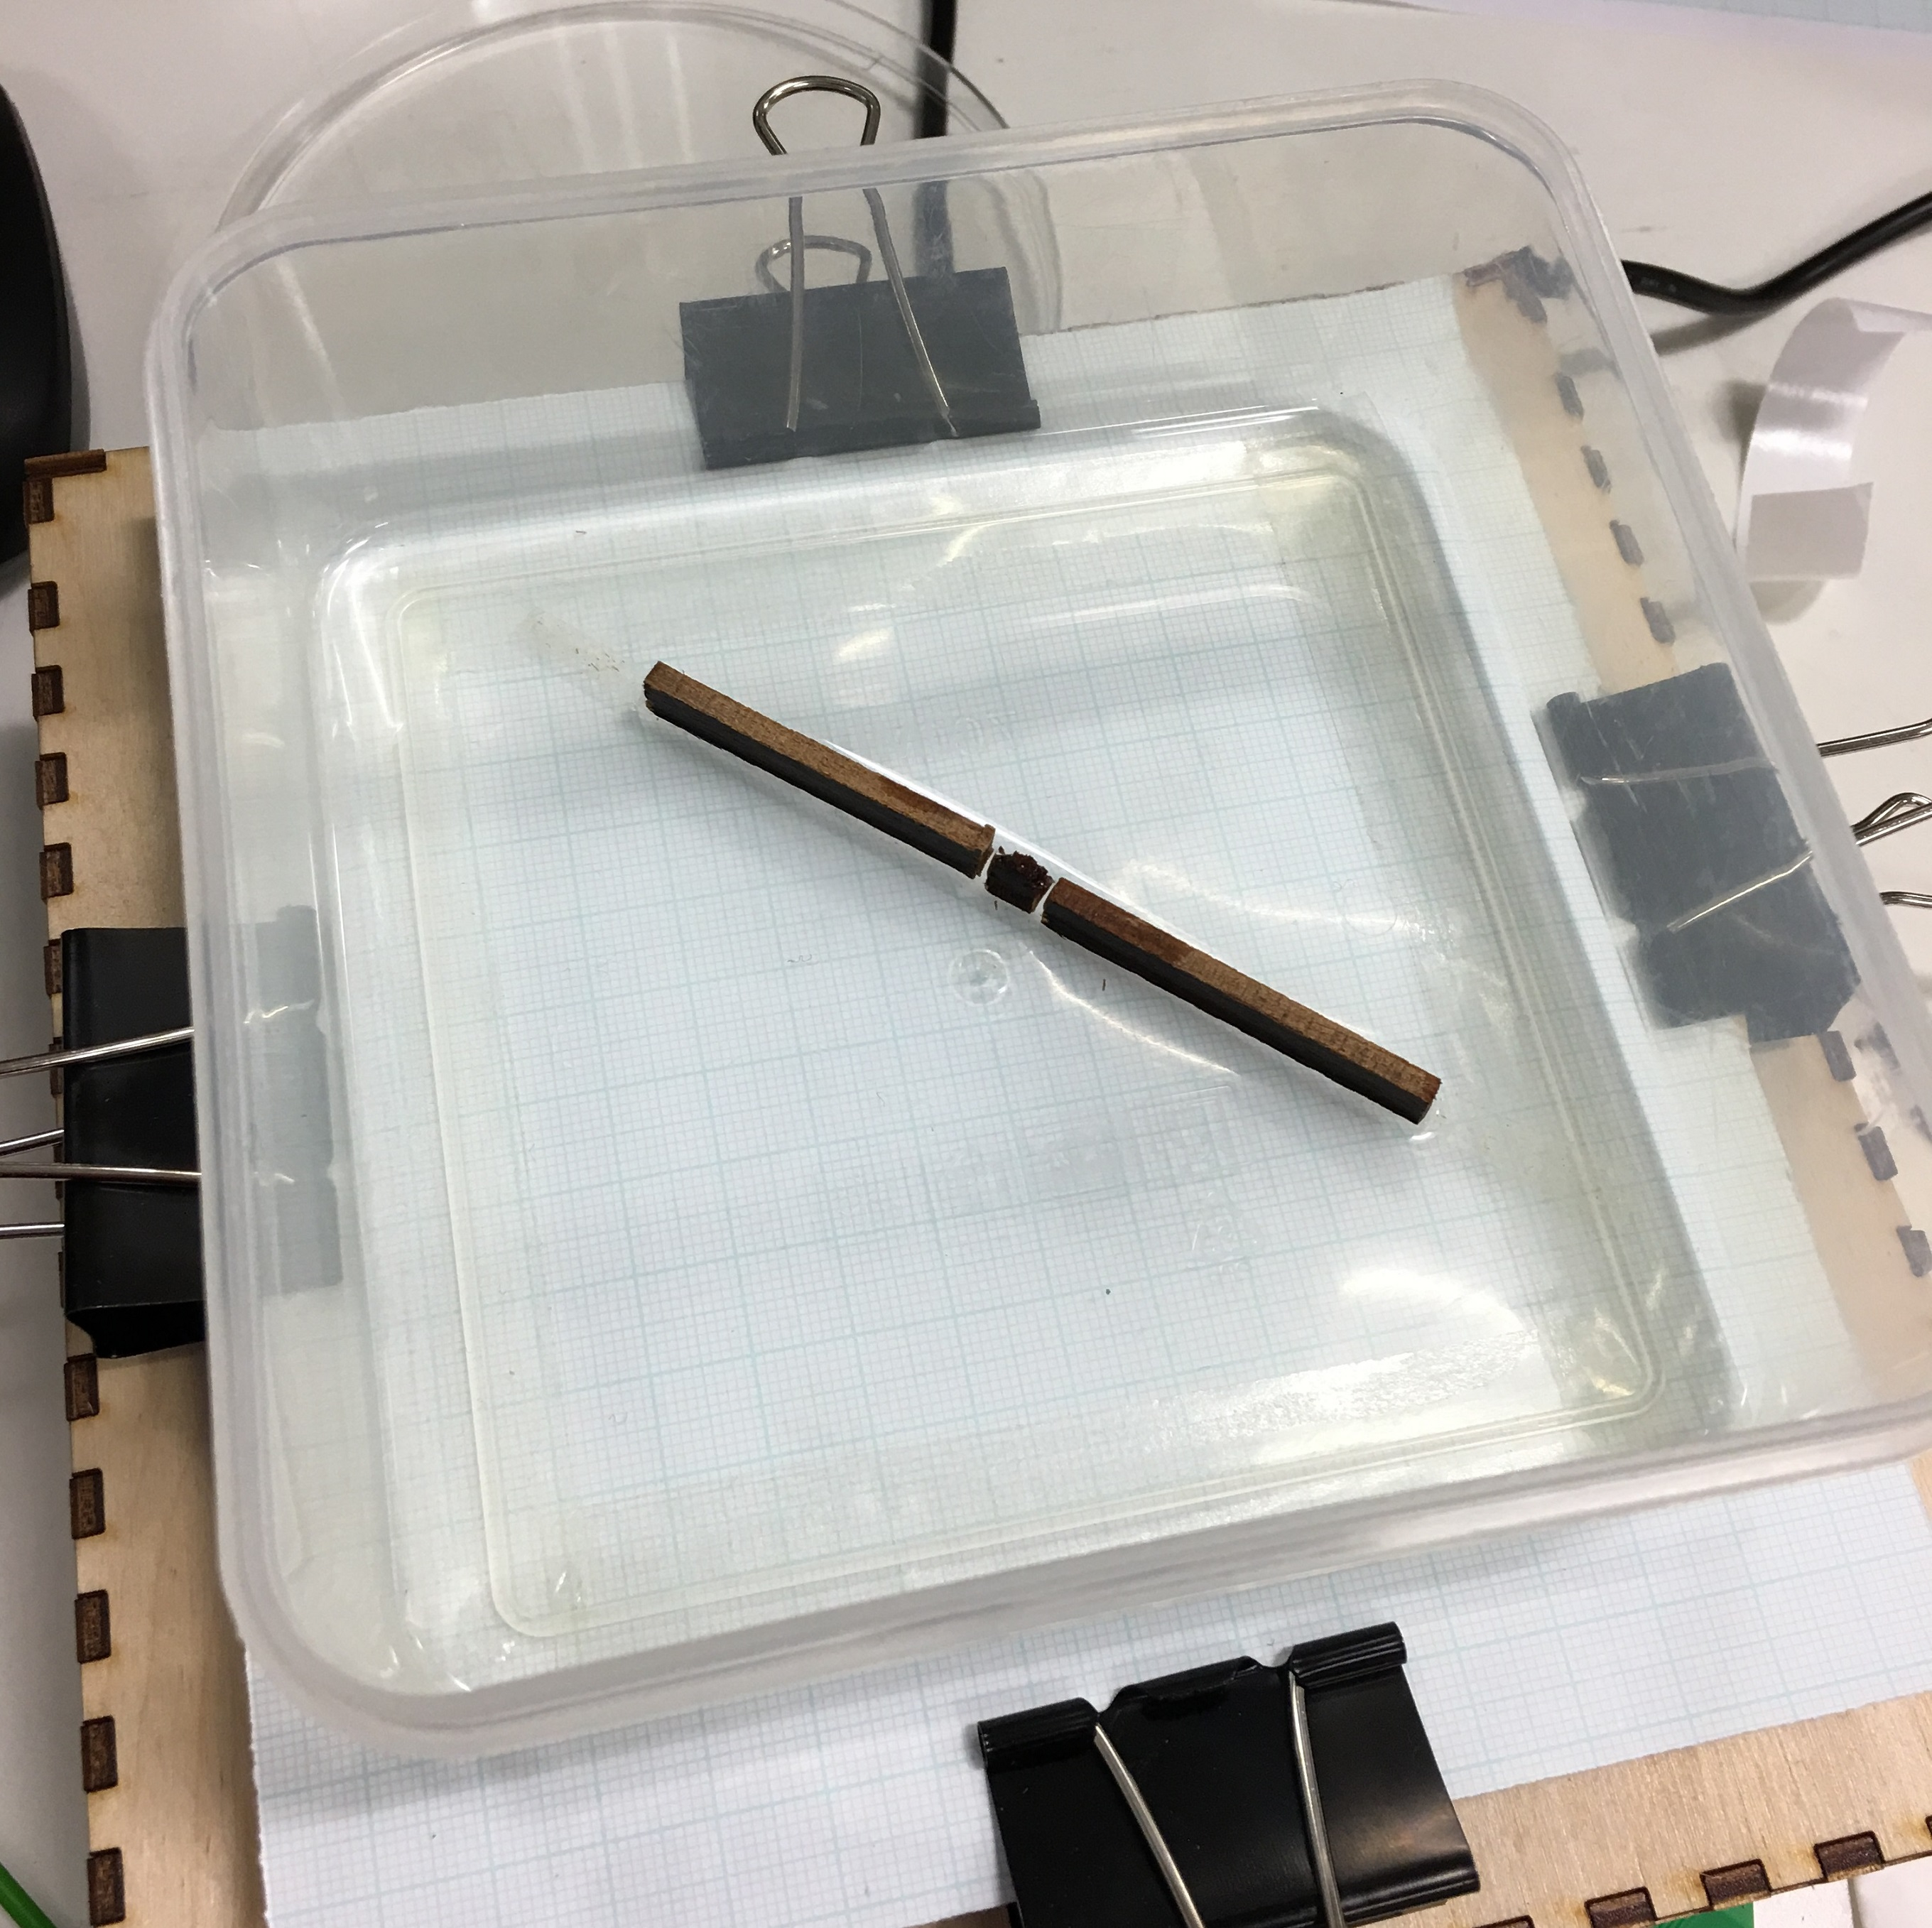
\includegraphics[width=\textwidth]{prototype/exp_rep_imgs/double_slit_setup_2.jpg}
        \caption{Double slit diffraction with both slits located near to each other.}
    \end{subfigure}
\caption{Images of the experimental setup used to try and capture double slit diffraction. A plastic Tupperware box was used in place of a petri dish. }
\label{fig:double_slit_setup}
\end{figure}

By producing droplets and forcing them towards the slits using compressed air, it was found that the silicone oil would crawl up the slit due to surface tension. The tension created a barrier which prevented the droplets from passing through the slit. This led to the use of more extreme methods, such as pushing the droplets with a wooden stick and even tilting the entire box at a large inclination. Both methods proved to be ineffective in overcoming the surface tension.

A proposed solution was to submerge the slits and push the droplets through. No visible diffraction was observed. Eventually the experiment was simplified and reverted to a single slit in a petri dish, where both submerged and non-submerged slits were tested. The same issue with surface tension was encountered, and again no diffraction was observed with the naked eye.

\subsection{Changing Fluid}
With a stable bouncing state achieved, it was decided that a different type of liquid should be tested. This time the experiment was carried out with washing up liquid diluted in water, as research papers have stated that soap water was one of the earliest liquids used to test the pilot-wave theory \cite{protiere2006particle}. It also is a good candidate if the project were to be commercialised or used as an educational tool in schools. The other candidate shortlisted was vegetable oil, as it has a similar viscosity with our previous silicone oil of 50 cSt, but widely available.

The soap water was produced by mixing washing liquid with water and stirring it with a wooden stick. At 50 Hz waves were much more visible due to the green tint from the washing up liquid; it was also predicted that the low viscosity of the liquid would help to produce more stable droplets. At a certain angle, waves produced by the droplets were clearly visible under ambient light.

The Faraday instability regime, a sudden increase in chaotic wave forms on the liquid surface, was also explored. The breaking of the surface also created chaotic motion of droplets, whereby they undergo irregular movements across the surface. By decreasing the amplitude under the Faraday threshold, the surface became calm again, and the only waves visible were the standing waves formed by the bouncing droplets. This was clearly visualised using the soap water as seen in Figure \ref{fig:faraday_inst_regime}.

\begin{figure}[htb]
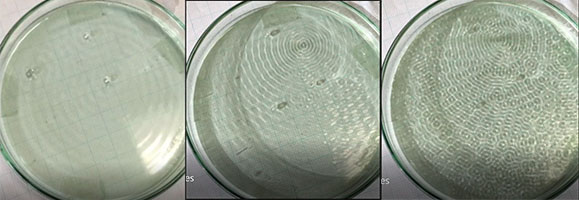
\includegraphics[width=\textwidth]{prototype/exp_rep_imgs/Faraday_inst_regime.jpg}
\centering
\caption{A series of images showing the evolution of a system to the Faraday instability regime, represented with the right-most image. The middle image represents the Faraday threshold, and the leftmost image is the regime where standing waves are formed by bouncing droplets. The diluted soap water produced a green tint.}
\centering
\label{fig:faraday_inst_regime}
\end{figure}

The new liquid also proved to be extremely effective in producing other phenomena that were not possible under silicone oil. Phenomena such as walking and orbiting were also observed and recorded, and Figure \ref{fig:orbit_droplets_interaction} shows an orbiting pair of similar sized droplets. It  was possible to sustain these for around 10 seconds before one is destroyed. Walking can be seen from Figure \ref{fig:double_slit_walking_perimeter}, where a droplet was observed to glide along the edge of the petri dish for many revolutions at a relatively fast speed. In this image, plastic slits were used to test double slit diffraction again. However, surface tension still arose, which motivated a change in technique. The slits were moved towards the droplets instead, the relative motion was thought to produce a similar effect. However, the effects were not visible with the naked eye.

\begin{figure}[htb]
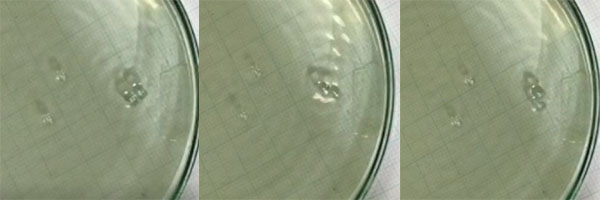
\includegraphics[width=\textwidth]{prototype/exp_rep_imgs/orbit_droplets_interaction.jpg}
\centering
\caption{A series of images showing an orbiting pair of similar sized droplets. Two other bouncing droplets can also be seen in the left.}
\centering
\label{fig:orbit_droplets_interaction}
\end{figure}

\begin{figure}[htb]
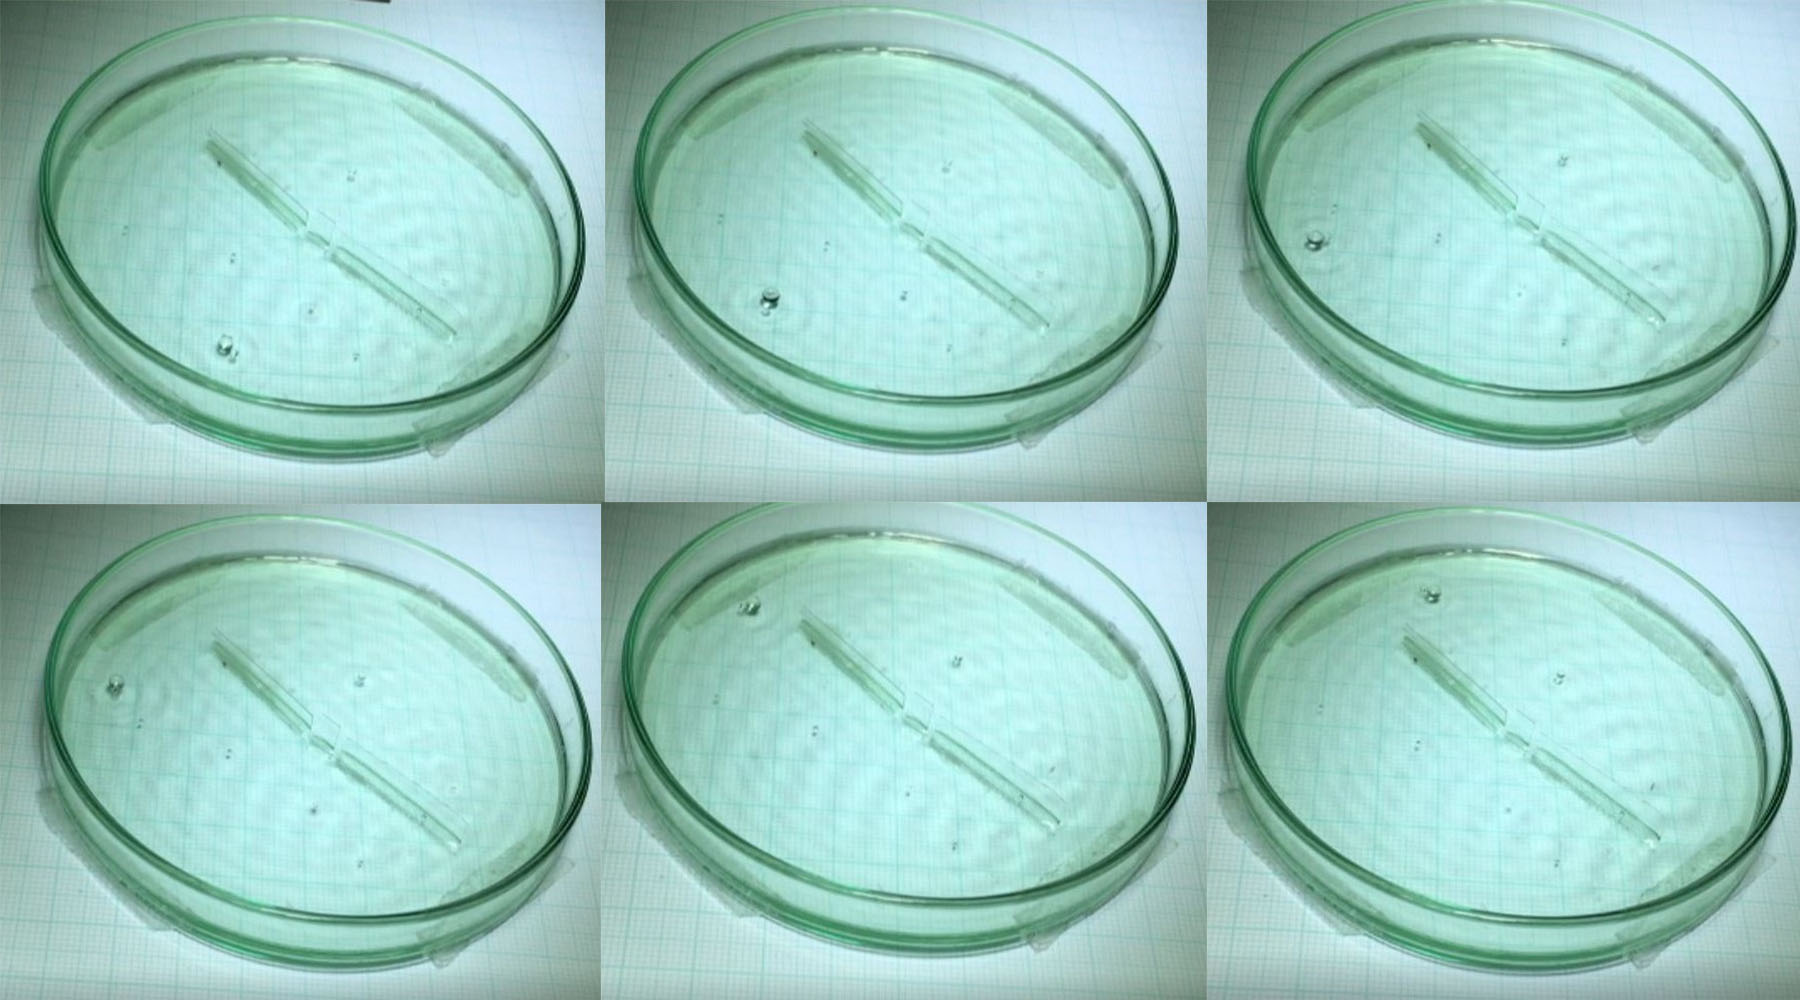
\includegraphics[width=\textwidth]{prototype/exp_rep_imgs/double_slit_walking_perimeter.jpg}
\centering
\caption{A series of images displaying the motion of a walking droplet around the perimeter of the petri dish. The droplet was observed to travel for several rounds before coalescing.}
\centering
\label{fig:double_slit_walking_perimeter}
\end{figure}

As a  result of using soap water, more consistent droplets were created and more quantum phenomena were observed. Another observation included a cluster that resembles a crystalline lattice structure, where three droplets formed a triangular lattice as shown in Figure \ref{fig:triangle_structure}. A bigger cluster formed an irregular lattice that can be seen in Figure \ref{fig:irregular_structure}.

\begin{figure}[ht]
    \begin{subfigure}[t]{0.5\textwidth}
        \centering
        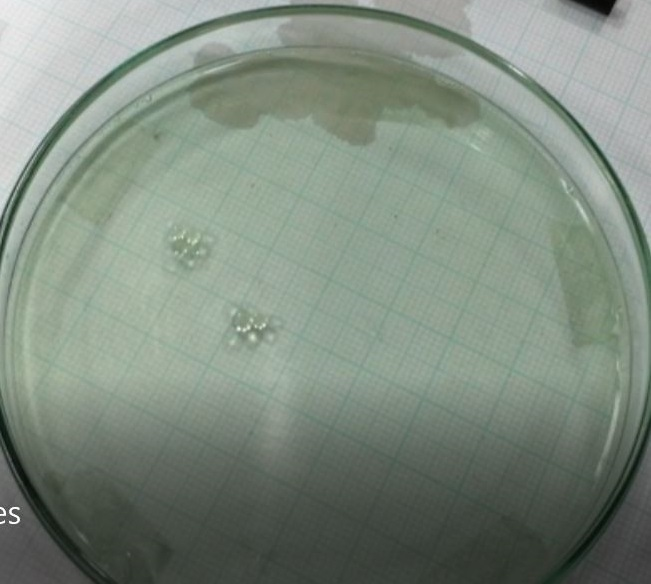
\includegraphics[width=\textwidth]{prototype/exp_rep_imgs/triangular_lattice.jpg}
        \caption{An aggregate of three droplets, formed from the self-assembly of steady state bouncers into a cluster}
        \label{fig:triangle_structure}
    \end{subfigure}
    \begin{subfigure}[t]{0.5\textwidth}
        \centering
        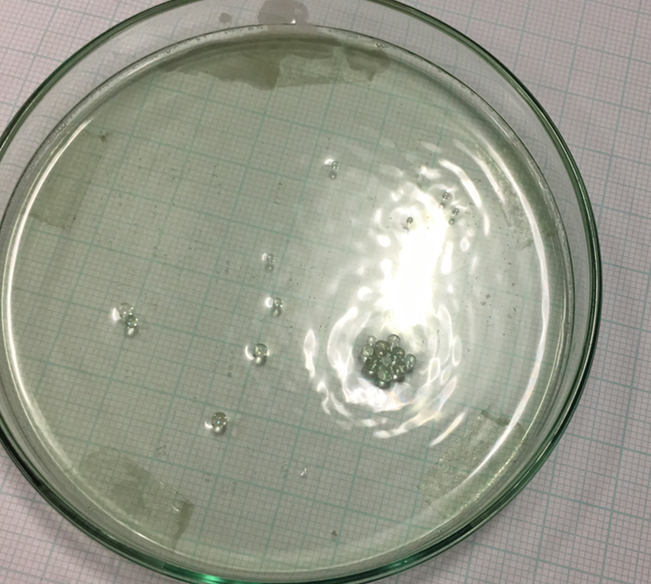
\includegraphics[width=\textwidth]{prototype/exp_rep_imgs/lattice_cluster.jpg}
        \caption{A larger cluster of droplets. They did not form a regular crystalline lattice structure, rather a random assembly. It was observed that droplets would tend towards each other regardless of their initial starting position}
        \label{fig:irregular_structure}
    \end{subfigure}
\caption{Crystalline lattice structures formed by steady state bouncing droplets.}
\label{fig:irregular_structure_evolution}
\end{figure}


To wrap up, food colouring was used to try and enhance visualisation. The result can be seen in Figure \ref{fig:red_dye}. A repelling quadruple was observed. This was predicted by how droplets were in anti-phase when they were in the bound state. If they were in phase, the resultant phenomenon would be the orbiting state.

\begin{figure}[ht]
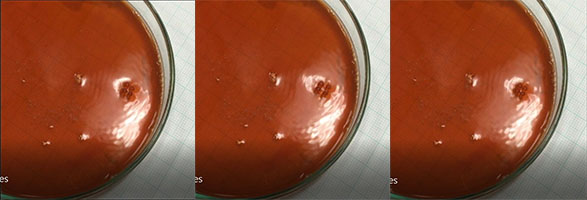
\includegraphics[width=\textwidth]{prototype/exp_rep_imgs/red_dye.jpg}
\centering
\caption{Repelling quadruple droplets with soap water dyed red. This is a much more complex motion due to having four bound droplets. Other than repelling, the droplets were also observed to behave like a viscous liquid.}
\centering
\label{fig:red_dye}
\end{figure}

\subsection{Ultra High Speed Camera}
A high speed camera (Photron Fastcam SA1.1) with the capability to record up to 675,000 fps was rented from the Department of Chemical Engineering, supervised by Dr. Han Wu. This was accompanied with a pair of table-attachable high power  lights, a regular camera for recording at a normal rate (25 fps), a diffuser, and a laptop with the software required to operate the high speed camera. It was discovered that the camera can only record in black and white.

An issue arose when attempting to find the best angle and distance for the camera to have the best focus; positioning the spotlight and adjusting the aperture were necessary to better visualise the final image on the computer.

In this attempt, plastic slits were superglued to the petri dish to attempt diffraction with soap water, although it was uncertain how the glue would have mixed with the soap. The slits are shown in Figure \ref{fig:plastic_slits}.

\begin{figure}[htb]
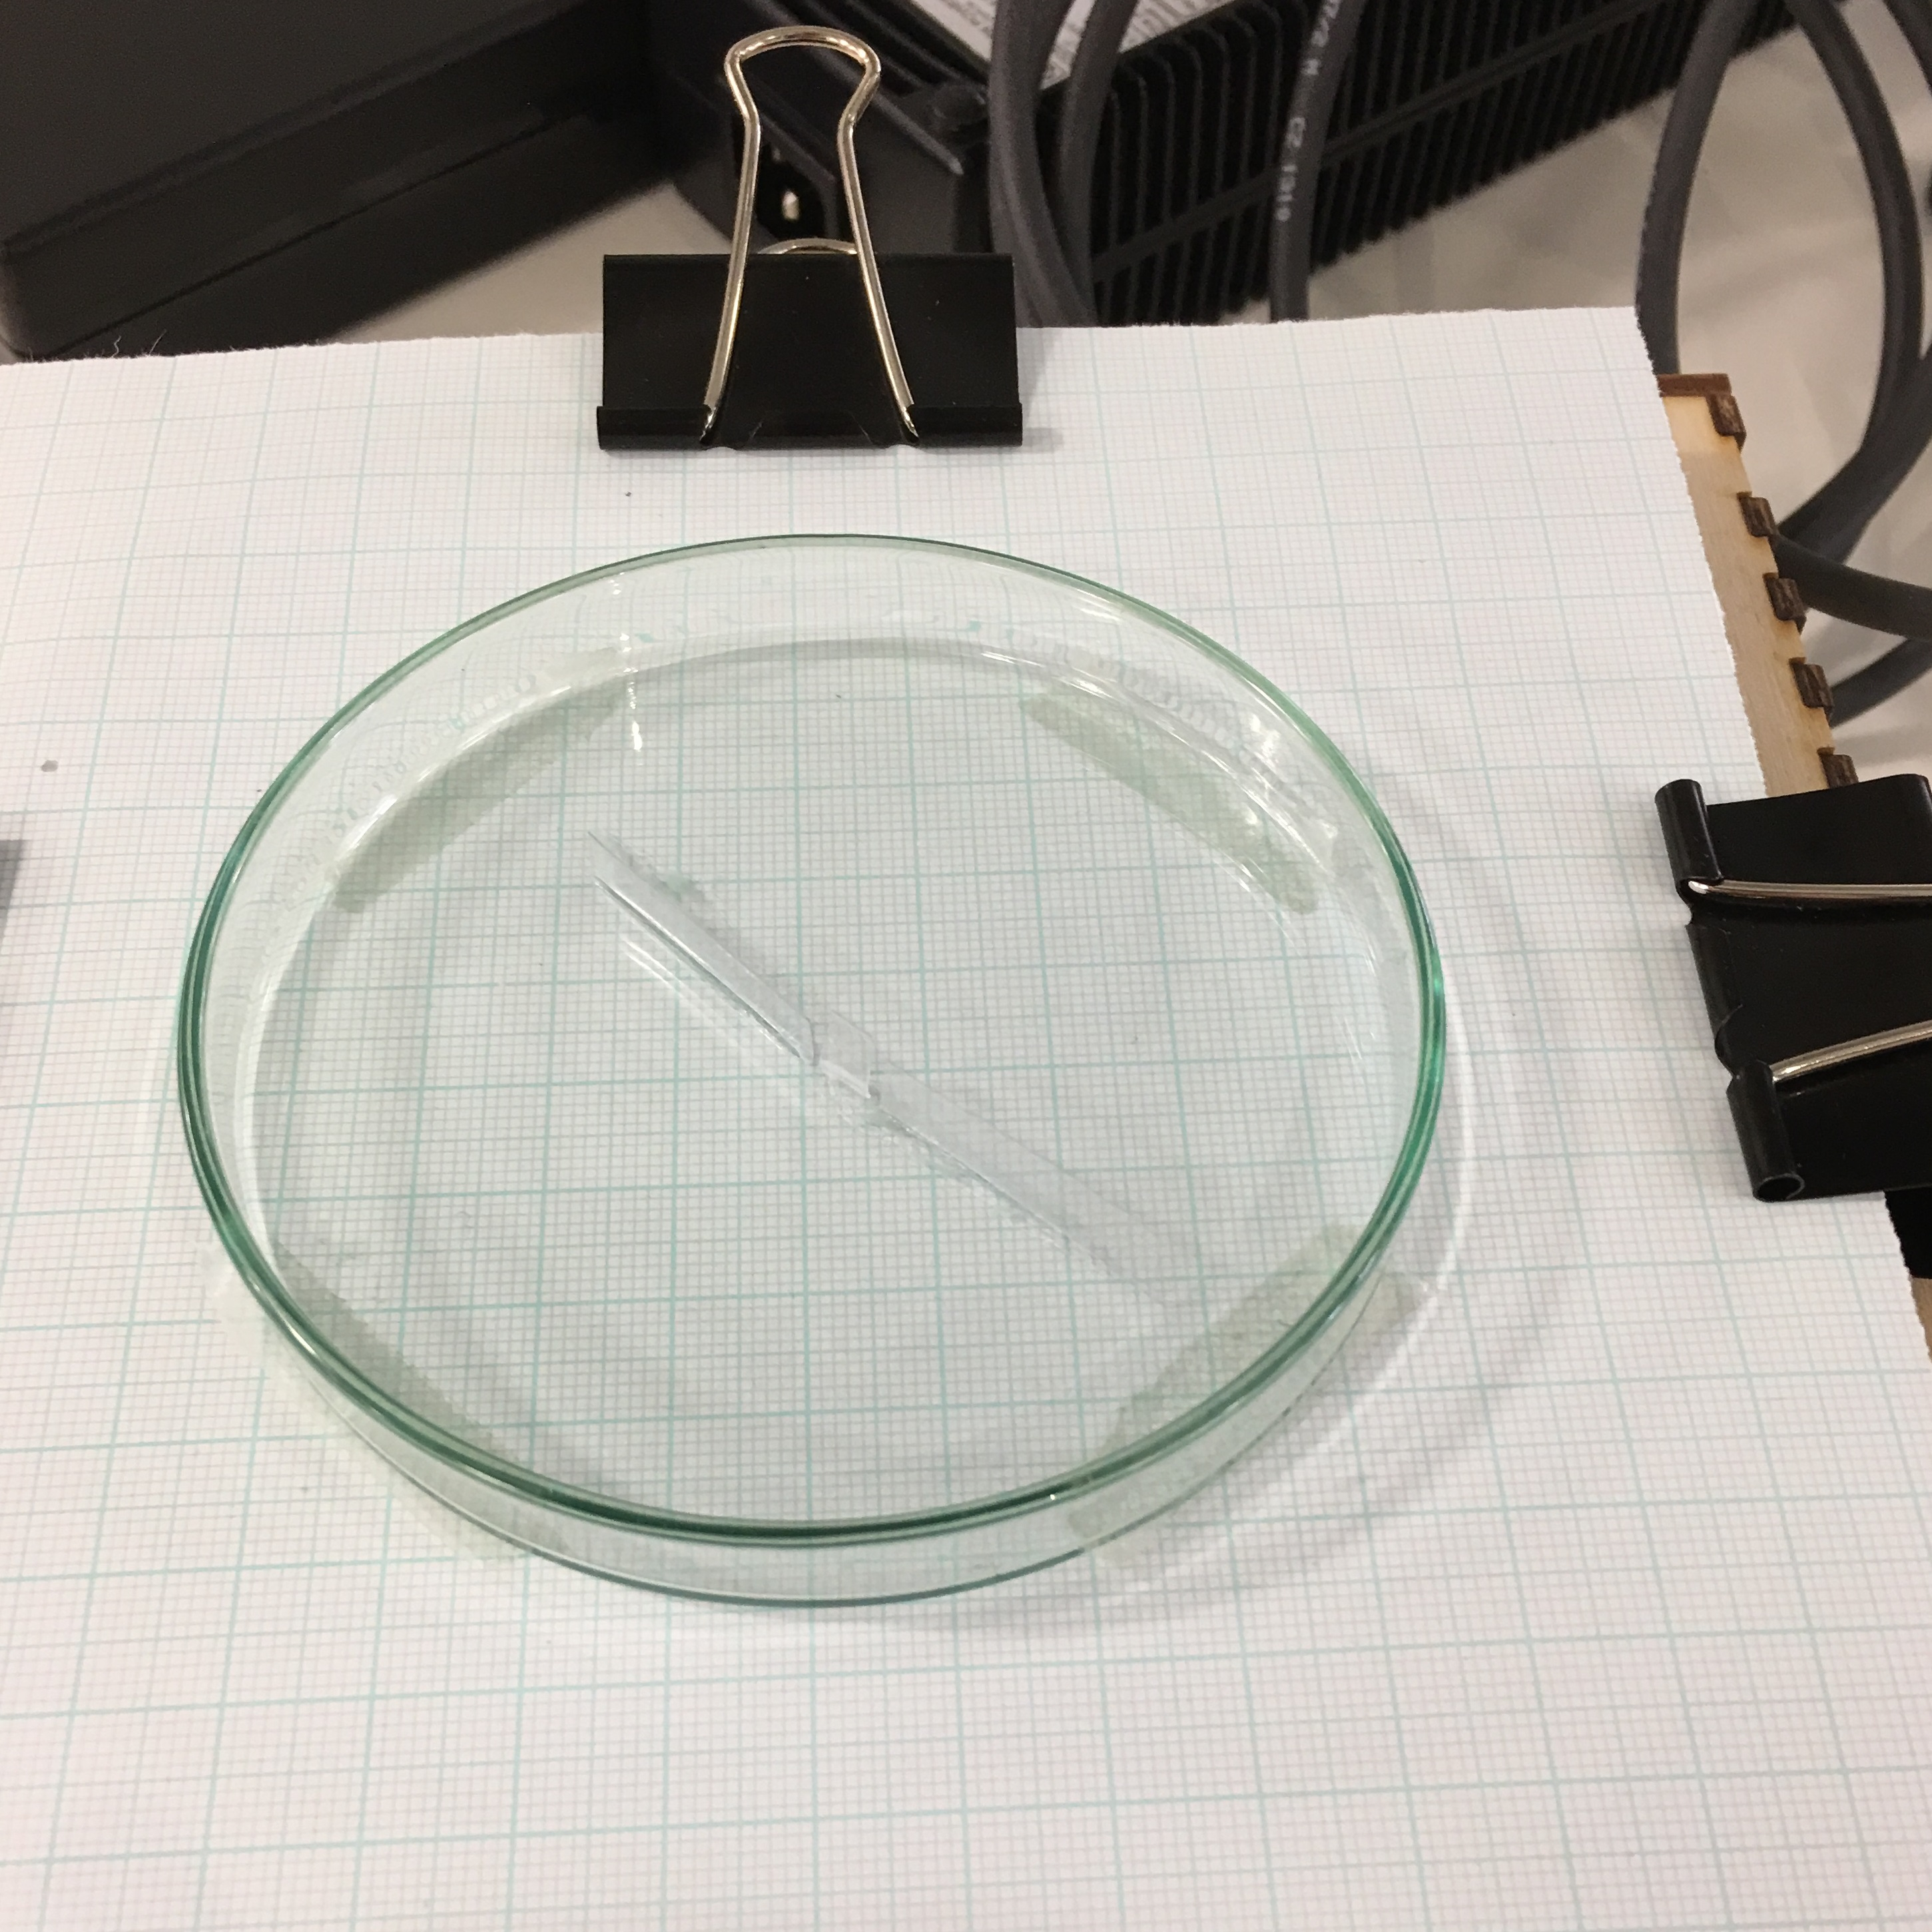
\includegraphics[width=0.5\textwidth]{prototype/exp_rep_imgs/plastic_slits.jpg}
\centering
\caption{Plastic slits were superglued onto the petri dish to form a diffraction grating. This was thought to have a lower surface tension than wood gratings due to the reduced thickness.}
\centering
\label{fig:plastic_slits}
\end{figure}

Initially the frame rate was set to 1000 fps with a resolution of 1024 x1024, giving a video time of around 8 s. A trade-off had to be made between resolution and maximum frame rate, as the highest frame rate at this resolution is 5400 fps. If a higher frame rate was required, the resulting video would have a lower resolution. The trigger was controlled on the computer, and other calibrations were also carried out with the software interface. The setup can be seen in Figures \ref{fig:closeup_highspeedcamera} and \ref{fig:software_highspeedcamera}. The amount of light captured by the lens could also be adjusted, but was usually set to the highest setting, although it was found that lowering this could help with visualisation, since the region was well illuminated due to the presence of the two high-powered lights. In high-speed mode, bouncing and walking were captured. There was difficulty in producing other phenomena, this due to the limited region that was focused on. Sometimes the droplets had to be forced into focus, and this often caused them to break.

\begin{figure}[ht]
    \begin{subfigure}[t]{0.475\textwidth}
        \centering
        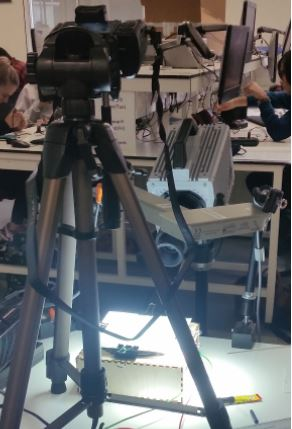
\includegraphics[width=\textwidth]{prototype/exp_rep_imgs/closeup_highspeedcamera.jpg}
        \caption{Closeup on the focusing angle of the high speed camera. Another professional camera was also used to take still images.}
        \label{fig:closeup_highspeedcamera}
    \end{subfigure}
    \begin{subfigure}[t]{0.475\textwidth}
        \centering
        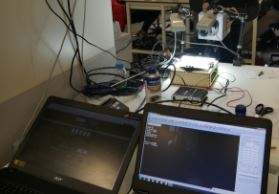
\includegraphics[width=\textwidth]{prototype/exp_rep_imgs/software_highspeedcamera.jpg}
        \caption{Laptops with online function generator and the Photron software, PFV Ver.3681.}
        \label{fig:software_highspeedcamera}
    \end{subfigure}
\caption{Setting up of the high speed camera Photron Fastcam SA1.1, accompanied with high intensity lights and software system}
\label{fig:highspeed_setup}
\end{figure}

Remarkable results were captured with the high speed camera which are summarised and displayed as follows:
\begin{enumerate}
\item  Individual wave fronts were clearly visible, as seen in Figure \ref{fig:highspeed_wave}.
\item  Attempts were made to observe the interference of droplet waves with slit, and to continuously create waves and observe their interaction with  the slits.
\item  Multiple droplets were produced and their interactions with each  other and with the surface are displayed in Figure \ref{fig:highspeed_multiple}.
\item  The Faraday instability regime at high speed is displayed in  Figure \ref{fig:highspeed_faraday}.
\end{enumerate}

\begin{figure}[htb]
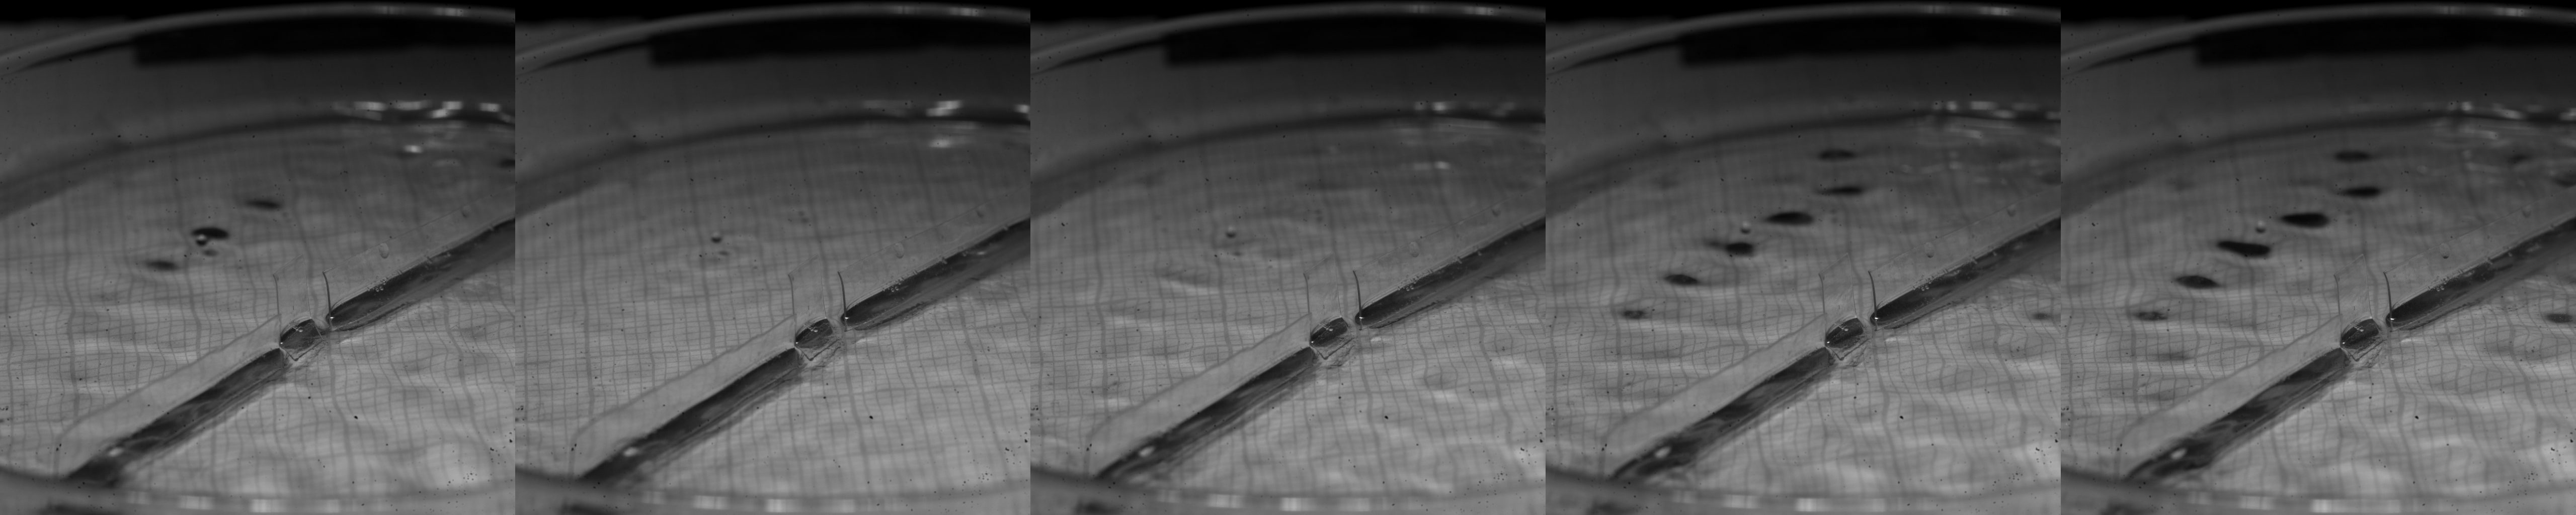
\includegraphics[width=\textwidth]{prototype/exp_rep_imgs/highspeed_wave.jpg}
\centering
\caption{Single droplet standing wave recorded at 1000 fps, series is composed of images taken at every 5 frames.}
\centering
\label{fig:highspeed_wave}
\end{figure}

\begin{figure}[htb]
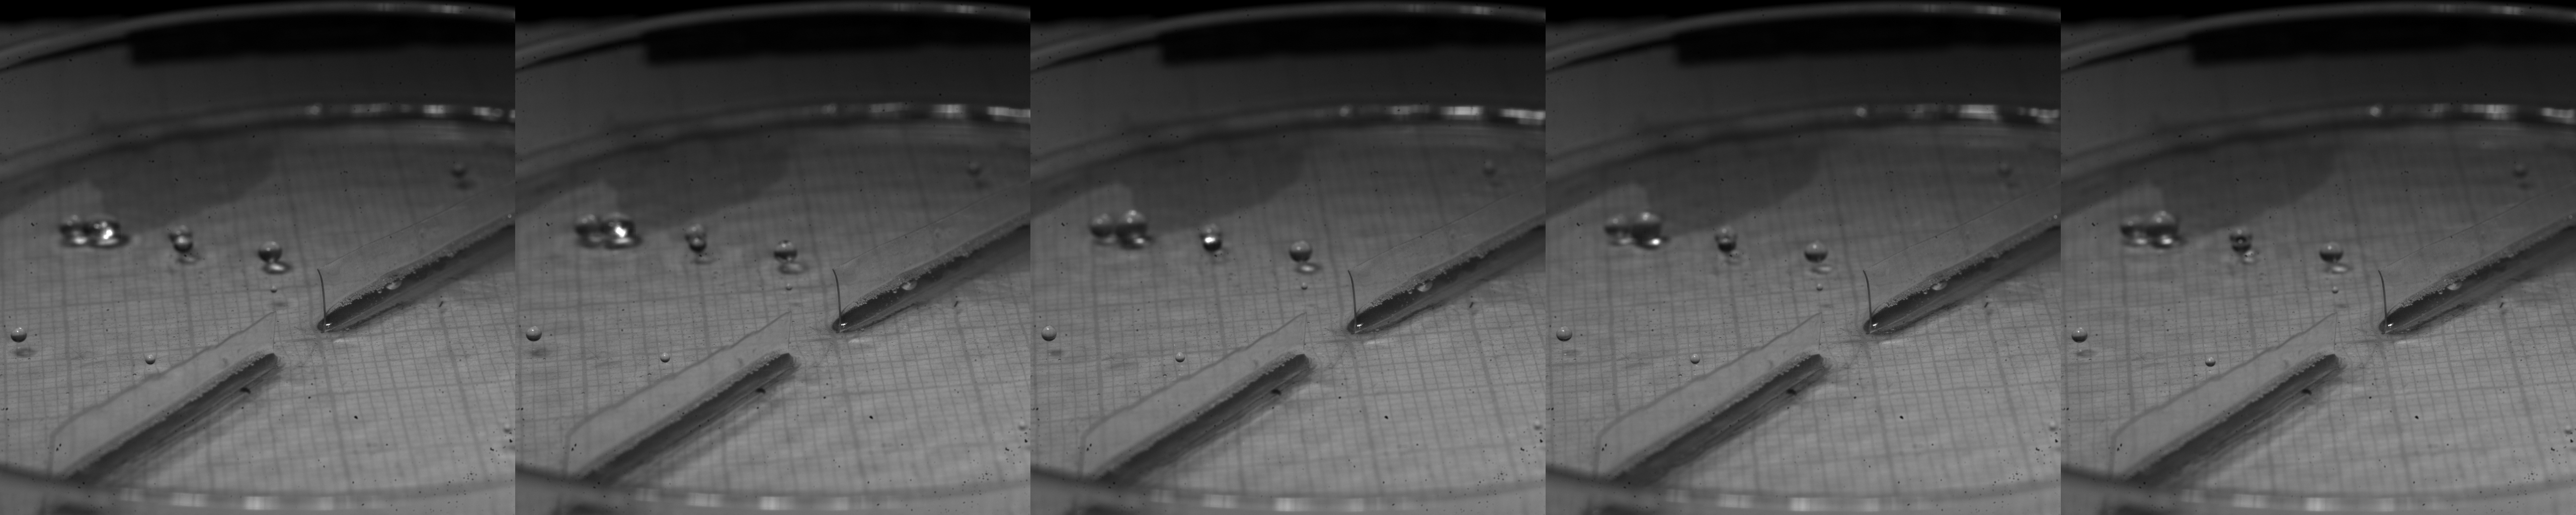
\includegraphics[width=\textwidth]{prototype/exp_rep_imgs/highspeed_multiple.jpg}
\centering
\caption{Multiple droplets displaying standing waves and bound states recorded at 1000 fps, series is composed of images taken at every 5 frames.}
\centering
\label{fig:highspeed_multiple}
\end{figure}

\begin{figure}[htb]
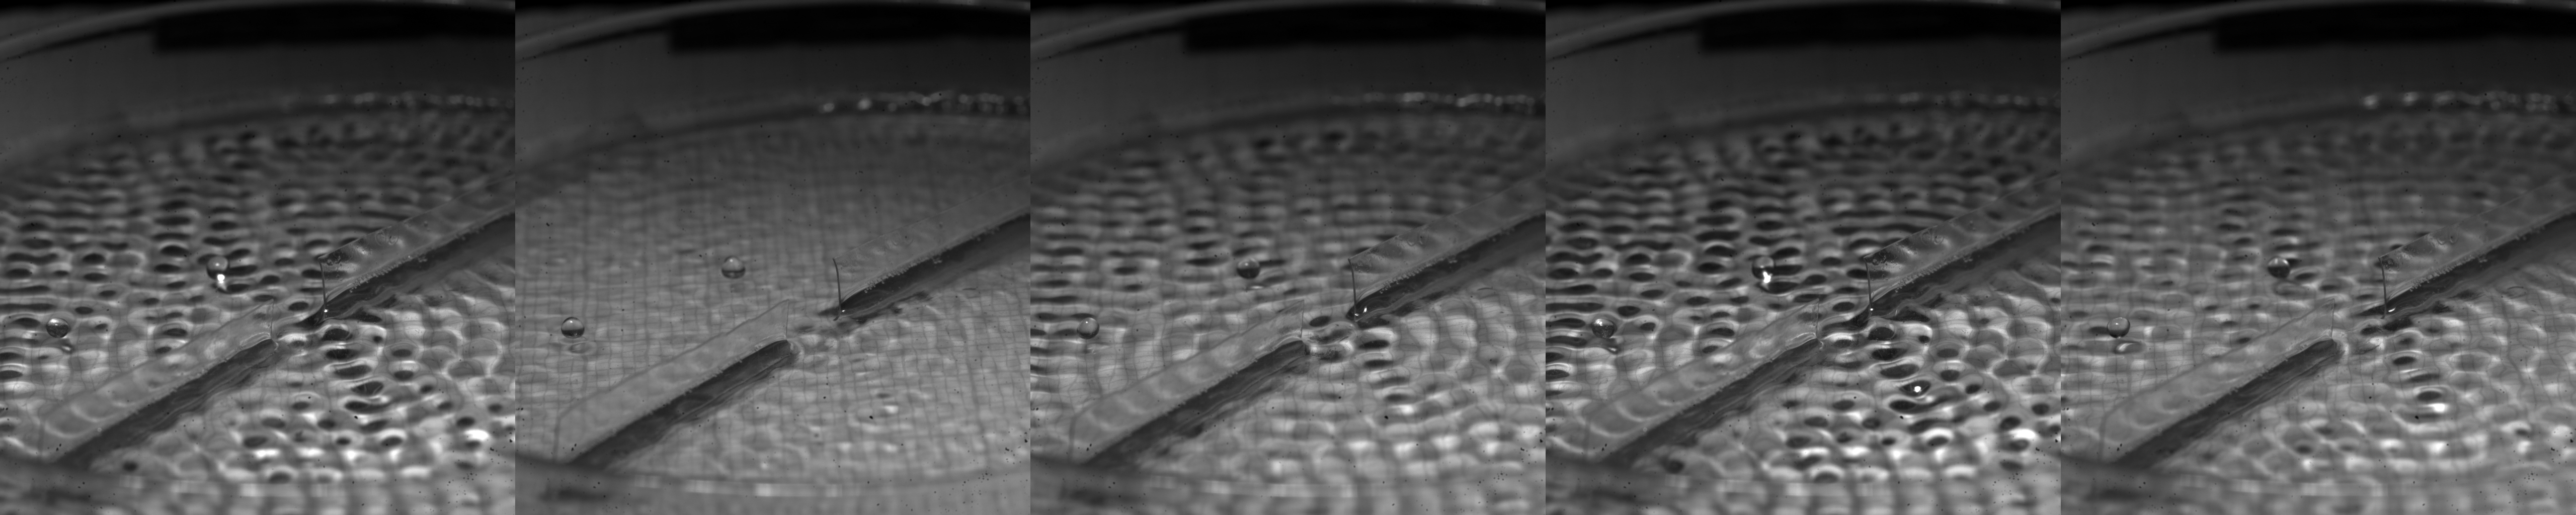
\includegraphics[width=\textwidth]{prototype/exp_rep_imgs/highspeed_faraday.jpg}
\centering
\caption{The surface of the soap water under the Faraday instability regime, recorded at 1000 fps, series is composed of images taken at every 5 frames.}
\centering
\label{fig:highspeed_faraday}
\end{figure}

Motion tracking was postulated to be able to track the high speed footage at a high level of accuracy. This was carried out in Adobe AfterEffects, where the tracking results are illustrated in Figure \ref{fig:tracking_droplet}.

\begin{figure}[htb]
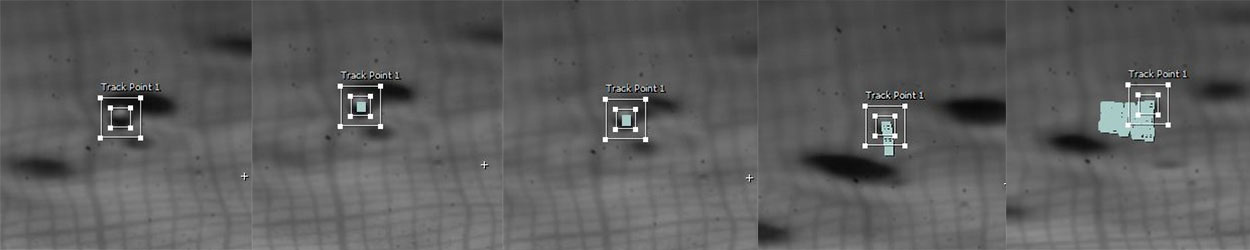
\includegraphics[width=\textwidth]{prototype/exp_rep_imgs/tracking_droplet.jpg}
\centering
\caption{Motion tracking carried out on Adobe AfterEffects, the buildup of white dots represent the path of the droplet in the form of coordinates.}
\centering
\label{fig:tracking_droplet}
\end{figure}

By applying motion analysis to a null object created in AfterEffects,  a sequence of time frames was created as shown in Figure \ref{fig:after_effects_interface}. The time frames were copied into a text document and imported into Microsoft Excel.

\begin{figure}[htb]
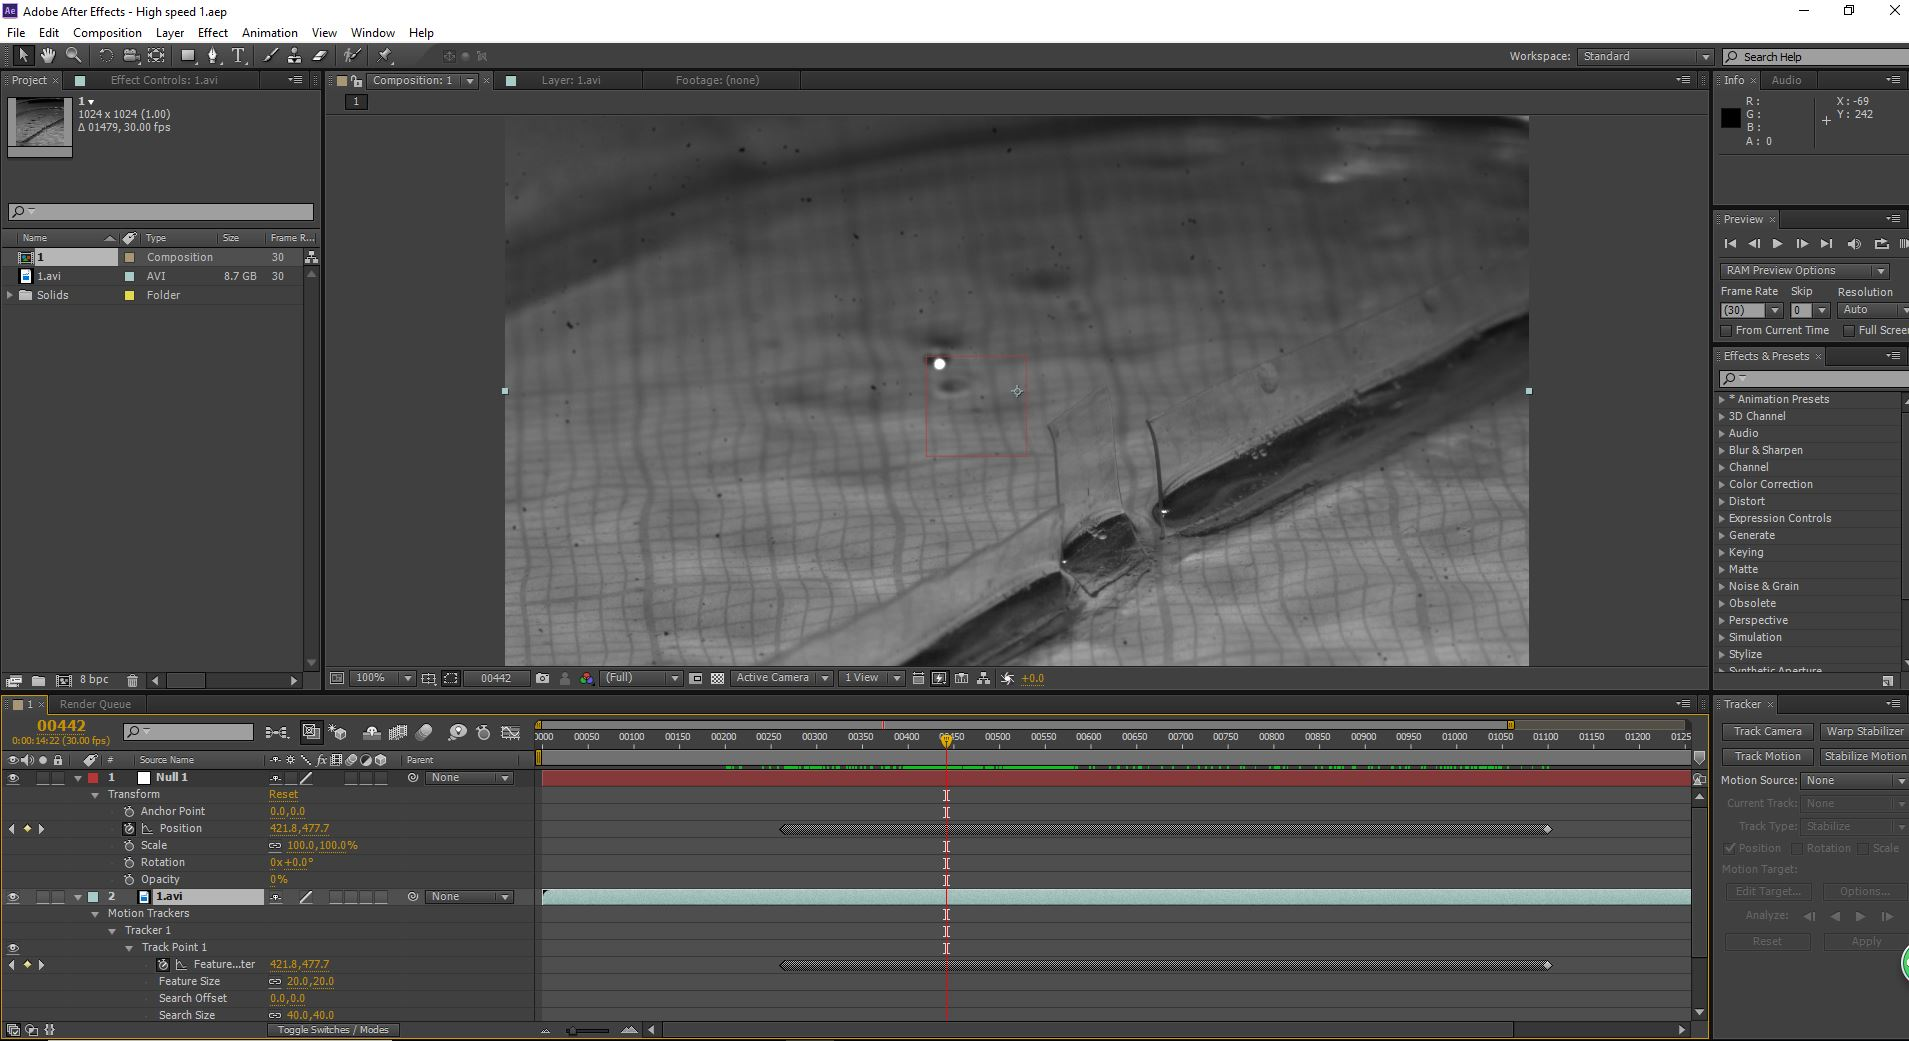
\includegraphics[width=\textwidth]{prototype/exp_rep_imgs/after_effects_interface}
\centering
\caption{A screen-shot of Adobe AfterEffects interface after tracking had been analysed. Key frames are clearly visible on the timeline where they have been applied onto the null object}
\centering
\label{fig:after_effects_interface}
\end{figure}

The exported coordinates were of the format: frame, x coordinates, y coordinates. The coordinates were given in units of pixels. Since the video was recorded at 1000 fps, each frame corresponds to 1 ms. The y coordinates were plotted as a function of time, as shown in Figure \ref{fig:droplet_amplitude_graph}. Converting to time units allowed for a clearer representation of the time scale of bounces.

\begin{figure}[htb]
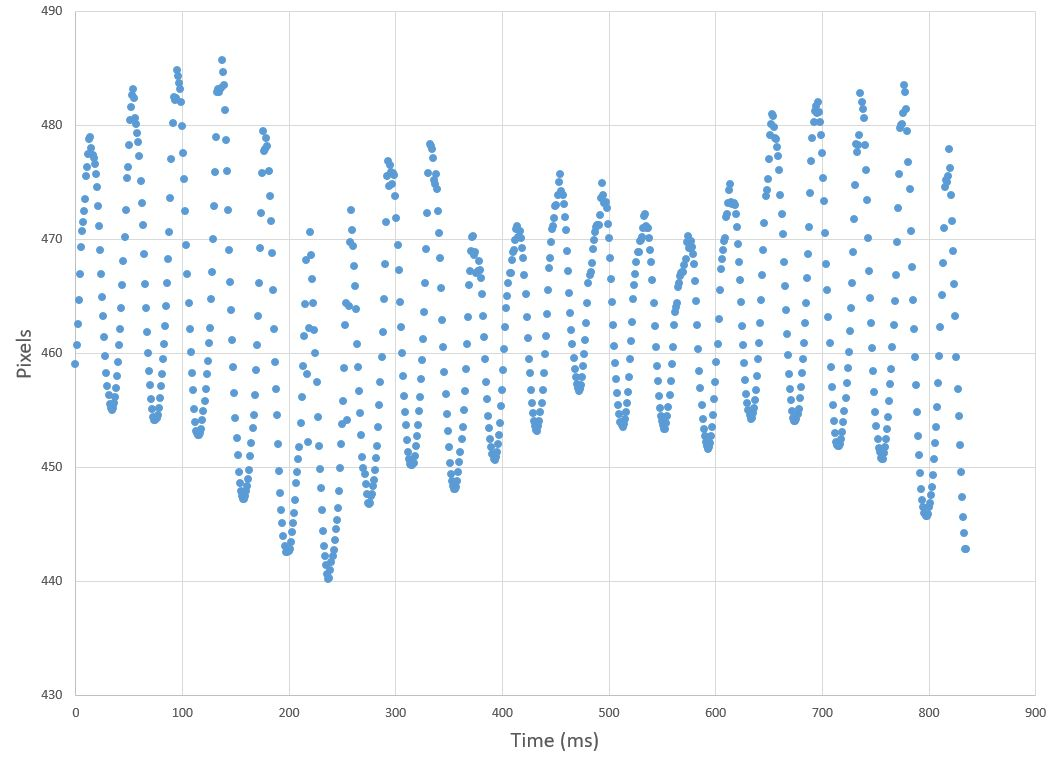
\includegraphics[width=\textwidth]{prototype/exp_rep_imgs/droplet_amplitude_graph.jpg}
\centering
\caption{The y coordinates of the bouncing droplet as a function of time. Oscillatory motion can be seen, and the period is roughly constant.}
\centering
\label{fig:droplet_amplitude_graph}
\end{figure}

Inferences can be drawn from this graph. First of all, the y coordinates do not strictly represent the height of each bounce. This is because the camera is not aligned with the surface of the liquid, but at an angle, due to limitations in focusing and capturing sufficient light. However the main contribution to the y coordinates is the change in height, so the graph clearly demonstrates an oscillatory motion of constant period. Difficulties in determining a quantitative measure of height arose due to the y coordinates being a relative measure. A control needs to be set in order to quantify the y coordinates in units of length. For example, knowing the exact length of an object that is captured by the high speed camera. This allows for a comparison between length and resolution.

A rough estimate of height could be carried out since the diameter of the petri dish was known. The plastic grating is somewhat centred on the diameter of the petri dish. Using Figure \ref{fig:plastic_slits}, the centre of the petri dish can be estimated to be on the right edge of the centre grating. Drawing a straight line upwards to the edge of the petri dish gives an estimate of the radius which is known to be 5.08 cm. The resolution of the video was known, as it was set on the high speed camera to be 1024x1024. The distance to the edge was measured to be about 430 pixels. This means that the length conversion is 0.118 mm per pixel. Typical amplitudes from Fig. 30 are about the size of 15 pixels, which gives a height close to 1.8 mm. This is overestimated as the video was captured at angle of around 30 degrees as seen in Figure \ref{fig:closeup_highspeedcamera}. This stretches out the actual length, and can be compensated for by multiplying by the sine of the angle, which gives around 0.9 mm.  

From Figure \ref{fig:after_effects_interface} it can be seen that there is a bright dot at the bottom of the droplet. This was found during the review of the entire high speed video. During some of the bounces, it seems that a bright beam of light was produced. A frame by frame investigation of this phenomenon was conducted. This can be seen in Figure \ref{fig:strange_light} where a droplet completes a bounce.

\begin{figure}[htb]
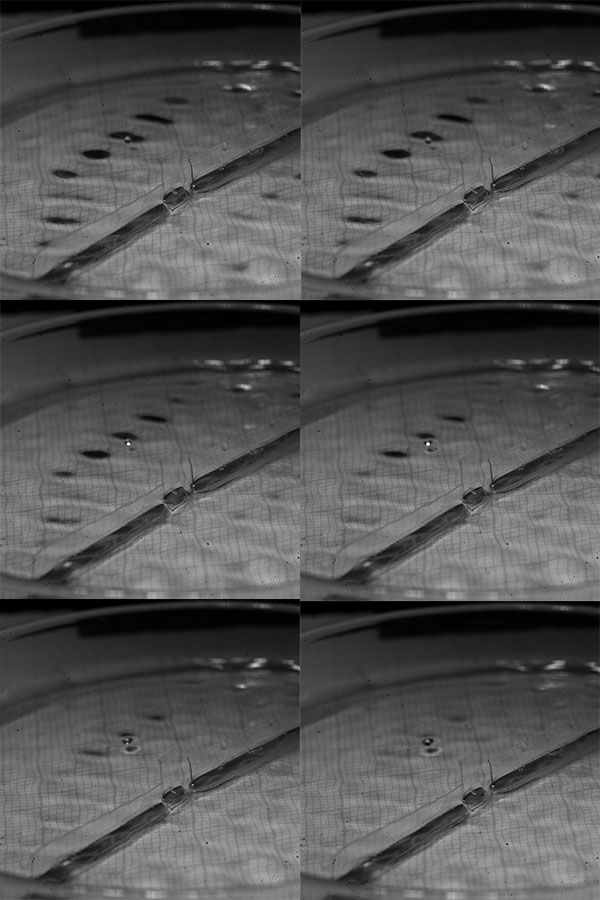
\includegraphics[width=0.8\textwidth]{prototype/exp_rep_imgs/strange_light.jpg}
\centering
\caption{A frame by frame capture of the droplet motion and the formation of standing waves. In the middle two images a white dot can be seen for a few of the bounces.}
\centering
\label{fig:strange_light}
\end{figure}

This was an unexpected result. Close inspection of the high speed video gives interesting qualitative results. Certain bounces are actually two consecutive bounces with the first having a very small amplitude. Bounces that produce a beam of light are single bounces and seemed to propel to a greater amplitude. This suggests some sort of momentum conservation. Light beams also seem to occur from consecutive bounces. The droplet also seems to produce larger wave ripples as it hits the liquid surface. It is hypothesised that at certain oscillations, the droplet has built up enough potential energy to produce more energetic waves and even light. From Fig. 31, it also can be seen that the beam of light existed for longer than 1 ms since this is a frame by frame representation and the video was captured at 1000 fps. This means that it cannot be a single photon. A cascade of photons is required to capture a prolonged period and large cross section, which acts like a laser. There has been research conducted that suggested the possibility of droplets demonstrating atomic electron cloud density under the Faraday regime \cite{oza2013trajectory}.

Further investigation was done in trying to figure out the cause of horizontal motion under the bouncing regime. This was not visible using the naked eye, which is why it remained unknown until now. A possible explanation lies in the use of the plywood plate and foldback clips. There could be random impulses due to the transmission process through the plate. The transmission of waves through a different material is much more complex, and could have resulted in a modified driving force. The sinusoidal waveform could interact with itself in the wood and superimpose to produce another waveform, which can also explain why the amplitude is not constant.

The horizontal impulse is due to the droplet colliding with the side of the bulge, as explained in \ref{theory}. The inclined surface can further complicate the propagation of light. The high intensity light was positioned such that it is almost normal to the surface of the liquid. A portion of it will transmit into the liquid, while others reflect on the surface. The transmitted intensity can further reflect off the bottom of the petri dish or transmit through. The bulge of the wave can act as a medium that focuses light and sends through a coherent beam under certain conditions.

\subsection{Improvements and Considerations}
The table-top demonstration has shown to be effective in producing various droplet behaviours that were predicted by theory. It has fallen short in trying to test diffraction phenomenon or producing more quantitative results, but the progress has been very promising given the time frame and budget. To motivate further investigation, improvements and considerations have been proposed which will be discussed.

\subsubsection{Branding}
The team wants to give the device a distinct branding to show its identity, if it were to be commercialised. Possible considerations include painting the plywood box and printing a ``UCL'' logo. There have been unique and creative methods adopted, such as using foldback clips as clamps or graph paper as a grid. These methods were chosen such that they are extremely reproducible by anyone with a basic knowledge of the setup. This is something that the team wanted to show: a device that is cost-effective, yet very attractive, which is why giving an identity is seen to be very important.

\subsubsection{Improving the plywood box}
In this project, the height of the plywood box was slightly too short, such that plywood finger joints had to be inserted into the gap below the loudspeaker to secure it. One solution will be to laser-cut a new box with the corrected dimensions. However, a more cost-effective method would be to cut circular plywood rings to replace the finger joints, which would fit perfectly in the gap, as the loudspeaker is circular itself. The circular ring would also be more reliable, as it is regularly shaped and provides better support at all angles.

\subsubsection{Rotating liquid bath}
An additional centripetal acceleration would be applied through a rotating bath. The petri dish would therefore experience a vertical force from the loudspeaker, superimposed with a central force that acts towards the centre of the petri dish. This could cause droplets to be forced toward the centre.

Depending on the speed of the rotation, it may not cause the droplets to move in the direction of the centripetal acceleration. There is always a degree of restoring force due to surface tension which has to be overcome. This provides a measure of restoring force since the centripetal force can be calculated using \ref{equ:centripetal_force}:
\begin{equation}
F_c = \frac{mv^2}{r} = m \omega^2 r 
\label{equ:centripetal_force}
\end{equation}

For two droplets that are 'repelling' this will create the illusion that they are orbiting each other

\subsubsection{Observing a double slit interference pattern}
This experiment has demonstrated, enough phenomena (`bouncing', `walking', `orbiting', surpassing of Faraday regime etc.) to provide evidence for the Pilot-Wave theory, which opposes the Copenhagen interpretation of quantum mechanics. With this, double slit interference should be observable provided that enough droplets travel through the slits and their end position is recorded. It was thought that a high speed camera should be able to capture the wave's interaction at the slit, and how two waves interfere with one another at close range.

\subsubsection{Observing quantum tunnelling}
Quantum tunnelling was observed by another research group \cite{brady2014bouncing} whereby there is a barrier at the edge of the petri dish, and a body of fluid on the other side also driven at the same frequency. It was shown that on rare occasions the droplet was able to pass through the finite width barrier and end up on the other side. This result proves the possibility of observing quantum tunnelling, a purely quantum phenomenon, at a macroscopic scale.

\subsubsection{Improvements on motion tracking}
It has been demonstrated that the droplets follow irregular motion within the Faraday regime. By recording the droplet motion for a prolonged period of time, it could be shown that the resultant path has high levels of similarities to the atomic electron cloud density. 

This is likely to be feasible with the current setup and software. A proper top-down video needs to be captured in order to eliminate parallax and scaling errors. The difficulty would lie in the tracking process, as the chaotic surface hinders the tracker's ability to follow the droplet. However, the video can be broken down into shorter pieces, where each piece is tracked individually. By reconstructing the entire path through plotting the time frame coordinates, a similar pattern should be found.

\subsubsection{Method of producing droplets}
A common issue faced was producing droplets of consistent size. Multiple mechanisms were thought of, including a spring loaded pinpoint which would oscillate vertically and constantly dip into the fluid and create a droplet.

Another proposal was for a rotating mechanism which has multiple pinpoints of constant separation on a wheel. Once rotated, each pinpoint would prick the surface and create a droplet. This has the benefit of producing multiple droplets very rapidly and of providing them with horizontal momentum, which could be used to push droplets towards any desired direction. This may be beneficial in testing double slit interference, where droplets need to travel through thin slits.



\clearpage
\section{Simulation (JAL, CKG, GA, AS)}
The simulation team aimed to construct an interactive software package that could simulate and visualise the motion of droplets bouncing on a liquid surface. The goal here was to cover aspects of quantum mechanics that would not be displayed by the prototype, such as double slit diffraction and tunnelling effects.
\subsection{Initial work in python}
Initially, work undertaken by the simulation group consisted of finding suitable mechanical descriptions of the droplet's motion, and implementing those in code. A simplified model was taken from \cite{brady2014bouncing}, where the droplet was treated as stationary in the x-y plane and moving in z according to (\ref{equ:basicHeight}). Here, $h_0$ is the maximum height of the drop, $\omega_0$ is the driving frequency of the system, r is the displacement of the drop from the centre in polar co-ordinates and c is the speed of the wave. $J_0$ is a Bessel function of the first kind. With $\omega_0$, r and c set arbitrarily to 1, wave motion was demonstrated using an animation framework from \cite{waveanimation}. The results of this are shown in Figure \ref{fig:basicAnimation}. Unfortunately, the python language used to generate this proved too slow to be usable as a live demonstration, so any simulations generated using this method would need to be exported to a movie file and played back later. Initially, this was deemed an unacceptable solution, and so Java was chosen as a more efficient language to use in future.

\begin{equation}
    h = -h_0 \cos{(\omega_0 t)} J_0 (\omega_0 r/c)
    \label{equ:basicHeight}
\end{equation}

\begin{figure}[h]
    \begin{subfigure}{0.5\textwidth}
        \centering
        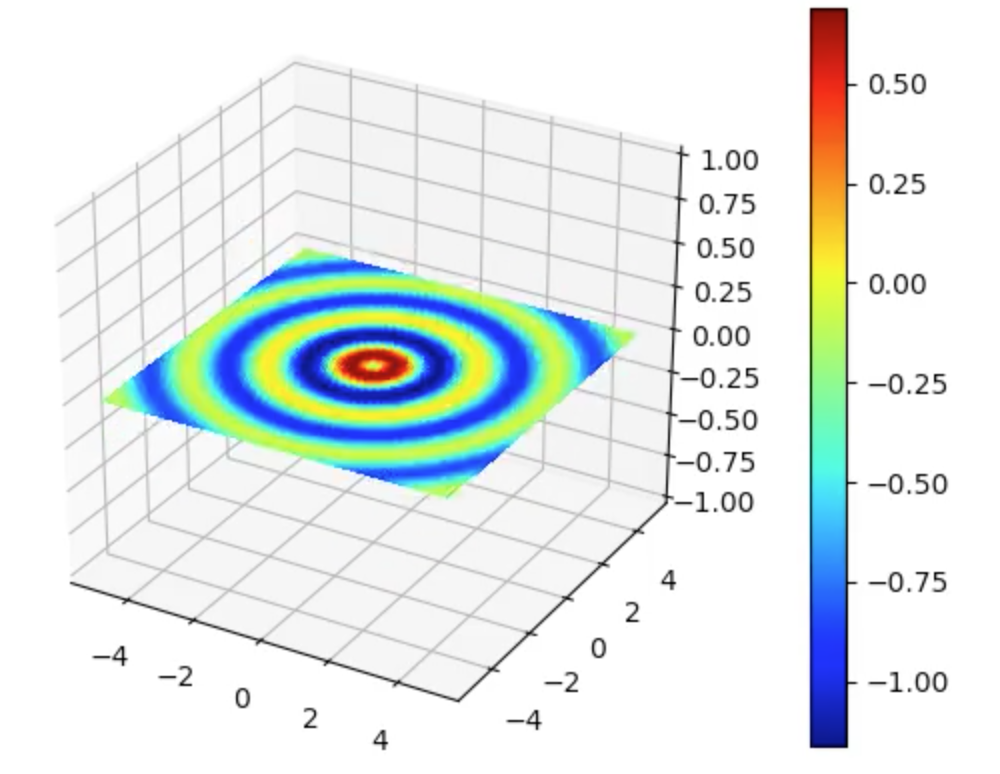
\includegraphics[width=\linewidth]{simulation/basich0.png}
        \caption{Wave motion at $h=0$}
    \end{subfigure}
    \begin{subfigure}{0.5\textwidth}
        \centering
        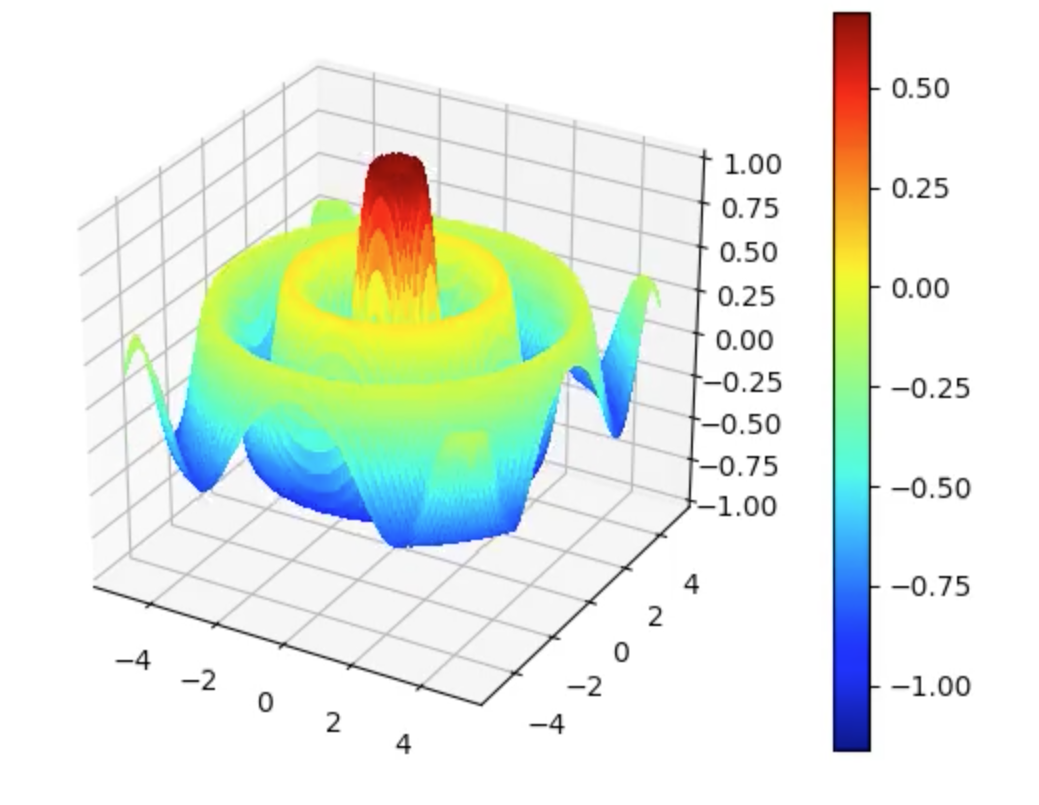
\includegraphics[width=\linewidth]{simulation/basichmax.png}
        \caption{Wave motion at $h=h_0$}
    \end{subfigure}
\caption{Simulation output generated with python and Matplotlib. (a) represents the initial state of the wavefield, while (b) represents the state of the wave-field when the "droplet" at the centre is at its maximum height}
\label{fig:basicAnimation}
\end{figure}


\subsection{Constructing a GUI in Java}
Initially, a Java simulation was developed, which aimed to construct a pixel grid which could be used to represent a wave-field. Objects representing a given data point and a "frame" of these data points were constructed, and populated with amplitudes using (\ref{equ:basicHeight}). These amplitudes were then displayed in 2D by assigning them to an opacity scale, with 100\% opacity representing the maximum possible height and 100\% transparency representing the minimum possible height. For a 40,000 pixel frame running over 10 seconds, this process took approximately 9 seconds, but the animation process after this ran in real time. Figure \ref{fig:javaBasicHeight} shows a still image of this GUI taken when the "droplet" was at a minimum height of $-h_0$. This animation was a success, but at higher resolutions, latency when drawing the pixels to the screen caused it to lag, suggesting a need to either run multiple drawing tasks in parallel, or to display the droplet motion in an alternative way.

\begin{figure}
    \centering
    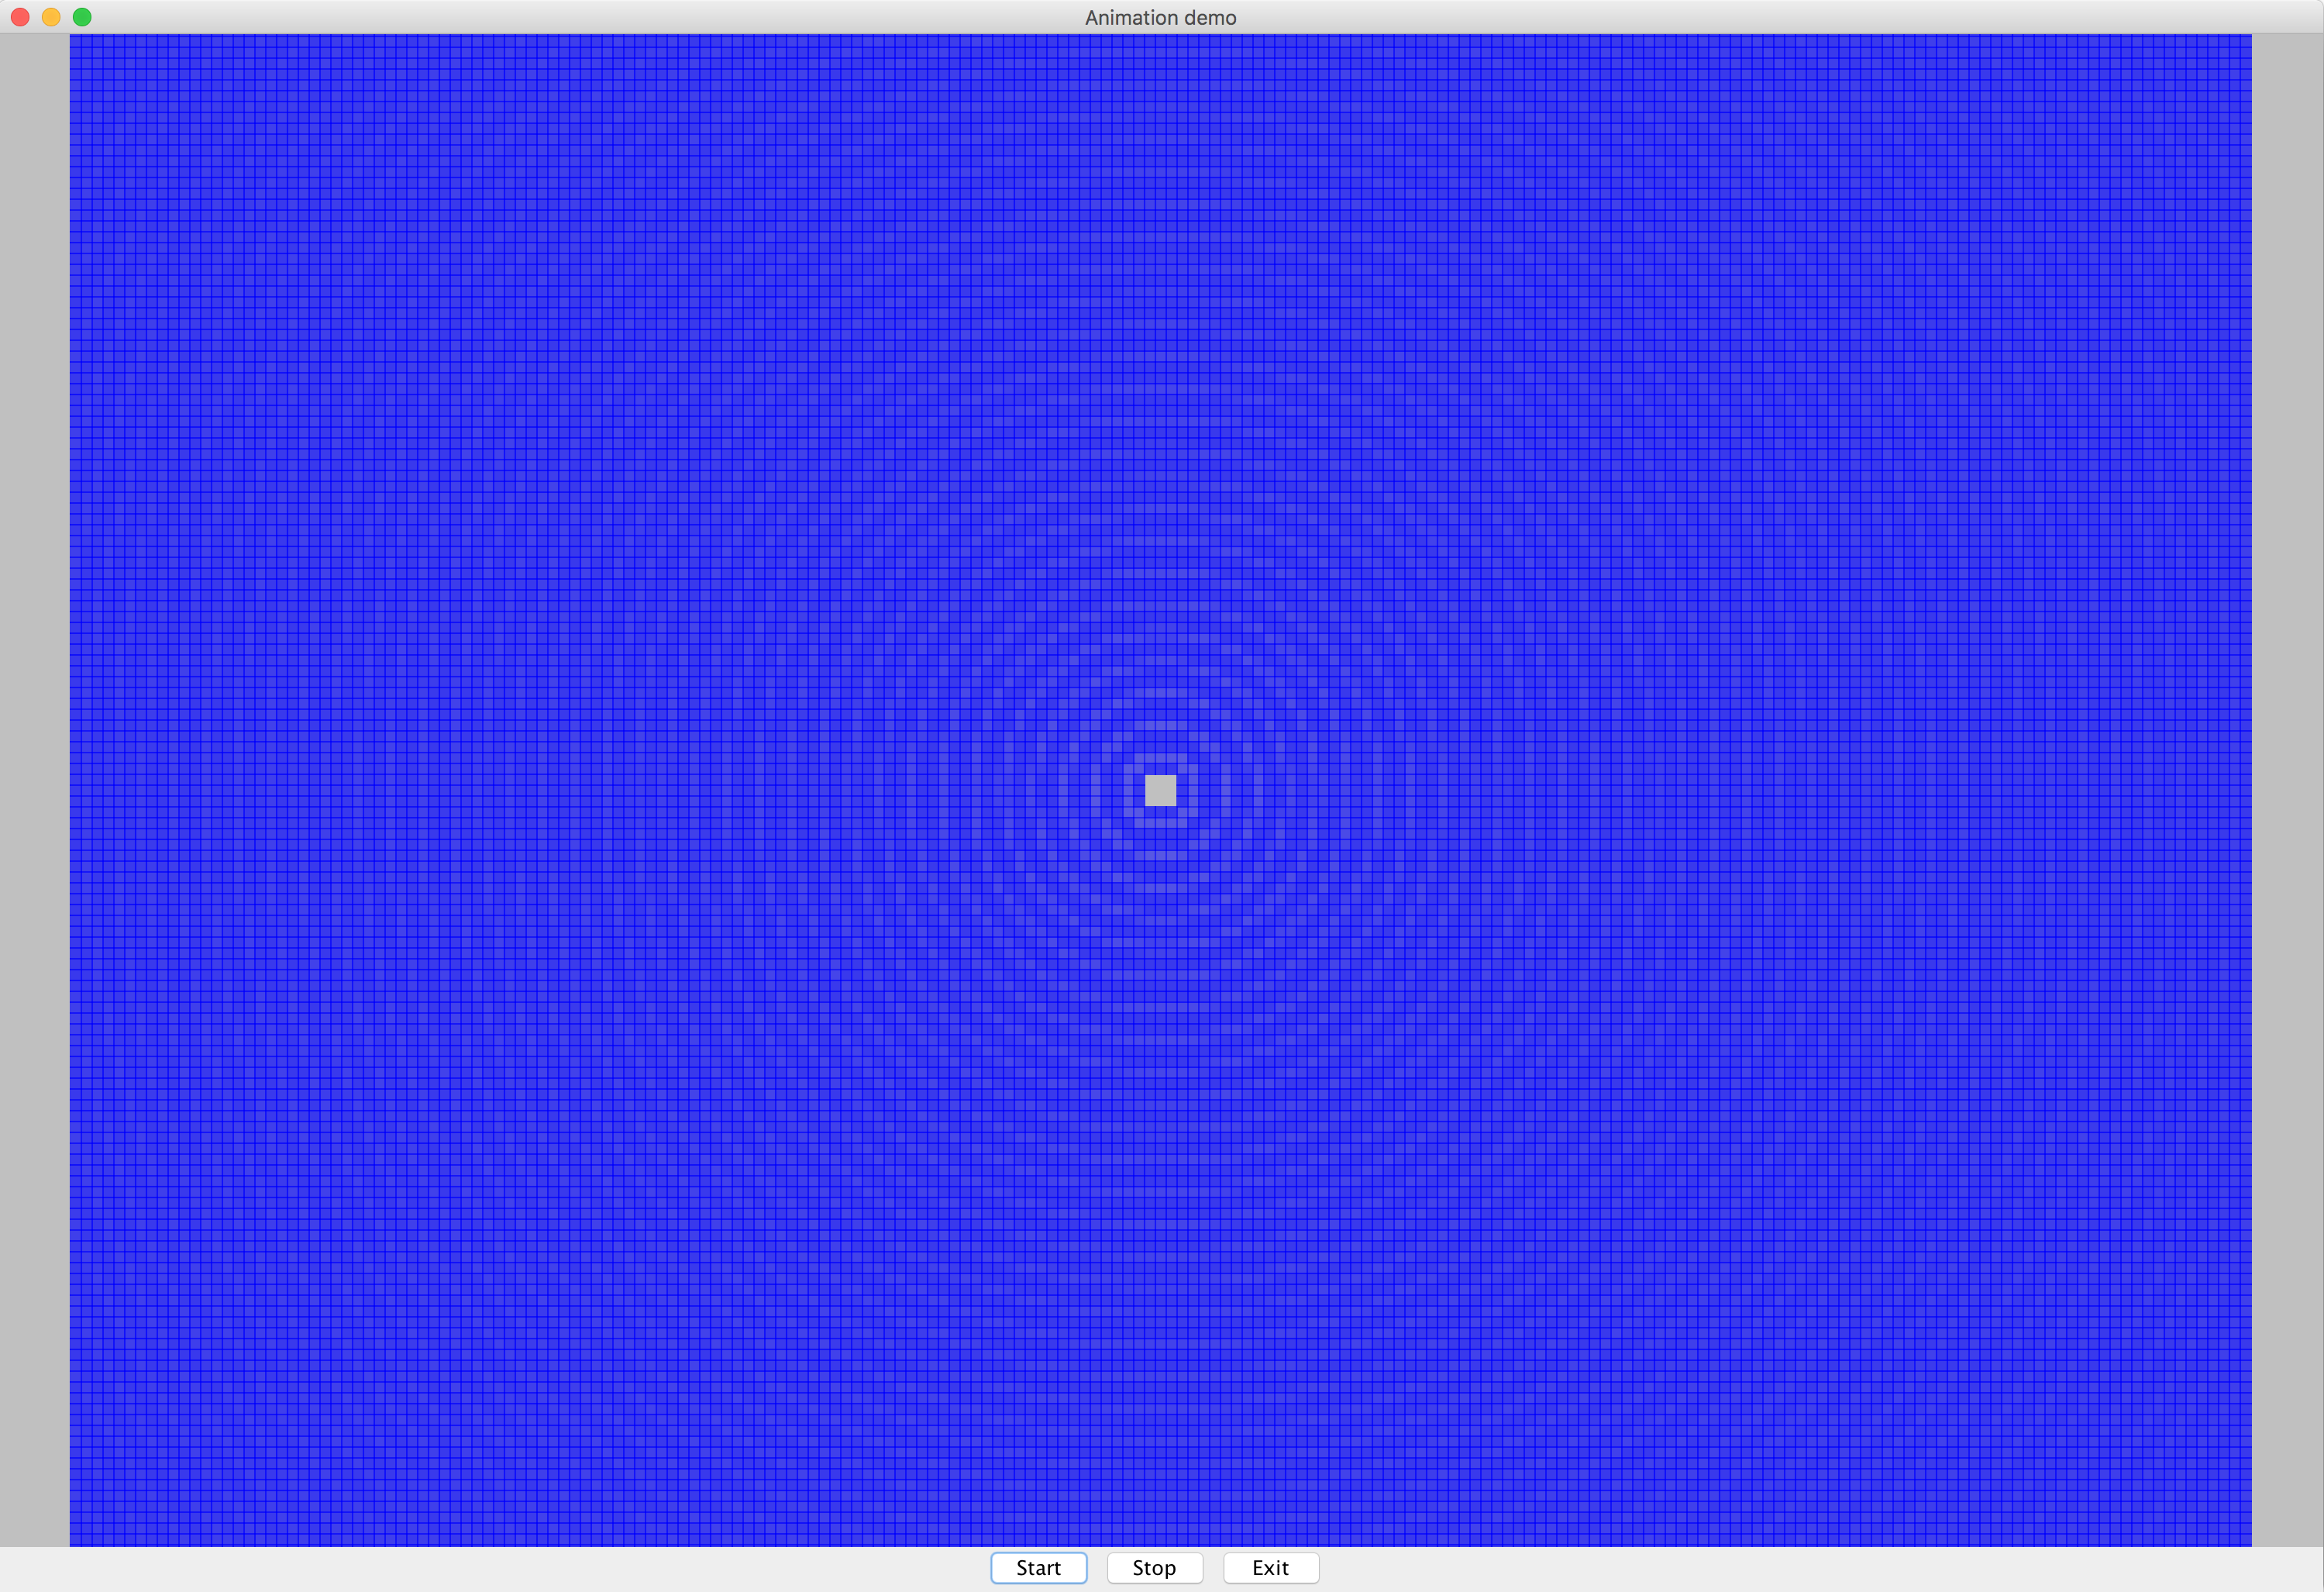
\includegraphics[width=\textwidth]{simulation/javaMaxHeight.png}
    \caption{A basic Java GUI, here showing the droplet at its minimum height of $-h_0$}
    \label{fig:javaBasicHeight}
\end{figure}

\subsection{Probabilistic prediction of position}
Having demonstrated the possibility of displaying wavefunctions in Java, displaying an object representing a droplet was the next task. Here, the assumption was that the wave (described by (\ref{equ:probWaveEqn})) represented a probability density function. Therefore, for a given (and ideally infinitesimal) pixel n of area dA, the probability $P_n$ of finding the particle at pixel $n$ was calculated from that function. The height ($z_n$) of each pixel within that section was calculated, with ${P_n}/{z_n}$ representing the probability of the particle being at that pixel. The sum of probabilities for this section, $Z=\sum_n{P_n}$, defined the normalisation value of the thread. A random number generator then generated a number R such that $0\leq R \leq 1$, which was multiplied by $Z$ to give a relative random number. The program then looped back over all the pixels in the section, and repeatedly subtracts $P_n$ from $RZ$ until $RZ<0$. The first pixel where this condition is satisfied is determined to be the location of the droplet. This process could then be multi-threaded to improve computational efficiency.

The application of this to our project was that once the droplet is found at a given pixel, the distance between that pixel and the next pixel representing the location of the droplet is used to calculate the velocity $v$ of the particle, assuming the droplet moves to the new pixel in the space of one period $T=1/f$. The wavefunction was updated with the new velocity, once a Lorentz transform was accounted for. This whole process is repeated to find the trajectory of the pixel.

\begin{figure}
\centering
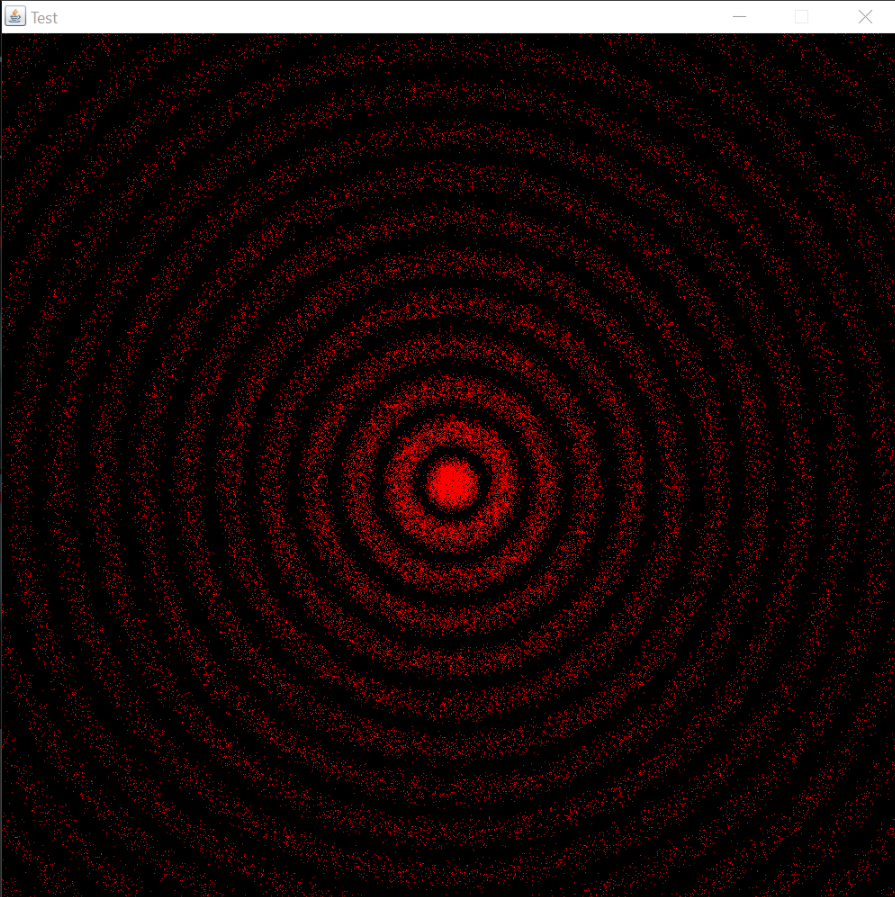
\includegraphics[width=\textwidth]{simulation/probabiltyPosition.png}
\caption{Results of the probabilistic prediction of the droplet position, where each dot represents the droplet being present at this point}
\label{fig:probabilisticPrediction}
\end{figure}

\begin{equation}
    h = -\cos(\omega t) J_0(\frac{\omega}{c} |\vec{r_f}-\vec{r_i}|)
    \label{equ:probWaveEqn}
\end{equation}

Although this process was successful, all it ended up proving was that a random position generator works. It does not accurately simulate the position of droplets created in our experiment. Therefore, we proceeded to calculate the equations of motion and the wavefunction of the droplet at each point.

\todo{Finalise writeup of MATLAB work}
\subsection{Rapid prototyping in MATLAB}
In parallel to this, MATLAB was chosen to test implementations of mathematical concepts found in our research, as it has a wide variety of built in libraries, such as for graphing software and advanced mathematical processes. Initially, equations of motion for the droplet were taken from \cite{oza2013trajectory}, where (\ref{equ:MATLABPilotWave}) defines the wave-field of the particle and (\ref{equ:MATLABWaveHeight}) defines the bath height over time. To implement these, a grid object was constructed and populated with x-y coordinates. A point in the middle of the grid was then selected as the starting position for a droplet, which was used as the centre of modelling for the first interaction.

\begin{equation}
m \vec{x}'' + D\vec{x}' + k\vec{x} = -mg\nabla h(\vec{x},t)
\label{equ:MATLABPilotWave})
\end{equation}

\begin{equation}
h(\mathbf{x},t) = \sum_{n=-\infty}^{\floor{t/T_F}} A \mathbf{J}_0(k_F |\mathbf{x}-\mathbf{x}_p(nT_F)|) e^{-(t-nT_F)/(T_F Me)}
\label{equ:MATLABWaveHeight}
\end{equation}

Once a centre had been chosen, the wave-field generated by the droplet at that point was calculated at time $t=0$. Assuming that the droplet bounces in phase with the forcing frequency, the droplet next interacts with the bath at time $t=T_F$, where $T_F = 2/\omega$, with $\omega$ representing the forcing frequency of oscillation. The evolution of the wave-field during this time period was calculated from the Bessel function $\mathbf{J}_0$, and so the droplet experiences a quasi-instantaneous acceleration proportional to the gradient of the wave-field at the droplet's position. A wave-field is generated at the droplet's new position following this acceleration. This process is repeated, with the $N$ most recent wave-fields added to the current wave-field, where $N$ represents the number of recent impacts used to calculate the wave-field. Each iteration of this process was represented with a frame in the animation, which contained a colour-coded $(x,y,z,t)$ point for the entire grid, as shown in Figure \ref{fig:MATLABMaths}.
\begin{figure}
\centering
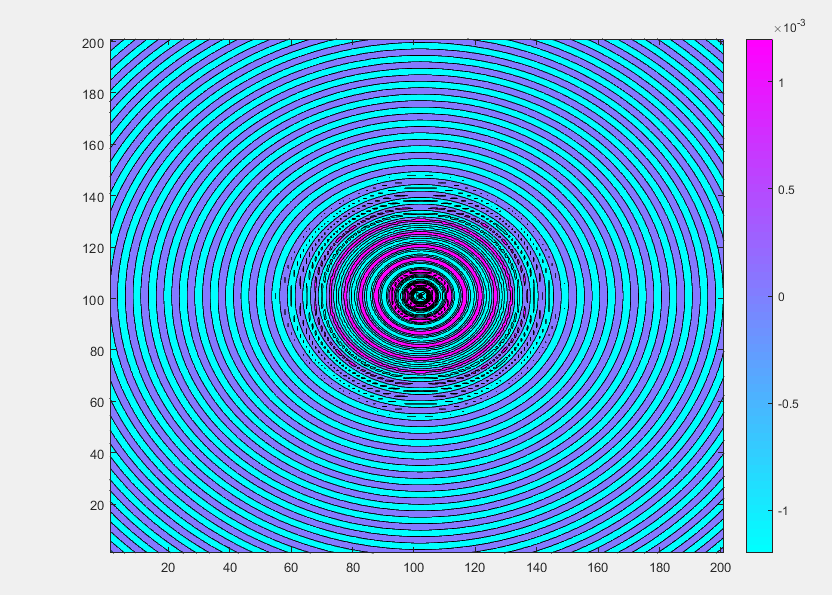
\includegraphics[width=\textwidth]{simulation/matlab.png}
\caption{The wave-field of a single droplet after multiple iterations, with a box size of 200x200 pixels and $N$=16. $N$ was chosen as the machine used was capable of 8 threads and each impact is calculated in parallel}
\label{fig:MATLABMaths}
\end{figure}

\subsection{Modelling assumptions and simulation mechanics}

The following assumptions were made during the simulation: 

\begin{enumerate}
\item The particle and surface waves produced are oscillating in phase with each other.
\item The particle and surface only interact within a small time frame $T_i$, after the particles' lowest point.
\item The average force exerted by the particle over $T_i$ is given by an effective wave force $F_b$. $F_b$ depends on material parameters and the mass of the particle, and tt has a maximum magnitude equal to the weight of the particle.
\item The effect of the Lorentz transform is negligible.
\item The impulse applied to the particle in the vertical direction perpendicular to the surface is assumed to be negligible and the particle continues oscillating vertically at the same frequency and amplitude. 
\item The particle experiences no damping force
\item The overall wave equation $h(\vec{r} , t)$ is dominated by the waves from the last $N$ bounces only. Waves formed longer than $N$ bounces ago are removed from the overall wave equation. This simplifies the computation of the infinite sum within the overall wave equation. In the Java simulation, by integrating multi-threading methods into our calculation, we were able to efficiently perform calculations with $N = 300$.
\end{enumerate}

Following these modelling assumptions, the parameters of the system were set as follows \cite{dotwave}:

\begin{itemize}
\item Particle mass, $m_p = 2.6\times10^{-7}$ kg
\item Driving Frequency $\omega= 80$ Hz
\item Period of particle, $T_f = \frac{2}{\omega}$ s
\item Gravitational acceleration, $g = -9.81$ m/s
\item Effective force, $F_b = 1.3174\times10^{-6}$ N
\item Wave number, $k = 1250$
\item Amplitude, A = $\frac{F_b}{m_pkg}$ m
\item N = 300
\end{itemize}


From the assumptions made above, it can be shown that the change in velocity of the particle in the direction parallel to the surface is given by:
\begin{equation} \Delta \vec{v} = \frac{T_i  F_b}{m_p} \times \frac{dh(\vec{x} , t)}{d\vec{x}}\end{equation}
Where $m_p$ is the mass of the particle and the last term is the vector gradient of the wave.


It was difficult to strike a balance between an acceptable data generation time and simulation accuracy. With simulation values used in the image above, each frame takes over 10 minutes to generate. The largest factor in the total processing time is the number $N$ of previous impacts stored. In the physical situation, the decay of each wave generated at an impact would be dependent only on the $Me$ parameter. \cite{couder11} In numerical simulation, only a limited number of recent impacts can be stored within the memory but ideally the value of $N$ should be chosen such that the contribution of an impact is nearly negligible when it is removed from memory. However, due to computational limitations, only the 16 most recent impacts were used in the calculation of the wave-field. This also precludes the simulation of multiple droplets, as each droplet would result in an additional $N$ impacts being stored.

The issues encountered in terms of processing speed could be partially addressed by porting the mathematical model developed into Java.  While it was expected that this would enable more efficient data generation, the realistic improvement in speed that could be offered would not be able to entirely negate these problems.
It was clear at this point that, regardless of potential optimisation, the goal of having a interactive simulation was not within the scope of the project. It was subsequently  decided to focus on using the previously developed Java graphics system with the aforementioned prototype  to create a number of pre-rendered videos.

\subsection{Integrating Java and MATLAB}

Due to calculation and graphical issues in  MATLAB and Java respectively, a possible solution was the execution of Java classes from a MATLAB script. This would allow the calculations to be carried out in Java, outputted to a csv or text file, and then read by the initial MATLAB script for demonstration. This was implemented using the command() function in MATLAB to navigate to the source folder, compile and then run the necessary classes. Due to time constraints, it was not possible to complete this. The main issue encountered was the use of external .jar files (to implement the Bessel function) not allowing the java files to compile. Various unsuccessful solutions were attempted,so it was decided to move on.



subsection{Java}

Importing the above model from MATLAB into Java was decided as the best course of action. The equations used and assumptions made were identical, but there was a slight difference in the manner which the gradient was calculated.

As opposed to using a built in function, in 1-D, the gradient at a point $x = x_0$ is given by:
\begin{equation} \frac{dy}{dx}\Bigr|_{x_0} = \lim_{x\to0} \frac{y(x+\delta x)-y(x-\delta x)}{2\delta x}\end{equation}

Using a Taylor expansion about $x_0$, it can be shown that for $\delta x\neq 0$:
\begin{equation} \frac{dy}{dx}\Bigr|_{x_0} = \frac{y(x+\delta x) - y(x-\delta x)}{2\delta x} - O(\delta x)\end{equation}
Where $O(\delta x)$ is the residual given by:
\begin{equation}O(\delta x) = \sum_{n=2}^{\infty} \left( \frac{y^{(n)}(x_0)}{n!\times (2\delta x)} \left[ \left( x+\delta x -x_0 \right)^n - \left(x-\delta x -x_0 \right)^n \right] \right)\end{equation}

The 2-D vector gradient of $h(\vec{r} , t)$ was determined by first finding the 1-D gradient in the x-direction by using $\delta \vec{r} = (\delta x,0)$, followed by that in the y-direction by using $\delta \vec{r} = (0,\delta y)$. The 1-D gradients in each direction corresponds to the component of the 2-D vector gradient in their respective directions. 

In our computational model, $|\delta \vec{r}| = 1\times 10^{-18}$ was used. The resolution of the Bessel functions used prevented the use of any value smaller than this. Attempts using $|\delta \vec{r}| = 1\times 10^{-19}$ resulted in gradients calculated to either have magnitude 0 or magnitude $\approx 30$, which does not match the shape of the first order Bessel function.

The wave velocity was calculated to be $\approx 0.201$. The perturbation velocity was on the order of 0.001, corresponding to $\gamma = 1.00001$. For simplicity of simulation, the Lorentz effects were assumed to be negligible, and left out of calculation.

The simulation was produced by creating .png files in Java, then stitching them into a video using VirtualDub, which could then be presented to others.

\subsection{Simulation in the high- and low-memory regimes}

The goal of the first simulation was to show that walking occurs as a result of the high memory regime. To test this, two simulations were run, one at Me = 150 and one at Me = 15. In both simulations, N = 300 was used. The particle was allowed to first bounce on the spot to build up 300 waves in the overall wave equation, corresponding to t = 7.5s. The particle was then perturbed by spontaneously changing its velocity to $\vec{v} = (0.0005,0)$. The results of the high and the low memory regime simulations are shown in Figure \ref{fig:memory}. 

\begin{figure}
	\centering
	\begin{subfigure}{\textwidth}
		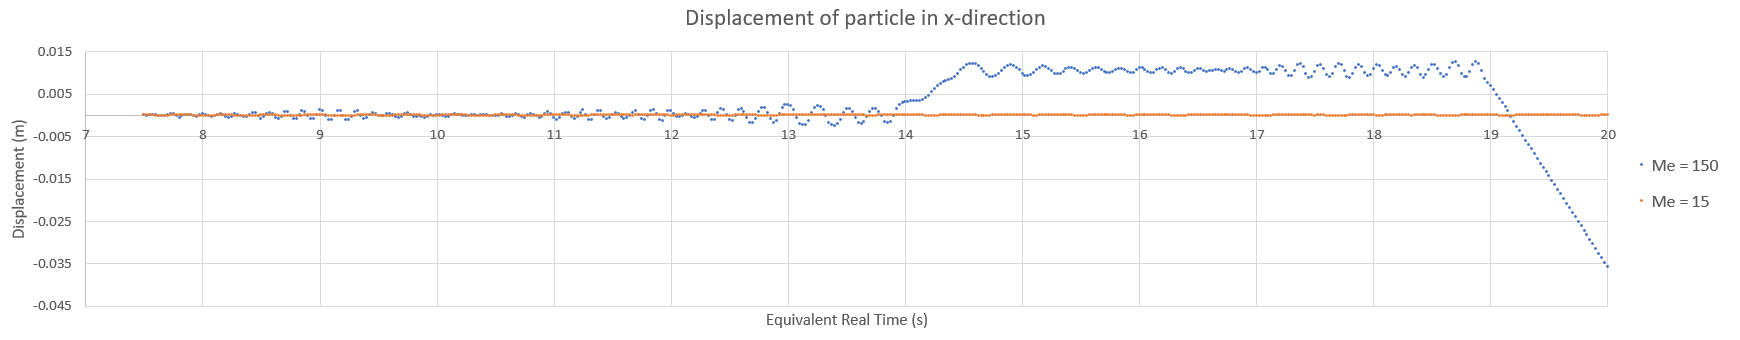
\includegraphics[width=\textwidth]{simulation/highmemory/displacement.png}
		\caption{Graph of displacement in the x-direction over time. $Me=150$ represents the high memory regime, whereas $Me=15$ represents the low memory regime}
		\label{fig:mem:displacement}
	\end{subfigure}
	
	\begin{subfigure}{\textwidth}
		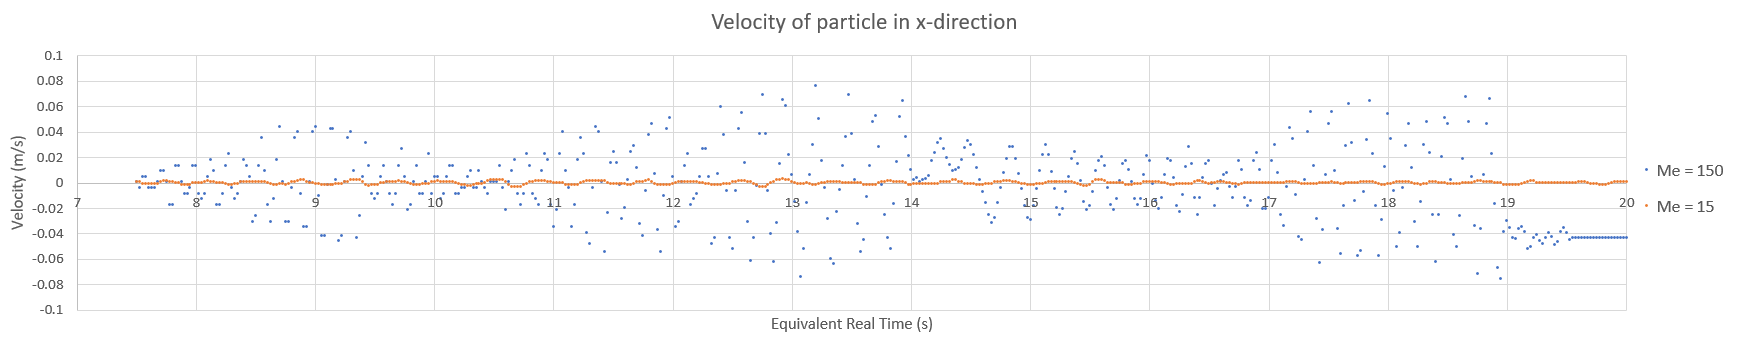
\includegraphics[width=\textwidth]{simulation/highmemory/velocity.png}
		\caption{In the high-memory regime, the particle velocity fluctuates chaotically before entering a stable state $\approx 11$s after perturbation. In the low-memory regime, the particle has negligible velocity}
		\label{fig:mem:velocity}.
	\end{subfigure}
	
	\begin{subfigure}{0.475\textwidth}
		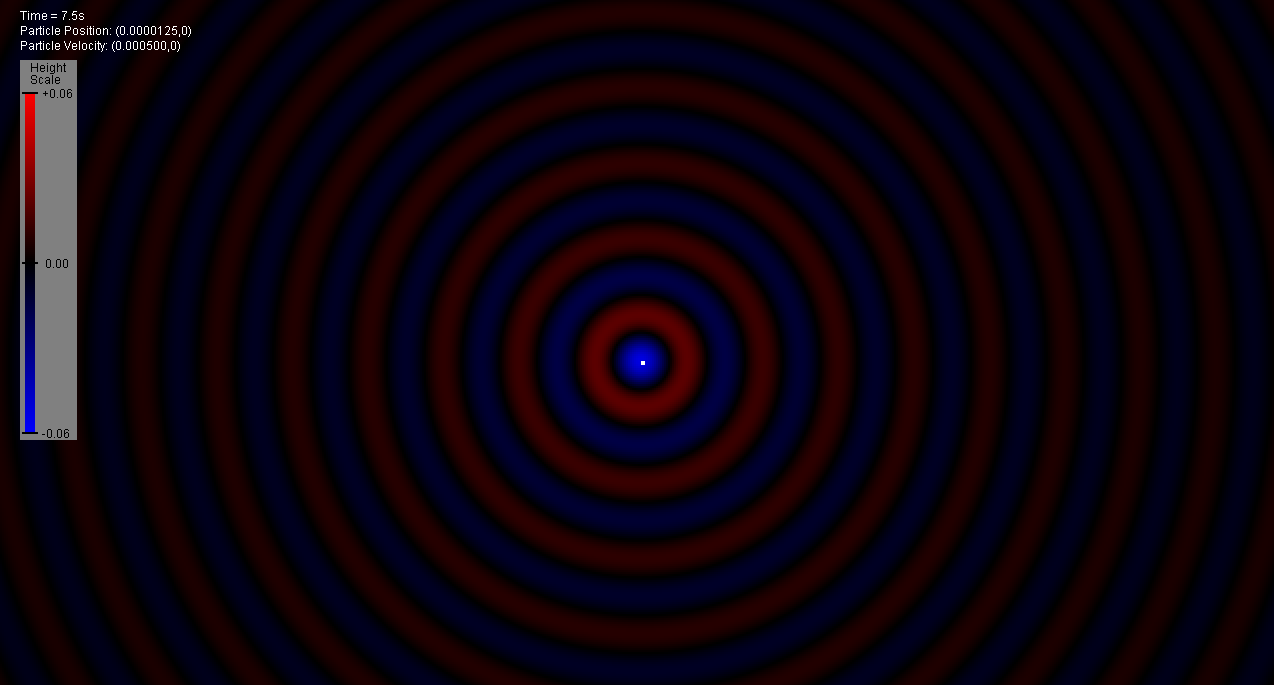
\includegraphics[width=\textwidth]{simulation/highmemory/wavefield75.png}
		\caption{The overall surface wave after $7.5$s; the wave-field has a similar shape to a 2-D harmonic potential well}
		\label{fig:mem:wavefield75}
	\end{subfigure}
	\hfill
	\begin{subfigure}{0.475\textwidth}
		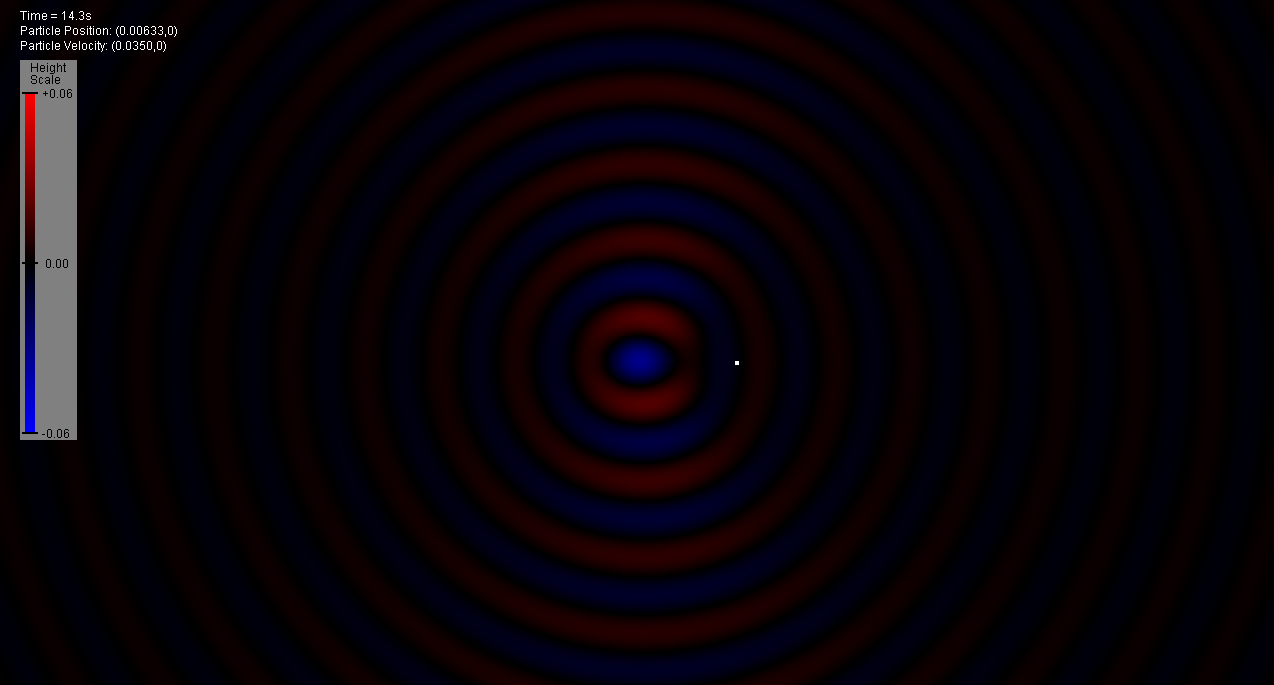
\includegraphics[width=\textwidth]{simulation/highmemory/wavefield145.png}
		\caption{The wave-field at $14.5$s, just prior to the particle breaking through the potential barrier and travelling}
		\label{fig:mem:wavefield145}
	\end{subfigure}
	
	\begin{subfigure}{0.475\textwidth}
		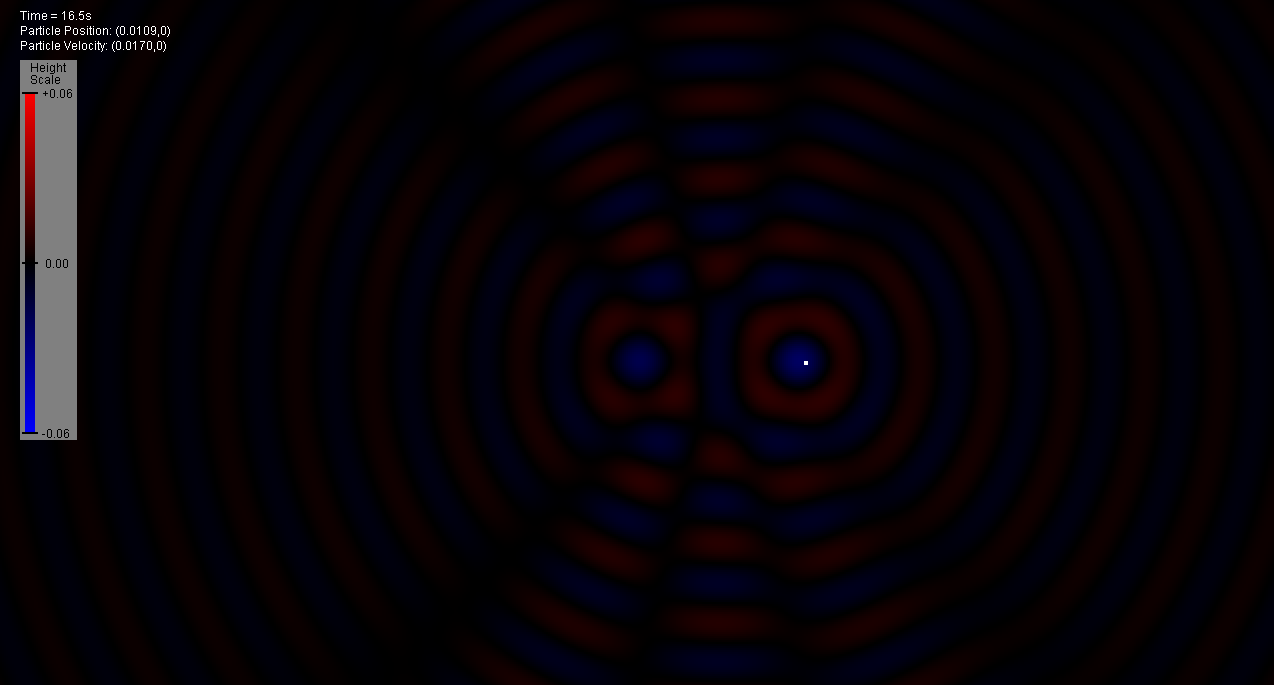
\includegraphics[width=\textwidth]{simulation/highmemory/wavefield165.png}
		\caption{Following multiple interactions with wave peaks, the particle decelerates and reforms a potential well}
		\label{fig:mem:wavefield165}
	\end{subfigure}
	\hfill
	\begin{subfigure}{0.475\textwidth}
		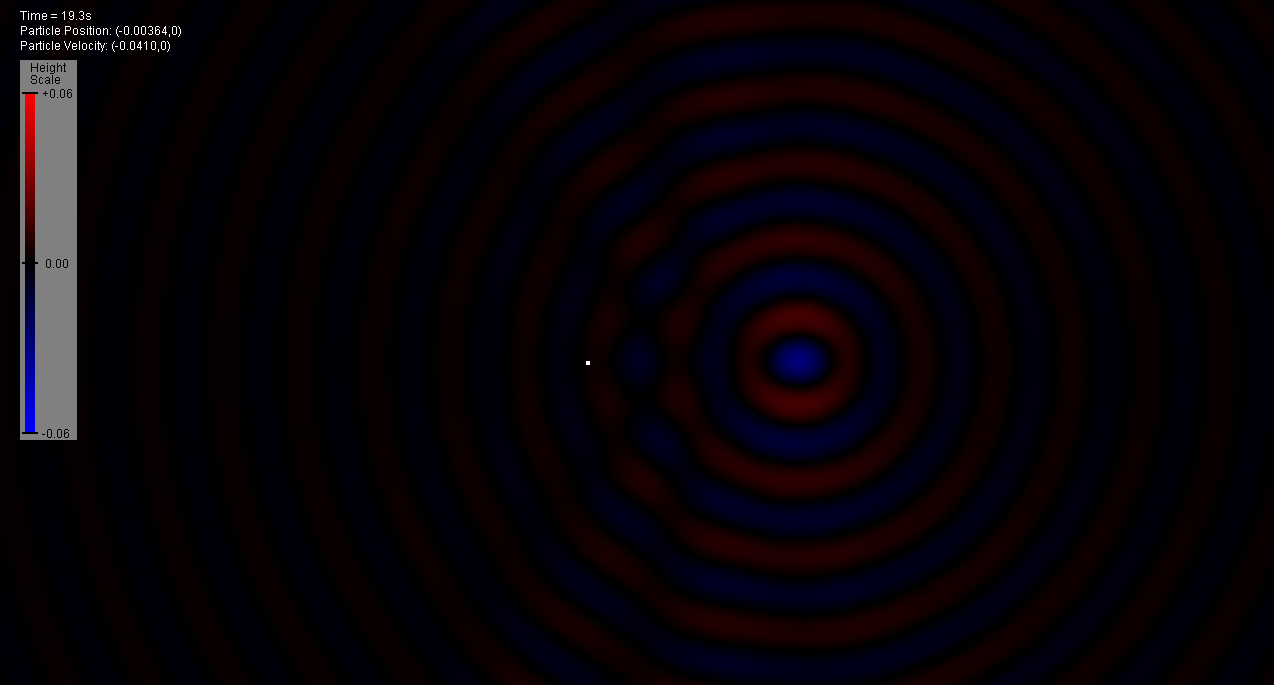
\includegraphics[width=\textwidth]{simulation/highmemory/wavefield195.png}
		\caption{The stable wave-field at $19.5$s, now displaced by $0.01m$.}
		\label{fig:mem:wavefield195}.
	\end{subfigure}
\caption{Results of the simulation in the high- and low-memory regime at different time periods}
\label{fig:memory}
\end{figure}

We see from Figure \ref{fig:mem:velocity} that the particle velocity is chaotic. This causes the particle to oscillate around two centres of displacement, initially the start position, and later about the point $(0.01,0)$. We also observe in Figure \ref{fig:mem:wavefield75} that, prior to perturbation, the wave-field is similar in shape to a 2-D harmonic potential well, of width $\lambda/2$, and centred about the initial position of the particle. Upon perturbation, the particle oscillates, as expected for such a system. However, with each impact at positions away from the start position, new waveforms are added to the overall wavefunction at these points. The waves formed at this point superpose over the 2-D harmonic potential well, flattening it along the x-axis. After approximately 7s, the peaks at $\lambda/2$ away from the start position along the x-axis were low enough that the particle could leave the well as shown in Figure \ref{fig:mem:wavefield145}.

The overall surface wave at 7.5s is shown in Figure \ref{fig:mem:wavefield75}. The wavefield is observed to be similar in shape to the 2-D harmonic potential well within a half wavelength about the particles' start position. At this point, the particle is perturbed. As expected for a particle oscillating in a 2-D harmonic potential, the particle enters oscillatory motion. However, with each impact at positions away from the start position, new waveforms are added to the overall wavefunction at these points. The wave forms at this point superpose over the 2-D harmonic potential well flattening it along the x-axis. After approximately 7s, the peaks at half wavelength away from the start position along the x-axis were low enough that the particle could traverse it and leave the well about the start position. The overall surface wave at this point is shown in Figure \ref{fig:mem:wavefield145}. As the particle carries on in its trajectory away from the start position, it interacts with other smaller peaks, causing it to slow down. As the particle slows down, the most recently formed waves are centered closer and closer together, eventually reforming yet another potential well about the point (0.01,0). The overall surface wave at this point is shown in Figure \ref{fig:mem:wavefield165}. The particle then starts oscillating about this point for approximately 4s before the same mechanisms that allowed it to break through the first potential well occurs, and the particle leaves the new formed well. Following this the particle enters a steady state and continues travelling with a stable velocity of (-0.043,0) $ms^{-1}$. The particle has thus started ``walking".

The high memory regime simulation was repeated for perturbation velocity with magnitude between 0.0001 $ms^{-1}$ and 0.0020 $ms^{-1}$ at intervals of 0.0001 $ms^{-1}$, to ensure that the above result of achieving walking was not due to specifically selected variables. In all cases the particle entered a steady ``walking" state with velocities ranging form magnitude 0.00859 to 0.102. The final steady state velocities of each particle and their corresponding perturbation velocity can found in \ref{fig:pertVfinal}. No observable trend was found relating the steady ``walking" state velocity and the perturbation velocity.
\begin{figure}
    \centering
    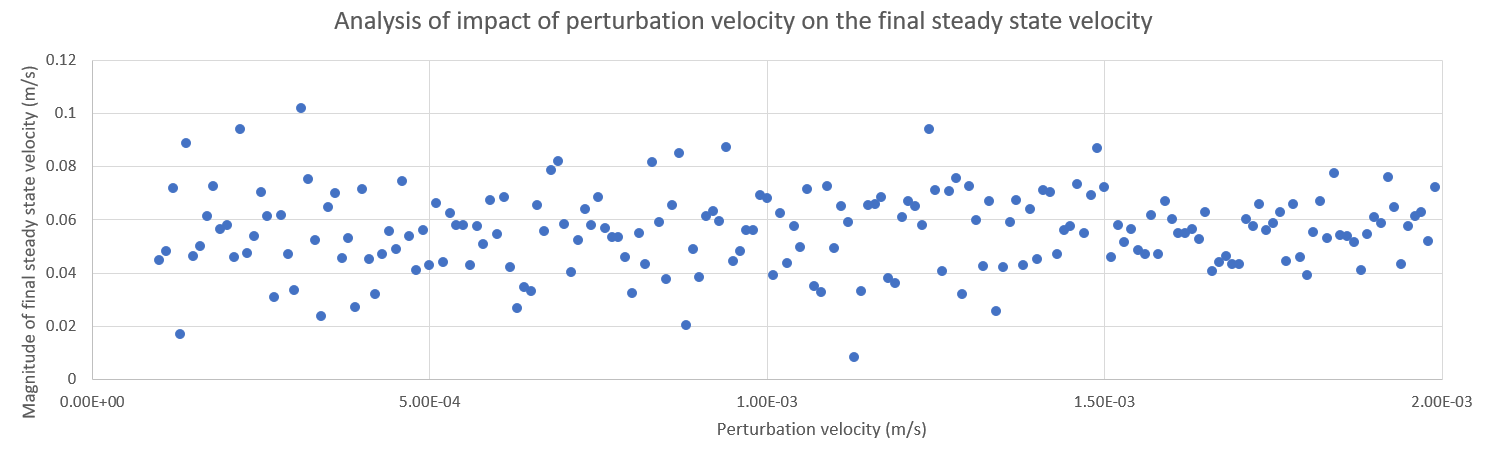
\includegraphics[width=\textwidth]{simulation/figpert.png}
    \caption{Results of the simulations in the high memory regime at velocities ranging from 0.0001 $ms^{-1}$ and 0.002 $ms^{-1}$}
    \label{fig:pertVfinal}
\end{figure}

The above results strongly suggest that a particle entering the walking state depends on $Me$. Simulations were next conducted for $Me$ between 15 and 150 at intervals of 0.1. Perturbation velocity was kept constant at (0.0005,0) $ms^{-1}$ in all simulations. The following conditions were set to determined if the particle has entered a walking state:

\begin{enumerate}
    \item $\Delta\vec{v} = 0$ for the past 20 time steps.
    \item The particle is at least 1 wavelength away from where it was initiated.
\end{enumerate}

If the particle in a simulation was detected to be in a walking state, the simulation would output the walking state velocity and the time at which "walking" was achieved. Each simulation was allowed to run for 10,000 time steps, corresponding to 250s in real time. Any particle yet to achieve walking within this time frame was assumed to not be capable of entering the walking state. Visualisations of this data are shown as graphs in Figure \ref{fig:varmem}. 

As shown in Figure \ref{fig:varmem:walkingstate}, there is no clear threshold $Me$ beyond which the particle will enter a walking state. From the plot it is observed that walking will not occur for $Me < 50$ but will occur for $Me > 80$. The region in between, given by $50\leq Me\leq80$, however, appears to be a grey area where whether a given Me leads to a walking state seems to follow some distribution. To determine the shape of this distribution a moving average of the previous 20 and next 20 points was plotted against $Me$. By observation, the plot here appears to be in the shape of a sigmoid curve. Using Origin Pro 2017s' non-linear curve fit function, the plot in was fitted to a Boltzmann sigmoid function with the top and bottom value fixed at 1 and 0 respectively. The Boltzmann sigmoid is given by \ref{equ:BoltzmanSigmoid}.

\begin{equation}
y = (bottom) - \frac{(top)-(bottom)}{1+exp \frac{\left(x_0 - x \right)}{dx}}
\label{equ:BoltzmanSigmoid}
\end{equation}

Here $x_0$ is the 50\% threshold found to be $64.54\pm0.04$.

The fit was found to have a R-squared value of 0.9974 and a reduced chi squared value of $5.33 \times 10^{-4}$ suggesting a decent fit. The plot of the residual of the fit against $Me$, as shown in Figure \ref{fig:varmem:residualplot}, interestingly seems to be in the form of a wave packet. 

Figure \ref{fig:varmem:timewalking} shows the relation between time taken to enter the walking state and $Me$. It is observed that the time taken has a wider spread for lower Me, with a minimum that remains constant as Me increases. The minimum has a value of approximately $3\pm2$. This corresponds to the time required to flatten the sides of the wave as described previously, thus allowing the particle to pass through it and leave the potential well around it.

The plot of the x-component of the walking velocity against $Me$ is shown in Figure \ref{fig:varmem:walkingvel}. Since the particle was perturbed in the x-direction only, the y-component in all cases is 0. It is observed that approximately half of the simulations produced a walking velocity in the positive x-direction (the direction of perturbation), while the remaining half in the negative x-direction. 



\begin{figure}
	\centering
	\begin{subfigure}{\textwidth}
		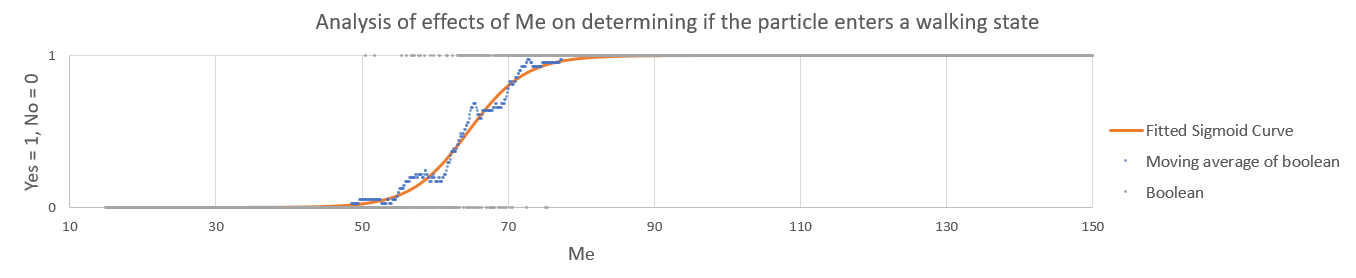
\includegraphics[width=\textwidth]{simulation/varmemory/walkingstate.png}
		\caption{Binary plot showing whether a particle was found to have entered a walking state within 10,000 time steps with 1 corresponding to yes and 0 to no against $Me$. The moving average is plotted and fitted to a sigmoid curve}
		\label{fig:varmem:walkingstate}
	\end{subfigure}
	 \begin{subfigure}{\textwidth}
		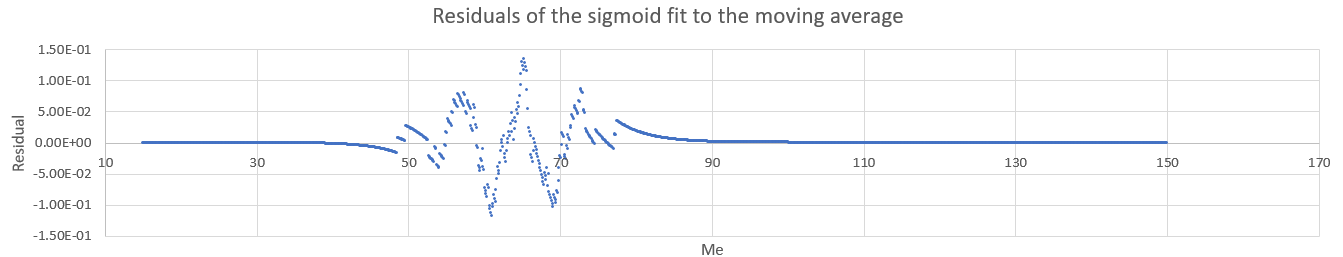
\includegraphics[width=\textwidth]{simulation/varmemory/residuals.png}
		\caption{Residual plot of the sigmoid fit of \ref{fig:varmem:walkingstate}}
		\label{fig:varmem:residualplot}
	\end{subfigure}
	\begin{subfigure}{\textwidth}
		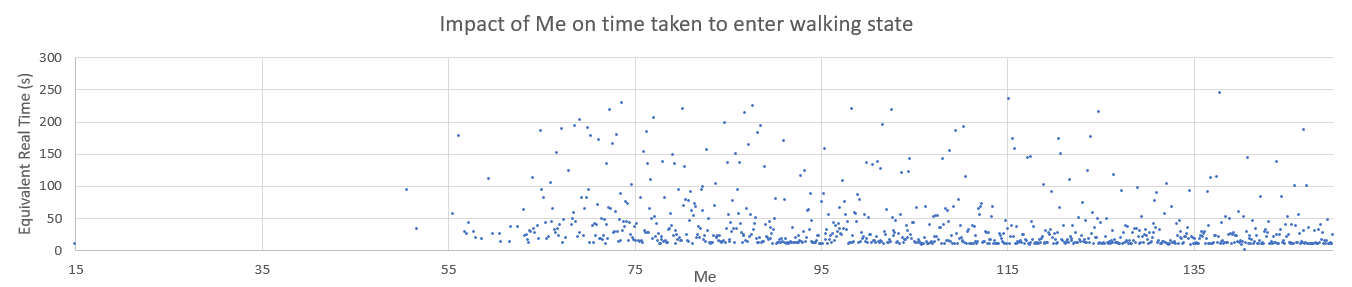
\includegraphics[width=\textwidth]{simulation/varmemory/meWalkingState.png}
		\caption{Plot of time taken for the particle to enter walking state against $Me$ used in the simulation}
		\label{fig:varmem:timewalking}
	\end{subfigure}
	
	\begin{subfigure}{\textwidth}
		\includegraphics[width=\textwidth]{simulation/varmemory/velocityWalkingState.png}
		\caption{Plot of walking velocity of the particle against $Me$ used in the simulation}
		\label{fig:varmem:walkingvel}
	\end{subfigure}
\caption{Analysis of the probability of a particle entering the walking state at different values of $Me$}
\label{fig:varmem}
\end{figure}

\subsection{Preliminary tests on predicted phenomena}
The theoretical models used in our simulations also made other predictions as to the behaviour expected. To further provide supporting evidence for the validity of our  assumptions, we attempted to demonstrate some of these predictions. Due to time constraints, we only managed to run preliminary tests demonstrating oscillating droplets and wall repulsion.

\subsubsection{Oscillating droplets}

As predicted, \cite{brady2014bouncing} bouncing droplets experience an attractive force when they are bouncing in phase. Experimental evidence provided by the same team suggests that this force follows an inverse square relation similar to gravity and electromagnetism. A preliminary test was conducted by performing a simulation that initiated two droplets, separated along the x-axis by 0.004m. The droplets were initiated with velocities in the y-direction with magnitude 0.0003 $ms^{-1}$ in opposite directions. This resulted in the droplets having an angular orbital momentum between themselves.

In the simulation performed, it was observed that the droplets initially entered some form of orbital motion, as expected from an attractive inverse square force. However, orbital motion was only maintained for an equivalent real time of approximately 6s before the system destabilises. The droplets were then observed to enter walking states in opposite directions. Due to time constraints, further detailed analysis on the motion of the droplets were not performed. 

\subsubsection{Wall repulsion}

Wall repulsion was simulated by initiating a droplet displaced along the positive x-direction. A wall was positioned along the y-axis. By assuming the wall is completely reflective, an incoming wave should reflect off the wall out of phase, and in the direction given by the law of reflection. To simulate this, inspiration was taken from the method of mirror charges in electrostatics. Each time a waveform was added to the overall wave-function, a “mirror” waveform was also created. The “mirror” waveform added was out of phase with the droplet, and initiated at the position given by the reflection of the droplet in the y-axis.

The simulation demonstrated that the droplet accelerates away from the wall, as expected. Due to time constraints, no detailed analysis was performed on the motion of the particle so the trajectory of repulsion was not quantified. The effects of changing variables was also not explored.


\subsection{Conclusion}

The original aims of the simulation were to construct an interactive software package that could simulate and visualise the motion of droplets bouncing on a liquid surface. These aims were partially met: a non-interactive simulation was developed, whereby images from the software output could later be reconstructed into a video. However, due to computational limitations it was not possible to run this process in real time. This posed a significant barrier to the use of the simulation as a real-time educational aid, although the videos were still useful to illustrate the concepts to students in a classroom.

As work continued with the simulation, and the team developed a more detailed understanding of the theory behind droplet motion, additional goals were added to the project. This included determining the effect of changing simulation parameters such as the memory coefficient $Me$, and allowing the end-user to vary those without needing to understand the source code. Again, these were partially met: detailed analysis of the effect of $Me$ has been offered, an insight which would not be possible within the physical system. However, simulation parameters are still hard-coded, although this could change with relative ease in the future.

While a more quantitative analysis of boundary conditions and multiple droplets would have been desirable, the preliminary results obtained agreed with qualitative predictions. This suggests the simulation's behaviour is consistent with theory, but without quantitative comparisons, the accuracy of this could not be verified. This meant that the subsidiary goal of representing quantum effects, such as double-slit diffraction, was not met. To provide a more accurate model, several other factors that were assumed negligible could be accounted for, such as adding a parameter to represent the inelasticity of collisions between the droplet and the surface.

\clearpage

\section{Education and outreach efforts}
Having developed a portable prototype of the apparatus, investigations into its use as an educational tool were started. The aims of this part of the project were to identify the ability range of students who could benefit from such outreach, to develop and implement an outreach lesson, and assess its effectiveness in engaging students in undergraduate physics.

Considering the relatively high level of understanding of quantum physics required to grasp both the theory behind our experiment and its implications, sixth-form students were selected as the primary target group. To that end, teachers at schools project members had attended were contacted, and a school in Chesham selected for an outreach lesson. A lesson plan (Section \ref{lessonplan})) was developed, with significant feedback from Dr. Mark Fuller, outreach officer for the department. This, alongside a Powerpoint (Appendix \ref{app:powerpoint}), was delivered on the 7th March.

Evaluation of the lesson was conducted through a paper survey, overleaf, and through feedback from the class teacher. Students used a four point rate their agreement with various statements corresponding to our outreach aims. Each statement was then assigned an "agreement score", defined as $\frac{\sum{x}}{4N}$, where x is the score given to each statement and N is the number of students in the class. The results of this are shown in Figure \ref{fig:evaluationchart}.

\begin{figure}[h]
\centering
\includegraphics[width=\textwidth]{education/evaluationchart.pdf}
\caption{Percentage agreement with evaluation statements. Note that the final statement included a "not applicable" option, so has a smaller sample size.}
\label{fig:evaluationchart}
\end{figure}

This evaluation showed that students generally found the lesson enjoyable and engaging, and valued the use of the prototype as a demonstration aid. Understanding of the quantum effects shown by our experiment was less robust, although this could be due to the year 12 students being unfamiliar with such topics beforehand, as they don't study quantum physics in detail until year 13. Most lacking from this intervention was an understanding of the experience of studying physics at university. It would be relatively easy to devote more time to this in future sessions, depending on the precise aims of the workshop, which should provide sufficient improvement.

\clearpage

\subsection{Lesson Plan} \label{lessonplan}

\noindent Date: 7/3/18

\noindent Lesson: Physics

\noindent Year: 12/13

\noindent Levels: Any

\noindent Tutor: Group 13

\noindent Topic: Quantum mechanical effects using bouncing droplets


\noindent Learning objective and outcomes:
\begin{enumerate}
\item How droplets can bounce on a vibrating surface
\item What quantum mechanics is, and what effects we can observe some of these things from the apparatus
\item Have an insight into undergraduate physics and some of the hands on work it can entail
\end{enumerate}

\noindent \textbf{Introduction} (5 mins): Introduce ourselves and the reasons we're there for. 

\noindent \textbf{Starter} (10 mins): Start discussion into what quantum physics is. To facilitate audience participation, ask students to discuss amongst themselves for 3 minutes and propose ideas. Then ask for these ideas, and add/correct responses as required

\noindent \textbf{Mini-lecture} (10 mins): How do droplets form? (Diagram on board) Explain that (but not how) these droplets demonstrate QM behaviour. Starting from basic diagrams and maybe a recording of bouncing droplet motion, explain how droplets bounce. Then explain that these droplets replicate quantum behaviour. Attempt to limit the scope of this behaviour by mentioning specific effects. Don't explain how this link occurs yet.

\noindent \textbf{Demonstration} (10 mins): Explain apparatus and highlight important components. Execute a run through of the apparatus (need to find a way to get a live feed to projector). Specifically demonstrate bouncing droplets, walking droplets and multiple droplet motion. Take time to allow for students to run through experiment themselves, e.g. by making droplets and playing with the frequencies/bass. As there is only one apparatus, take suggestions from students. 

\noindent \textbf{Discussion} (10 mins): Discuss in groups how these droplets display behaviour. Ask students to also note down any interesting behaviours they observe. May have to use lab based recordings/ simulation for double slit diffraction or other interesting effects we want to mention

\noindent \textbf{Plenary} (10 mins): Assert that droplets demonstrate XYZ behaviour, make limitations clear. Wrap up by emphasising learning objectives, link to Veritasium for more details. It would be quite useful to part on an entertaining note. See if music/ colourful lights can make the apparatus do something more exciting. 

\noindent \textbf{End of session} (10 mins): 10' Q&A on Physics at Uni, completion of end of session assessments. 



\noindent \textbf{Key words}: Pilot wave theory, guiding wave equation, wave particle duality, Destructive and constructive interference

\includepdf{education/evaluation.pdf}

\clearpage
\section{Project Proposal}
The following section is a draft proposal to be put forward to the  Science and Technology Facility Council, in hopes of winning the Public Engagement Spark Award, which will award us with extra funding to extend our project, and fully accomplish our outreach goals. 
\subsection{Aims}

Our project aims to inspire the next generation of physicists and, in particular, secondary school students in the United Kingdom. We hope that students will form a more positive attitude towards STEM subjects. More precisely, our aim is to help students get a unique insight into quantum mechanics, therefore making the subject much more exciting and intuitive. We will achieve this by providing equipment with which the visualisation of complex quantum mechanical phenomena is made possible on a macroscopic level.

As part of our third year group project at University College London, we have assembled an apparatus with which the visualisation of quantum mechanical effects is possible. This consists of a woofer, on which a petri dish containing washing liquid is placed. The woofer drives the air under the petri dish which makes the surface of the oil vibrate too. With careful calibration of this apparatus, it is possible to make droplets, which vibrate above the immediate surface. A high-resolution photo of a bouncing droplet can be seen in Figure 1. These oil droplets behave exactly how the pilot-wave theory predicts how quantum particles should behave. Pilot-wave theory explains the behaviour of quantum particles ingeniously: it suggests that they consist of the particle itself and its pilot wave. When we see particle-like effects, we see the particle interacting, and when we see wave phenomena, the pilot wave is interacting with its own reflections. This can be imagined just like the particle and its wave in Figure \ref{fig:droplet_STFC_report}. Numerous quantum mechanical phenomena can be demonstrated and visualised using this apparatus, including the double-slit experiment or even a molecule-like structure of two particles. Simulations were also made as part of this project, to see how well prediction and experimentation agree in this case.  

\begin{center}
\begin{figure}[htb]
\centering
    \includegraphics[width=8.996cm,height=5.997cm]{education/STFCproposal/Droplet_STFC.jpg}
    \caption{An image of a bouncing droplet captured mid-oscillation.}
    \label{fig:droplet_STFC_report}
\end{figure} 
\end{center}

In the public's view, quantum physics is a mysterious and unpredictable world. This apparatus provides an excellent opportunity to alter their perception and increase public engagement with quantum mechanics. Not only does it show numerous aspects of quantum mechanics, but also it helps make it seem less distant to people. It shows young students that, using the power of science, even such a strange world can be understood and manipulated.

Investigation of quantum phenomena is a significant proportion of today's physics research. To make students more familiar with quantum mechanics is essential to maintain, or even raise, the number of students choosing a science-related career.

Our eventual goal is to develop a compact product, with which bouncing oil droplets can be made, and to present it in schools. Potentially, depending on the demand, the apparatus can be manufactured and given or sold to schools, to enable them to conduct their own experiments in order to encourage their pupils' curiosity. 

\subsection{Objectives}

We have three key objectives: perfecting the apparatus and our simulations, carrying out market research and delivering to schools. We plan to aim this apparatus towards students in years 10 and 11. During this time period they are just about to choose their A-level subjects, and therefore the most impact can be made. They are also old enough to understand some basic concepts of modern science.

\begin{center}
\begin{figure}[htb]
    \centering
    \includegraphics[width=0.7\textwidth]{education/STFCproposal/STFCProposal_Timeline2.png}
    \caption{A brief timeline of the planned project so far, once STFC funding has been granted}
    \label{fig:PropTimeline_STFC}
\end{figure} 
\end{center}

Figure \ref{fig:PropTimeline_STFC} shows how long each portion of the project will last. According to our initial plan, the project should last 5 months. After this period, we will evaluate feedback that we have collected from the schools and look for ways to carry out improvements.

\begin{enumerate}
\item \textbf{Perfecting Apparatus}

The apparatus that we have assembled as part of our group project is rather robust and not easily movable. It consists of the following parts: loudspeaker (woofer), rigid wooden plate, fold back clippers, wires with crocodile clip, amplifier power supply cable, synchronized function generator, BNC cables and 6.5'' petri dish. We have tried silicone oil as liquid in the petri dish, however, from our experience, water mixed with soap is a better and cheaper alternative.

We wish to improve this apparatus so that all parts can be contained by a compact wooden box. This will make the device easy to move and also look more professional. The device can also be used also with a smart phone serving as a function generator, which would enable some room for interaction with students. To achieve this, we have to make some small modifications to the set up. A schematic of a possible version of this apparatus can be seen in.  \ref{fig:apparatus_diagram_STFC}.

\begin{figure}
\centering
    \includegraphics[width=16.14cm,height=9.647cm]{education/STFCproposal/Apparatus_STFC.png}
    \caption{Potential apparatus setup, post improvements and granting of STFC funding.}
    \label{fig:apparatus_diagram_STFC}
\end{figure}

We have also made simulations which demonstrate how quantum particles should behave according to pilot-wave theory. Due to the limited amount of time, these simulations are rather simple. However, in the future, these could be made into short films to show to students.

In addition, we have recorded footage of the bouncing droplets using an ultra-high speed camera. This enables the viewers to have an even more detailed look at these phenomena and really see what is happening step by step.


\item \textbf{Market Research}

We think that it is extremely important to properly investigate the potential this project has. This will firstly consist of determining the exact age-group that we wish to aim this project at and finding and contacting as many schools as possible to see if they are interested in hosting us as outreach speakers.

In order to have a significant impact on the long-term decisions that students make, it is crucial to find the adequate age-group that we mainly want to outreach to. If the students are too old, the impact on them is significantly smaller, on the other hand, if they are too young, they might not have the technical knowledge that is required to fully grasp the experiment. We hope to find the critical phase in the students' life when they are yet to decide how to continue their studies, but they are already aware of the existence of quantum mechanics.


\item \textbf{Outreach to Schools}

Using our prototype, we have visited a school already (Chesham Grammar school), as a trial for or long-term plan. From our experience, students found the apparatus to be eye-catching and innovative. We made preliminary feedback forms which were given to the students we presented to. The results are unanimous: 95\% of the students found the demonstration useful in understanding the quantum world, and more than 60\% of them were more interested in studying physics in the future after the demonstration. 

We are also planning to make a non-technical script which enables anyone to construct the device. This would include an equipment list, a building guide experiments and lesson plans that anyone can carry out using the device.

In addition to these, we also want to produce a short video in which we would explain the phenomena and demonstrate how to produce, manipulate and experiment with the bouncing droplets. \ 

\end{enumerate}

\subsection{Summary}

We will produce a compact apparatus which is easily movable and demonstrates quantum mechanical phenomenon using bouncing droplets. Then, we will contact schools, potentially with the help of STFC, to find possible platforms where we can demonstrate our project. We will ask the participating students and teachers for feedback and improve accordingly. 


\bigskip

\subsection{Project Personnel}

Steven Vuong and Kelvin Fang will be responsible for the improvement of the apparatus and its branding. Steven will make sure that the device is compact and easy to use and Kelvin will ensure that the apparatus is visually appealing. In addition, they will try to reduce the cost of the equipment as much as possible, thus making it more affordable. Furthermore, they will also seek external consultants (designers and engineers) to obtain expert opinions for further improvements.

Georges Ajaka and Alex Stock will further develop simulations of the quantum effects that can be visualised using the device. This job requires a high level of programming skills so, in the future, the help of an expert might be necessary. The simulation will hopefully enable the students to see similarities between the quantum world and bouncing droplets. We are planning to make the code they produce open-source.

The market research will be conducted by Chong Keat Gea and Benjamin Berczi. They will contact schools to gauge interest in this outreach opportunity. Then, surveys would be sent to the schools that are interested. These surveys will contain questions about what would interest the students and what they would prefer to see during a demonstration, along with the technical understanding of physics possessed by their average student. 

After conducting the market research, Johnny Allain-Labon and Mohit Motwani will visit schools that expressed interest and demonstrate our device in person. They will work alongside STFC associates to deliver an hour long demonstration. Johnny and Mohit have already prepared a guest lesson plan and an evaluation form for it as well, with the assistance of the Physics Department outreach officer, Dr. Mark Fuller. 

\subsection{Related Activities}

There are many papers about this phenomenon and there has been several attempts to use it as a tool for public engagement. However, we feel that its potential hasn't been fulfilled. Examples of papers published on this topic include:
\begin{enumerate}
    \item J. Walker. Drops of liquid can be made to float on the liquid. What enables them to do so? Sci. Am, 238(6):123--129, 1978
    \item Y. Couder, S. Proti\'ere, E. Fort, and A. Boudaoud. Dynamical phenomena: Walking and orbiting droplets. Nature, 437(7056):208--208, 2005.
    \item R. Brady, R. Anderson. Why bouncing droplets are a pretty good model of quantum mechanics \url{https://arxiv.org/abs/1401.4356}
\end{enumerate}

In terms of public engagement, attempts have been made using YouTube. The most viewed YouTube video on this topic is by Veritasium: ``Is This What Quantum Mechanics Looks Like?'', \url{https://www.youtube.com/watch?v=WIyTZDHuarQ\&t=185s}. 

Although this video demonstrates the similarities between the bouncing droplet phenomenon by referencing papers, it does not show how droplets are made and how they behave. In addition, it doesn't make efforts to explain the physics of it in detail for the younger groups of audience. 

\subsection{Awareness raising, dissemination and networking}

We hope to raise awareness by giving the public a closer look at modern science; by making quantum mechanics more visual. We hope to influence adults as well as students. The project's main aim is to have an impact on students, however, using social media, adults can be reached too. 

During the demonstrations in schools, students will get an insight of how quantum mechanics works and how it can be manipulated. 

In addition, we plan to upload our video, in which we demonstrate our project, to Youtube as well. Youtube provides us access to a widely used platform with which we can reach many people from different backgrounds.

Moreover, students will be able to network with us, university students, and also STFC associates to gain knowledge about their options in science. 

\subsection{Monitoring and Evaluation}

As mentioned before, we will use feedback forms and surveys to gain audience feedback. These forms will be processed and evaluated by the market research team. They will enable us to make improvements in order to make our product more relatable and exciting. 

YouTube provides us with immediate feedback as well, with which we can get an impression of the experience that people of all ages get. This will help improve the apparatus and presentation to a wider range of audiences. 


\subsection{Justification of Resources}
\bigskip
\begin{table}
\centering
\begin{tabular}{|c|c|c|c|}
\hline
\textbf{Category}& \textbf{Product} & \textbf{Cost(\pounds)} & \textbf{Source} \\
\hline
\multirow{10}{4em}{Apparatus} & Loudspeaker & \pounds25 & Amazon\\
& Amplifier (with power supply cable) & \pounds18 & Amazon \\ 
& 4" Petri dish & \pounds3 & Amazon\\
& LED strips & \pounds9 & Amazon\\
& Mini-Jack cable & \pounds6 & Amazon\\
& Glue and Paper & \pounds3 & Ryman\\
& Clippers & \pounds5 & Hardware store\\
& Wooden plate & \pounds3 & Hardware store\\
& Kitchen soap & \pounds2 & Tesco\\
& \textbf{Category Cost} & $ \pounds74 \times 10= \pounds 740$ &  \\
\hline
\multirow{3}{4em}{Camera} & Sony DSCRX100M4 & \pounds792 & Amazon\\
& 4'' Hama Star 61 Camera Tripod & \pounds3 & Amazon\\
& \textbf{Category Cost} & \pounds814 &  \\
\hline
\multirow{3}{4em}{Personnel} & Designer & \pounds1500 &  \\
& Engineer & \pounds1000 &  \\
& \textbf{Category Cost} & \pounds 2500 &  \\
\hline
\textbf{ }& \textbf{Grand Total} & \textbf{\pounds4054} &   \\
\hline

\end{tabular}
\caption{Details of the projected cost for developing the outreach project further, inluding section by section costs}
\label{table:STFC_costs}
\end{table}
\bigskip

The costs to build the prototype we have constructed part by part can be seen in \ref{table:STFC_costs}. It can be seen that it costs approximately {\pounds}74 to build our apparatus. From the wooden plate a wooden box can be constructed using laser printing -- which is available for us, UCL students at the Institute of Making. The kitchen soap mixed with water can replace the silicone oil in the experiment, which lowers the costs. 

In the first round of our plan, we want to visit and supply a minimum of 10 schools, in order to gain a sufficient amount of feedback for future improvements. This would mean 10*{\pounds}74={\pounds}740.

In addition, we require a high-speed camera to record excellent quality footage as explained before. We also need a camera stand which allows for the camera to be held steady.

Moreover, we plan to involve external personnel in the project: an engineer and a designer. We would employ them for about two weeks. The ratio of the average salary for a designer to an engineer is about 1:1.5. Therefore the salaries we offer have the same ratio.

In conclusion, we require {\pounds}4054 to conduct our project and reach schools in the UK, in order to improve public engagement regarding STEM stubjects.


\section{Conclusion}

In conclusion, only some of the initially stated aims and objectives were accomplished. A basic, table-top version of the apparatus created by \textit{Couder et al.} was developed. This apparatus was capable of displaying bouncing, walking and orbiting motion. However, due to time constraints more complex behaviours such as double slit diffraction, were not demonstrable. A suitable programming language was identified, and initial forays into developing a computer simulation were made. Observations from the computer simulation agreed well with the experiment, which suggested the validity of the mathematical model used. More numerical analysis is needed to further confirm this. A pilot outreach lesson with year 12 students was conducted, with generally positive feedback obtained.

If this project were to be pursued further, with additional resources, further investigations into displaying quantum phenomena with the apparatus could be made. Primarily, phenomena such as double slit diffraction and quantum tunnelling with droplets will be demonstrated, as these allow for more tangible links to be made with quantum mechanics. Quantitative analysis, to definitively verify the mathematical model, alongside development of a standalone version of the simulation is also an another avenue to pursue. In particular, a standalone simulation usable in classrooms would be particularly advantageous, as it allows for increased interactivity, ensuring more effective student engagement. Although the initial outreach efforts were successful, more feedback is necessary from a wider variety of schools in order to make well-supported improvements. If the draft STFC proposal introduced in the report is successfully approved, additional resources will be available for further outreach efforts, and for more effective purpose-oriented improvements to the apparatus such as branding. 
\clearpage

\clearpage
\bibliographystyle{IEEEtran}
\bibliography{bibliography.bib}
\clearpage


\begin{appendices}

\noindent 
\section{Minutes 11/1/18}\label{app:11-1}

\noindent Meeting Time: 4pm Thursday 11th Jan

\noindent Meeting Location: Massey Group Study Pod, 3rd Floor, Science Library
\\\\
\noindent \textbf{\underbar{Attendance}}

\noindent Chair: Chong Keat Gea CKG

\noindent Vice-Chair: Kelvin Fang KF

\noindent Secretary: Johnny Allain-Labon JAL

\noindent Treasurer: Mohit Motwani MM

\noindent Georges Ajaka GA

\noindent Course Coordinator Point of Contact: Steven Vuong SV

\noindent Benji Berczi BB

\noindent Alex Stock AS

\noindent Prof. Ryan Nichol RN

\noindent 

\noindent Present: CKG KF JAL MM GA SV BB AS RN

\noindent 
\\
\begin{enumerate}
\item  \textbf{Project Outline}

\begin{enumerate}
\item Existing equipment: none, constructing prototype from scratch

\item  Prototype - start as simple as possible e.g. petri dish on loudspeaker e.g. \url{https://www.youtube.com/watch?v=WIyTZDHuarQ}.  Move on to more complex behaviour if possible

\item  Simulation Programme - want to demonstrate quantum behaviours of the bouncing oil drops if experimental verification is problematic + add missing features of experiment.\\
\end{enumerate}

\item  \textbf{Aims \& Objectives}

\begin{enumerate}
\item Construct prototype:

\begin{enumerate}
\item  Drop bouncing

\item  Stable drop bouncing over several seconds

\item  Getting the drops to walk

\item  Drop interaction with boundaries

\item  Two or more drops

\item  Drops orbiting

\item  Double slit interference

\item  Tunnelling
\end{enumerate}

\item  Simulation: demonstrate same effects on a computer

\begin{enumerate}
\item  Start with 2D plot

\item  Look to animate with 3D movement
\end{enumerate}

\item  Aim: outreach tool for demonstrating quantum effects on real life scale

\begin{enumerate}
\item  Ideally interactive i.e. can add new droplets

\item  Replicable by teachers
\end{enumerate}

\item  Stretch aim: video demonstrating + different containers/parameters e.g. frequency - bounce to a song?\\
\end{enumerate}

\item  \textbf{Assessment Criteria}

\begin{enumerate}
\item Working prototype

\item  Working simulation

\item  Reporting\\
\end{enumerate}

\item  \textbf{Deadlines}

\begin{enumerate}
\item 14/1 - Research deadlines - need understanding of scope of project i.e. read papers. Including summary of papers for presentation in formal report. Maintain file ``notes and background reading''

\item  18/1 4pm - Plan for Prototype + Outline for simulation

\item  12/2 - READING WEEK - Basic simulation + prototype completed

\item  Reading Week - report to other group

\item  7/3 - prelim deadline for poster being finalised for printing

\item  16/3 5pm - FINAL REPORT due + critical self-assessment

\item  21/3 - poster presentation\\
\end{enumerate}

\item  \textbf{Areas of Responsibility}

\begin{enumerate}
\item General Time Management - JAL

\item  Prototype Weds 17/1 6pm brainstorm

\begin{enumerate}
\item  SV Lead

\item  KF

\item  BB

\item  MM

\item  CKG
\end{enumerate}

\item  Simulation - written in Python - Weds 17/1 6pm brainstorm

\begin{enumerate}
\item  GA Lead

\item  AS

\item  JAL
\end{enumerate}

\item  Written Reporting - written as we go - MM\\
\end{enumerate}

\item  \textbf{Communications Plan}

\begin{enumerate}
\item Google Drive for documents

\item  ShareLatex for written reports

\item  Facebook group for updates, requests for help, anything permanent

\item  FB chat for real time but ephemeral communication\\
\end{enumerate}

\item  \textbf{Future Meetings}

\begin{enumerate}
\item Thursdays 4pm - regular slot

\item  Thursday 18/1 13:30-14:00 subgroup meeting

\item  Thursday 18/1 16:00 - KF to book

\item  RK availability - to be emailed

\item  Lab use - Derick will accommodate people available, 9-5 lab hours with lunch at 1. Other spaces available for building things - Institute of Making - CKG has one
\end{enumerate}
\end{enumerate}




\clearpage

\noindent 
\section{Minutes 18/1/18}\label{app:18-1}

\noindent Meeting Time: 4pm Thursday 18th Jan

\noindent Meeting Location: Massey Group Study Pod, 3rd Floor, Science Library\textbf{}\\

\noindent 

\noindent \textbf{\underbar{Attendance}}

\noindent Chair: Chong Keat Gea CKG

\noindent Vice-Chair: Kelvin Fang KF

\noindent Secretary: Johnny Allain-Labon JAL

\noindent Treasurer: Mohit Motwani MM

\noindent Georges Ajaka GA

\noindent Course Coordinator Point of Contact: Steven Vuong SV

\noindent Benji Berczi BB

\noindent Alex Stock AS

\noindent 

\noindent Present: CKG KF JAL MM GA SV BB AS\\

\noindent 

\begin{enumerate}
\item  \textbf{Simulation Group GA}

\begin{enumerate}
\item How far into the simulation are we?

\begin{enumerate}
\item  3D isn't really possible - only by pre-rendering - takes 5 mins for a pre-rendered version to load

\item  Live-simulation done with heat maps
\end{enumerate}

\item  What can we simulate now?

\begin{enumerate}
\item  Basic animation of wave equation in Python
\end{enumerate}

\item  Have we reached movement?

\begin{enumerate}
\item  Basic movement in Python
\end{enumerate}

\item  Any issues with the coding? 

\begin{enumerate}
\item  Python too slow to render live
\end{enumerate}

\item  Are there sufficient/ too many people working on the code? 

\begin{enumerate}
\item  Don't know yet
\end{enumerate}

\item  Who's done what? Are there any collaboration issues? 

\begin{enumerate}
\item  None yet
\end{enumerate}

\item  Any issues with the code? Buggy, inefficient etc. 

\begin{enumerate}
\item  None to report
\end{enumerate}

\item  What's next? 

\begin{enumerate}
\item  Meeting Monday 11am

\item  Port Python to Java using AWT - JAL

\item  Equations from paper GA AS
\end{enumerate}

\item  Goals setting for next week

\begin{enumerate}
\item  Team GitHub
\end{enumerate}

\item  Who's doing what? 

\item  Discussion with the rest of the team on possible directions and improvements. \\
\end{enumerate}

\item  \textbf{Prototype Group SV}

\begin{enumerate}
\item How far into the prototype are we? 

\begin{enumerate}
\item  Use Veritasium model as baseline

\item  Have list of materials

\item  Pro-level cameras outside our budget $\mathrm{\to}$ use phones with cameras \& timestamps - issues with timing precision
\end{enumerate}

\item  Propose current idea for apparatus

\begin{enumerate}
\item \url{ https://drive.google.com/drive/folders/1OnPH\_cwJg6xc4uVNFHgWOlpQpYrkzFWK}

\item  Total estimated cost $\mathsterling$80
\end{enumerate}

\item  What equipment do we need, how much will it cost us? Budgeting.

\begin{enumerate}
\item  Camera needs depend on aims - do we want to demonstrate (less hi-spec) or do we want to verify theory (higher-spec)

\item  Use IoM for 3D printing, free wood to use in construction

\item  Light diffuser to illuminate surface + drop more softly

\item  Polarising filter to protect camera?
\end{enumerate}

\item  Possible concerns raised with the equipment and discussion on solution. 

\item  Time frame from getting equipment. When will we get everything and start construction?

\begin{enumerate}
\item  3 working days - can pay more for advanced deliver 

\item  Need equipment by Tuesday 23/1
\end{enumerate}

\item  Any task delegation issues, too many/ not enough people. 

\item  What's next? 

\item  Goal setting for next week? 

\item  Whos doing what? 

\item  Discussion with the rest of the team on possible directions and improvements. 

\begin{enumerate}
\item  Derek - Silicone oil given to us.

\begin{enumerate}
\item  He might have a 50W power supply downstairs

\item  Ask about Amazon Packages
\end{enumerate}

\item  To ask Bernard about: 

\begin{enumerate}
\item  Petri Dish (If not, take from Chemistry / Biology)

\item  50W power supply for Subwoofer

\item  3D Printer
\end{enumerate}

\item  Things to Consider: 

\begin{enumerate}
\item  Diffuser: Need a strong lighting source

\item  LEDs?

\item  Powerful lamps perhaps

\item  Polarising Lens perhaps

\item  IoM, check induction times
\end{enumerate}

\item  Creatables: 

\begin{enumerate}
\item  Lab Script for the entire process\\
\end{enumerate}
\end{enumerate}
\end{enumerate}


\noindent 

\item  \textbf{Written Reporting MM}

\begin{enumerate}
\item Minutes from last meeting to ShareLatex

\item  Can start writing theory section now - MM to liaise with GA AS JAL\\
\end{enumerate}

\item  \textbf{Project Management JAL}

\begin{enumerate}
\item Zoho Projects - please confirm login details have been received
\end{enumerate}
\end{enumerate}

\clearpage
\noindent 
\section{Minutes 25/1/18}\label{app:25-1}

\noindent Meeting Time: 4pm Thursday 25th Jan

\noindent Meeting Location: Group Study Pod 3, Ground Floor, Science Library\textbf{}\\

\noindent 

\noindent \textbf{\underbar{Attendance}}

\noindent Chair: Chong Keat Gea CKG

\noindent Vice-Chair: Kelvin Fang KF

\noindent Secretary: Johnny Allain-Labon JAL

\noindent Treasurer: Mohit Motwani MM

\noindent Georges Ajaka GA

\noindent Course Coordinator Point of Contact: Steven Vuong SV

\noindent Benji Berczi BB

\noindent Alex Stock AS

\noindent Prof Ryan Nichol RN

\noindent 

\noindent Present: CKG KF JAL MM GA SV BB AS

\noindent Absent with Apologies: RN\\

\noindent 

\begin{enumerate}
\item  \textbf{Overall Group Health CKG}

\begin{enumerate}
\item Is everyone ok with what they are working on? (People feeling they aren't contributing enough or doing too much etc.)

\item  Any issues wrt group dynamics etc? No, all going OK.

\end{enumerate}

\item  \textbf{Simulation Group Update GA}

\begin{enumerate}
\item What has been accomplished in the past week? Were the goals set up last week accomplished? (Last Week Goals: Team github)

\begin{enumerate}
\item  Github permissions are tricky
\end{enumerate}

\item  Request for help: equations to implement in code

\begin{enumerate}
\item  Possible solution would be to square the wave to generate probability of next position and velocity towards next position can be calculated using time stamp (CKG)

\item  GUI written but not running yet - error on compilation

\item  AS - update on equations - need to do integrals by brute force but should work - possibly computationally intensive? And has expected values of coefficients - \url{http://dx.doi.org/10.1063/1.4817612} \url{https://www.cambridge.org/core/journals/journal-of-fluid-mechanics/article/drops-bouncing-on-a-vibrating-bath/441A614F657E800EA06F6C08674CCE67}
\end{enumerate}

\item  Discussion on possible solution

\item  What's next, who does what?

\begin{enumerate}
\item  Implement found equations in Java

\item  Meet Monday to update
\end{enumerate}

\item  Someone to join simulation team eventually?\\
\end{enumerate}

\item  \textbf{Prototype Group Update SV}

\begin{enumerate}
\item What has been accomplished in the past week? Were the goals set up last week accomplished? (Last Week Goals: ??)

\begin{enumerate}
\item  Got prototype working but droplets too large - due to viscosity? Use different oil with lower viscosity

\item  Smaller droplets accomplished by using a finer point, or using a device to release the drop at a given time
\end{enumerate}

\item  Discussion on the different proposed apparatus. To glue or not to glue?

\begin{enumerate}
\item  Attempt non-permanent options before gluing - double sided tape, 
\end{enumerate}

\item  Any more equipment need purchasing?

\begin{enumerate}
\item  Need to look at other amps - EEng?
\end{enumerate}

\item  What's next, who does what?

\begin{enumerate}
\item  Next Weds for labs

\item  Fix petri dish to speaker - hot glue?

\item  Decide on oil to use - less viscous - CK \& BB

\item  Speaker stand - CK\\
\end{enumerate}
\end{enumerate}

\item  \textbf{Written Reporting Update MM}

\begin{enumerate}
\item Where are we on this? Do you need help? 

\begin{enumerate}
\item  ShareLatex set up - everyone to test collaboration access please\\
\end{enumerate}
\end{enumerate}

\item  \textbf{AOB}

\begin{enumerate}
\item Speakers - driven by a signal generator

\item  Can purchase an amplifier if needed - money available in budget - $\mathsterling$125 left
\end{enumerate}
\end{enumerate}






\clearpage

\noindent 
\section{Minutes 01/2/18}\label{app:1-2}

\noindent Meeting Time: 4pm Thursday 25th Jan

\noindent Meeting Location: First Year Labs\textbf{}\\

\noindent 

\noindent \textbf{\underbar{Attendance}}

\noindent Chair: Chong Keat Gea CKG

\noindent Vice-Chair: Kelvin Fang KF

\noindent Secretary: Johnny Allain-Labon JAL

\noindent Treasurer: Mohit Motwani MM

\noindent Georges Ajaka GA

\noindent Course Coordinator Point of Contact: Steven Vuong SV

\noindent Benji Berczi BB

\noindent Alex Stock AS

\noindent 

\noindent Present: CKG KF JAL MM GA SC BB AS

\noindent Absent with Apologies: \\

\noindent 

\begin{enumerate}
\item  \textbf{Overall Group Health CKG}

\begin{enumerate}
\item Is everyone ok with what they are working on? (People feeling they aren't contributing enough or doing too much etc.)

\item  Any issues wrt group dynamics etc.

\item  Acknowledgement to team sizing issues. Will be discussed again after the updates from each team.

\begin{enumerate}
\item  Going to wait on update from simulation team to rearrange\\
\end{enumerate}
\end{enumerate}

\item  \textbf{Simulation Group Update GA}

\begin{enumerate}
\item What has been accomplished in the past week? Were the goals set up last week accomplished? (Implement found equations in Java, Meet Monday to update)

\item  Is the GUI working? Yes, CKG to edit

\item  Have the proposed methods been tested / whats the result? None yet - maths still to be implemented

\item  Any issues to raise? (work allocation, number of people,  math etc.)

\item  What's next? Goal setting for next week

\begin{enumerate}
\item  Improve robustness of simulation

\item  Implement and add new maths

\item  Computing power from UCL requires permission from project supervisor\\
\end{enumerate}
\end{enumerate}

\item  \textbf{Prototype Group Update SV}

\begin{enumerate}
\item What has been accomplished in the past week? Were the goals set up last week accomplished? (Last Week Goals: Fix petri dish to speaker - hot glue? , Decide on oil to use - less viscous, Speaker stand)

\begin{enumerate}
\item  Cameras have been located to use

\item  Demonstrated multiple bouncing drops \& coupling

\item  Tested in f=50-80Hz

\item  Still need to glue base down
\end{enumerate}

\item  Stage of the prototype?

\item  Any issues to raise (work allocation, number of people, what to test next, etc)

\item  What's next? Goal setting for next week

\begin{enumerate}
\item  Glueing base down

\item  Record droplet in motion

\item  Experiment with amplitudes

\item  Quantify observations

\item  Rest tunnelling\\
\end{enumerate}
\end{enumerate}

\item  \textbf{Written Reporting Update MM}

\begin{enumerate}
\item Where are we on this? Do you need help?

\begin{enumerate}
\item  No progress without maths and finalised equipment list
\end{enumerate}

\item  Has everyone tested the collab?

\begin{enumerate}
\item  JAL can, assume it generalises\\
\end{enumerate}
\end{enumerate}

\item  \textbf{Team reallocation CKG}

\begin{enumerate}
\item Discussion on needs of each group.

\begin{enumerate}
\item  BB to start work on poster design, collab w MM for copy
\end{enumerate}

\item  Self evaluation on what each person has contributed and areas for improvement.
\end{enumerate}
\end{enumerate}






\clearpage
\section{Minutes 08/2/18}\label{app:8-2}

\noindent Meeting Time: 4pm Thursday 8th Feb 2018

\noindent Meeting Location: Sci Lib Study Pod 2\textbf{}



\noindent \textbf{\underbar{Attendance}}

\noindent Chair: Chong Keat Gea CKG

\noindent Vice-Chair: Kelvin Fang KF

\noindent Secretary: Johnny Allain-Labon JAL

\noindent Treasurer: Mohit Motwani MM

\noindent Georges Ajaka GA

\noindent Course Coordinator Point of Contact: Steven Vuong SV

\noindent Assessor of Group 14: Benji Berczi BB

\noindent Alex Stock AS

\noindent Prof Ryan Nichols RN

\noindent Javier Gomez de la Gandara JGG

\noindent Gordon Qiu GQ

\noindent 

\noindent 

\noindent Present: CKG KF JAL MM GA SV AS

\noindent Absent with Apologies: BB

\noindent Absent without Apologies: RN



\begin{enumerate}
\item  \textbf{Overall Group Health CKG}

\begin{enumerate}
\item Is everyone ok with what they are working on? (People feeling they aren't contributing enough or doing too much etc.)

\begin{enumerate}
\item  JAL to switch to poster design + help MM with report
\end{enumerate}

\item  Any issues wrt group dynamics etc.

\item  Reminder on goals to be accomplished by reading week (12/2 - READING WEEK - Basic simulation + prototype completed)

\item  Reminder of future goals:

\begin{enumerate}
\item  Reading Week - report to other group - done to be finalised

\item  7/3 - prelim deadline for poster being finalised for printing

\item  16/3 5pm - FINAL REPORT due + critical self-assessment

\item  21/3 - poster presentation
\end{enumerate}


\end{enumerate}

\item  \textbf{Simulation Group Update GA}

\begin{enumerate}
\item What has been accomplished in the past week? Were the goals set up last week accomplished? (Improve robustness of simulation, Implement and add new maths, Computing power from UCL requires permission from project supervisor)

\begin{enumerate}
\item  Issues with lack of computing power to run simulation efficiently

\item  Need to email ISD about access to computing power - GA
\end{enumerate}

\item  Issues with current GUI.

\begin{enumerate}
\item  Lines are working now

\item  Speed to be optimised
\end{enumerate}

\item  Math implementation

\begin{enumerate}
\item  Lorentz transform results in imaginary numbers which is not real

\item  To discuss with RN

\item  AS has generation of position and wavefield at every point but takes two seconds to generate
\end{enumerate}

\item  Any issues to raise? (work allocation, number of people,  math etc.)

\item  Review of goals set to be accomplished by reading week (basic simulation?)

\begin{enumerate}
\item  Not quite but close - might be basic errors. Need to decide between AS and CKG's simulations. To be chosen 9/2
\end{enumerate}

\item  What's next? Goal setting for w/c 19/2

\begin{enumerate}
\item  Need working simulation - hopefully within a few days

\item  Interactivity - easy extension of current system

\item  Unify codebase to give one working prototype

\item  Switch primary aim to demonstrate quantum effects - but will depend on success of basic simulation.
\end{enumerate}

\end{enumerate}

\item  \textbf{Prototype Group Update SV+KF}

\begin{enumerate}
\item What has been accomplished in the past week? Were the goals set up last week accomplished? (Last Week Goals: Glueing base down, Record droplet in motion, Experiment with amplitudes, Quantify observations, Rest tunnelling)

\begin{enumerate}
\item  Issue with camera prevented recording

\item  Splitting group into two:

\begin{enumerate}
\item  MM \& BB - education outreach \& commercialisation. Currently in emailing stage. Apparatus might need to be simplified e.g. no amplifier, different oils - to be isolated and tested. Ask about outreaching with UCAS offer holders

\item  SV \& KF - developing the experiment. Likely walking droplets, orbiting droplets and standing waves are possible. 9/2/18 recording with high-speed camera to be attempted. Unlikely to achieve quantum effects $\mathrm{\to}$ ideally occur within the simulation.
\end{enumerate}
\end{enumerate}

\item  Stage of the prototype? (formed sub-groups within prototype group)

\item  Any issues to raise (work allocation, number of people, what to test next, etc)

\begin{enumerate}
\item  Difficult to produce diffraction

\item  Want to minimise number of independent variables where possible i.e. restrict to just frequency

\item  Difficult to make droplets of a consistent size - want to measure using camera/graph paper
\end{enumerate}

\item  Review of goals set to be accomplished by reading week (prototype completed?)

\begin{enumerate}
\item  Demonstrates stable bouncing and wave-like behaviour
\end{enumerate}

\item  What's next? (recording this Friday at 12-2)

\item  Goal setting for next week (SV and KF collecting data during reading week)

\begin{enumerate}
\item  Want education team to go as far as possible

\item  Changes to air pressure to manipulate droplet's movement and force through a barrier

\item  Not sure of scale of education outreach possible - looking for feedback from schools as to this

\item  Recut box to include amplifier

\item  Group to meet at some point in reading week
\end{enumerate}

\end{enumerate}

\item  \textbf{Written Reporting Update MM}

\begin{enumerate}
\item Where are we on this? Do you need help?

\begin{enumerate}
\item  Some justification and detail has been added i.e. why we're making the design choices we do

\item  Photography of apparatus would be useful

\item  JAL to edit write up
\end{enumerate}

\end{enumerate}

\item  \textbf{Assessment of Group 14 BB \& AS}

\begin{enumerate}
\item What was the group's performance like

\item  Everyone's view on the document prepared by BB

\item  When to finalize? (group 14 was asking for our assessment write up) JAL to edit + review then approve on group chat

\end{enumerate}

\item  \textbf{Questions for External Reviewers GQ JGG}

\begin{enumerate}
\item Any differences to be made looking back?

\begin{enumerate}
\item  Define proper timeline - to be done 

\end{enumerate}

\item  BB Absence?

\begin{enumerate}
\item  Flying home for reading week
\end{enumerate}

\item  Task management?

\begin{enumerate}
\item  Done via agendas + group chats
\end{enumerate}

\item  Challenges?

\begin{enumerate}
\item  Sourcing equipment - help from Engineering, Derick

\item  Liquid viscosity - had to source from elsewhere

\item  Efficiency of computation with simulation

\item  Collaborative coding

\item  Understanding of maths
\end{enumerate}

\end{enumerate}

\item  \textbf{Next meeting?}

\begin{enumerate}
\item During reading week or after reading week?

\begin{enumerate}
\item  Monday 11am 19/2

\item  MM SV KF Meeting 9/2 11:30
\end{enumerate}

\item  What to be accomplished by then?

\item  Start on posters (who are more suitable?)

\begin{enumerate}
\item  JAL to lead
\end{enumerate}
\end{enumerate}
\end{enumerate}

\noindent 


\clearpage
\section{Minutes 19/2/18}\label{app:19-2}

\noindent Meeting Time: 11 am Monday 19th Feb 2018

\noindent Meeting Location: Massey Group Study Pod


\noindent \textbf{\underbar{Attendance}}

\noindent Chair: Chong Keat Gea CKG

\noindent Vice-Chair: Kelvin Fang KF

\noindent Secretary: Johnny Allain-Labon JAL

\noindent Treasurer: Mohit Motwani MM

\noindent Georges Ajaka GA

\noindent Course Coordinator Point of Contact: Steven Vuong SV

\noindent Benji Berczi BB

\noindent Alex Stock AS

\noindent 

\noindent Present: CKG KF JAL MM GA SC BB AS

\noindent Absent with Apologies: 



\begin{enumerate}
\item  \textbf{Overall Group Health CKG}

\begin{enumerate}
\item Is everyone ok with what they are working on? (People feeling they aren't contributing enough or doing too much etc.)

\item  Any issues wrt group dynamics etc.

\end{enumerate}

\item  \textbf{Simulation Group Update GA}

\begin{enumerate}
\item What has been accomplished in the past week? Were the goals set up last week accomplished?

\begin{enumerate}
\item  Matlab: GUI working but generating data is inefficient + only marginal optimisation feasible

\item  Java: calculations much more efficient but GUI is the bottleneck
\end{enumerate}

\item  Any issues to raise? (work allocation, number of people,  math etc.)

\item  What's next? Goal setting for next week

\begin{enumerate}
\item  Connect Matlab to Java to get best of both worlds - call out to shell \url{https://uk.mathworks.com/help/matlab/matlab_external/run-external-commands-scripts-and-programs.html}

\item  Investigate alternative plotting methods in Java sim. to Matplotlib

\item  Investigate pre-generating data - although defeats purpose of live simulation

\item  Unlikely to be able to generate live GUI $\mathrm{\to}$ restrict to generating videos
\end{enumerate}

\end{enumerate}

\item  \textbf{Prototype Group Update SV}

\begin{enumerate}
\item What has been accomplished in the past week? Were the goals set up last week accomplished?

\begin{enumerate}
\item  Meeting with education dept. of Physics

\item  Developed lesson plan to plan school visit as trial - can be simplified - JAL to edit
\end{enumerate}

\item  Stage of the prototype?

\begin{enumerate}
\item  Wed 21/2 using high-speed camera

\item  Want to continue testing tracking of motion with a camera and AfterEffects
\end{enumerate}

\item  Any issues to raise (work allocation, number of people, what to test next, etc)

\item  What's next? Goal setting for next week

\begin{enumerate}
\item  Education - meeting with Mark to discuss lesson plan (JAL \& MM), JAL to email Highgate school

\item  Difficult to get quantifiable data from simulation
\end{enumerate}

\end{enumerate}

\item  \textbf{Written Reporting Update MM}

\begin{enumerate}
\item Added more to apparatus list - need input from prototype group

\item  Education stuff to be added

\item  All teams need to start writing now

\item  Need timeline for report - deadline for the 11th March for all work submission

\item  Paying for ShareLatex subscription - add $\mathsterling$7.20 to the budget
\end{enumerate}

\item  \textbf{Group report submission}

\begin{enumerate}
\item Report to be submitted by Wednesday, approved by group

\item  Need to clarify who it needs to be sent to
\end{enumerate}
\end{enumerate}




\clearpage
\section{Minutes 27/2/18} \label{app:27-2}

\noindent Meeting Time: 10 am Tuesday 27th Feb 2018

\noindent Meeting Location: Study Pod 3, SciLib Ground Floor



\noindent \textbf{\underbar{Attendance}}

\noindent Chair: Chong Keat Gea CKG

\noindent Vice-Chair: Kelvin Fang KF

\noindent Secretary: Johnny Allain-Labon JAL

\noindent Treasurer: Mohit Motwani MM

\noindent Georges Ajaka GA

\noindent Course Coordinator Point of Contact: Steven Vuong SV

\noindent Benji Berczi BB

\noindent Alex Stock AS

\noindent Prof Ryan Nichol RN

\noindent 

\noindent Present: KF JAL MM SC BB RN CKG

\noindent Absent with Apologies: GA

\noindent Absent without Apologies: AS



\begin{enumerate}
\item  \textbf{Overall Group Health CKG}

\begin{enumerate}
\item Is everyone ok with what they are working on? (People feeling they aren't contributing enough or doing too much etc.)

\item  Any issues wrt group dynamics etc.
\vspace{5mm}

\end{enumerate}

\item  \textbf{Simulation Group Update GA}

\begin{enumerate}
\item What has been accomplished in the past week? Were the goals set up last week accomplished?

\begin{enumerate}
\item  Matlab: Wave decays over time. Not working for bouncing droplet. Difficult to store all past waves as too much data

\item  Java: calculations much more efficient but GUI is the bottleneckAmplitude is constant to begin with. Wave does not decay, perpetuates itself. Bouncing droplet has upper limit for velocity. Particle interacts with surface and goes into - not meant to happen
\end{enumerate}

\item  Any issues to raise? (work allocation, number of people,  math etc.)

\begin{enumerate}
\item  Model is too complex? Perhaps try to simplify to one wave
\end{enumerate}

\item  What's next? Goal setting for next week

\begin{enumerate}
\item  Leaving simulation here - too difficult to improve computation significantly

\item  Will attempt to port Matlab to Java

\item  Will look into pre-generating data and replaying that in the simulation
\end{enumerate}
\vspace{5mm}

\end{enumerate}

\item  \textbf{Prototype Group Update SV}

\begin{enumerate}
\item Education group update?

\begin{enumerate}
\item  Met with Phys education outreach officer

\item  Have arranged 1 hour demo at MM's old school - to take place on Weds 7/3 - JAL MM \& SV - meet UCL Lab 3 @ 9:30am \& meet Thurs 1/3 4pm to plan
\end{enumerate}

\item  Stage of the prototype?

\begin{enumerate}
\item  Wed 21/2 using high-speed camera - successful, can see waves with naked eye https://drive.google.com/open?id=13hn0rVRsYw901Yoh2cBnKkRr2TJnk2Du

\item  Want to continue testing tracking of motion with a camera and AfterEffects - haven't attempted but can process video this week
\end{enumerate}

\item  Any issues to raise (work allocation, number of people, what to test next, etc)

\item  What's next? Goal setting for next week

\begin{enumerate}
\item  Writing proposal to STFC for public engagement funding - BB

\item  SV \& KF to write up prototype process

\item  Paint \& decorate prototype - B R A N D I N G
\end{enumerate}
\vspace{5mm}

\end{enumerate}

\item  \textbf{Written Reporting Update MM}

\begin{enumerate}
\item JAL has written up some of computing

\item  No major updates from MM

\item  Uncertain how our project will demonstrate quantum effects
\vspace{5mm}
\end{enumerate}

\item  \textbf{Poster JAL}

\begin{enumerate}
\item JAL to edit
\vspace{5mm}
\end{enumerate}

\item  \textbf{Next meeting 8/3/18 4pm}
\end{enumerate}




\clearpage
\noindent 
\section{Minutes 08/03/18}\label{app:8-3}

\noindent Meeting Time: 4 pm Thursday 8th Mar 2018

\noindent Meeting Location: Engineering Study room, DMS Watson


\noindent \textbf{\underbar{Attendance}}

\noindent Chair: Chong Keat Gea CKG

\noindent Vice-Chair: Kelvin Fang KF

\noindent Secretary: Johnny Allain-Labon JAL

\noindent Treasurer: Mohit Motwani MM

\noindent Georges Ajaka GA

\noindent Course Coordinator Point of Contact: Steven Vuong SV

\noindent Benji Berczi BB

\noindent Alex Stock AS

\noindent Prof Ryan Nichol RN

\noindent 

\noindent Present: CKG KF JAL MM GA SV BB AS RN

\noindent Absent with Apologies: 

\noindent Absent without Apologies: 



\begin{enumerate}
\item  \textbf{Overall Group Health CKG}

\begin{enumerate}
\item Is everyone ok with what they are working on? (People feeling they aren't contributing enough or doing too much etc.)

\item  Any issues wrt group dynamics etc - no

\item  Quick update on due dates

\begin{enumerate}
\item  7/3 - prelim deadline for poster being finalised for printing (LATE) delayed due to formal report and pushing boundaries on experiment. 

\item  16/3 5pm - FINAL REPORT due + critical self-assessment
\end{enumerate}

\end{enumerate}

\item  \textbf{Written Reporting Update MM}

\begin{enumerate}
\item The current overall structure of the written report. What goes where?

\item  Help needed from each section. 

\item  What is needed in the appendix $\mathrm{\to}$ all code written for simulation? All schematics used to produce the prototype? Correspondence? Minutes? Confirm with Ryan what he wants in here.

\end{enumerate}

\item  \textbf{Simulation Group Update GA}

\begin{enumerate}
\item What has been accomplished in the past week? Were the goals set up last week accomplished? (Last weeks goals: Leaving simulation here - too difficult to improve computation significantly, Will attempt to port Matlab to Java, Will look into pre-generating data and replaying that in the simulation) Yes all complete.

\item  Closing discussion on simulation - no more progress from this point on. focus on report. Give a summary on what has been accomplished from start to end.

\item  Written report section progress - the plan on how this section will be structured.

\end{enumerate}

\item  \textbf{Prototype Group Update SV}

\begin{enumerate}
\item Education group update? How did the trip to the school go? Went well, positive feedback in reviews and from teacher.

\item  Stage of prototype and what has been accomplished over the past week.

\item  Closing discussion on prototype - no more progress from this point on.  Focus on report. Give summary on what has been accomplished from start to end.

\item  Written report section progress - the plan on how this section will be structured.
\end{enumerate}


\item  \textbf{Poster JAL}

\begin{enumerate}
\item Delayed due to formal report. 

\item  How we plan to structure it  $\mathrm{\to}$ what diagrams do we want in here.  
\end{enumerate}

\end{enumerate}





\clearpage
\section{Lab Script}
\setcounter{equation}{0}
\setcounter{figure}{0}

\begin{figure}[h]
    \centering
    \includegraphics[width=\textwidth]{prototype/UCLlogo.png}
\end{figure}
\bigskip

\begin{center}
\textbf{{\Large Department of Physics \& Astronomy}}

\textbf{{\Large Group Project}}

\textbf{{\Large Course PHAS3441}}

\end{center}
\bigskip

\begin{center}
\noindent\textbf{{\LARGE Cost Effective Demonstration of Wave-Particle Duality on a Table-top}}
\end{center}
\bigskip

\noindent \textbf{Experimental Objectives:}

\begin{enumerate}
\item To understand the principles and conditions for bouncing droplets

\item To determine the driving frequency for differing liquid viscosities

\item To determine the acceleration thresholds for various regimes of droplet motion

\item To observe bouncing, walking and interacting (orbiting, repelling and crystalline lattice structure)

\item To investigate wave-particle duality through various experiments and relate the observed phenomena to theoretical predictions

\item To create a table-top system that can be used by educators for academic purpose
\end{enumerate}
\clearpage
\subsection{Introduction}

In 2005, a team of Physicists showed that silicone oil droplets bouncing on a vibrating tray of the same oil can display wave-particle phenomena. In this project you will be assembling a table-top bouncing oil droplet experiment to demonstrate features of quantum mechanics with basic mechanics such as simple harmonic motion (SHM). This project assumes basic knowledge around Classical Mechanics and Quantum Physics. Recommended knowledge in quantum mechanical phenomena includes: Young’s double slit experiment, quantised energy levels of atomic states, quantum tunnelling into classical forbidden potential, Pauli Principle etc.


\subsection{Theory}

The experiment consists of a 4” wide petri dish filled with Silicone oil, driven by a loudspeaker situated at the bottom of the petri dish. The driving signal is produced by a Synchronized Function Generator (SFG), which is fed into an amplifier. The SGF produces sinusoidal waves which translate to periodic vibrations of the speaker, providing a mechanical force to accelerate the petri dish vertically. The driving frequency is kept constant, but the amplitude A0 can be varied through adjusting on the SFG. This changes the peak acceleration of the oil bath given by \cite{harris2017visualization}:

\begin{equation}
\gamma =A_0{\omega }^2
\label{equ:vert_acc}
\end{equation}

Where $\omega =2\pi f$ is the angular frequency of the driving force. From equation \ref{equ:vert_acc} it is suggested that the acceleration is analogous to that of a centripetal acceleration if amplitude is replaced with radius.

It was discovered that specific ranges of peak acceleration will exhibit peculiar, non-classical behaviours. When the experimental acceleration is above a critical acceleration, such as ${\gamma }_B$, a droplet will not coalesce, but bounces indefinitely on the surface of the vibrating bath \cite{brady2014bouncing}. At  higher accelerations above a threshold frequency ${\gamma }_W$, the bouncing state gains a horizontal impulse through interactions with wave-front, results in a walking state where the droplet moves parallel to the surface by continuously interacting with its own wave. This is analogous to jumping on a trampoline that is placed on a slant surface and having perfectly timed jumps that end up on the next trampoline. This creates a horizontal force even though the driving force only acts vertically. Then, with further increase of acceleration above ${\gamma }_F$, the surface exhibits Faraday instability where the surface becomes unstable, causing the droplet to move in an irregular pattern.

\subsection{Apparatus}

The research team of Physicists used a SFG. Through the development of smartphones, a simple wave generator application may be installed to act as a function generator. An alternative option would include using a web-based function generator. Using a mobile device will require an amplifier in order to provide enough power for the loudspeaker to excite droplets. In both set-ups, an LED strip may be fixed around the petri dish to enhance visibility. Although this requires a power source which can be supplied through a USB port. 

The following lists describes the equipment needed for a working set-up, as well as extensions to improve the design. Please note that an alternative liquid sample has been proposed: diluted washing up liquid. A similar set-up has been carried out before by other Physicists, this is shown in Figure \ref {fig:expapparatus}.

\begin{enumerate}
\item  Loudspeaker

\item  Rigid circular wooden plate

\item  Foldback clips (3 - 4")

\item  Banana plugs and crocodile clips

\item  Amplifier

\item  Amplifier power supply cable

\item  4'' petri dish

\item  Wooden apparatus box

\item  Needle

\item  50 cSt Silicone oil / Washing up liquid  and water

\item  Double-sided tape

\item  Graph paper / Black paper

\item  3.5 mm jack to aux cable

\item  Smartphone with function generator app installed or internet access

\item  LED strip

\end{enumerate}

\begin{figure}[h]
    \centering
    \includegraphics[width=\textwidth]{prototype/Apparatus_Diagram.png}
    \caption{Detailed breakdown of assembled system. This standalone setup uses a smartphone as the function generator \cite{harris2017visualization}.}
    \label{fig:expapparatus}
\end{figure}


\subsection{Assembly Procedure}

\begin{enumerate}

\item \textit{Assembling the wooden apparatus box}: The wooden pieces can be interconnected without any adhesive medium as the finger joints allow the pieces to slow nicely together. Using this, assemble the wooden apparatus box as shown in Figure \ref{fig:WoodenBox} below:

\begin{figure}[h]
    \centering
    \includegraphics[width=\textwidth]{prototype/WoodenBox.jpg}
    \caption{Assembly of wooden apparatus box that will be used to contain and secure the loudspeaker. (Left) The typical pieces and dimensions of wood \cite{boxdimensions}. (Right)  Secured through slotting the finger joints together \cite{fingerjoints}.}
    \label{fig:WoodenBox}
\end{figure}

\item  \textit{Mounting}: Place the loudspeaker in the wooden apparatus box, ensuring that the connectors are facing an open end to connect cables. To secure the loudspeaker, a variety of methods can be used. Due to the weight of the loudspeaker, it should rest stably in the box but further securing can be done using hot glue or screws.

\item  \textit{Vibrating Bath}: Secure the circular wooden plate onto the cone of the loudspeaker using foldback clippers. Tape a sheet of graph paper to the base of the 4” petri dish for greater visibility of droplet size and motions. Apply tape along the edge of the petri dish to prevent deterioration of visuals.

\item  \textit{Fill the bath}: Pour silicone oil into the petri dish, creating a fluid layer of approximately 3 – 4 mm depth. Alternatively, create a diluted washing liquid by mixing dish washer with water. Adjust accordingly to a depth that produces consistent droplets.

\item  \textit{Wiring}: Connect the amplifier to the loudspeaker via crocodile clips. Then connect the aux end to the amplifier and insert the 3.5 mm jack end to the mobile device. Test with sample noise/music to ensure that the amplifier and loudspeaker works.

\item  \textit{Configuring}: Start with the lowest amplitude (volume) then configure the app/webpage to output a sinusoidal waveform at a frequency of 50 – 80 Hz. Steadily increase the amplitude to observe vibrations of the oil surface. The system is now ready to operate.

\item  \textit{More Power}: Both the volume control of the mobile device and the amplifier knobs may be adjusted to increase the volume. Due to the frequency range of interest, the bass knob can also be used to further enhance power.

\end{enumerate}


\subsection{Experimental Methods}

\begin{figure}[b]
    \centering
    \begin{subfigure}{0.32\textwidth}
        \includegraphics[width=\textwidth]{prototype/BouncingDropletExample.png}
        \caption{Bouncing droplets where $\gamma_W > \gamma > \gamma_B$}
        \label{fig:bouncingdroplets}
    \end{subfigure}
    \begin{subfigure}{0.32\textwidth}
        \includegraphics[width=\textwidth]{prototype/WalkingDropletExample.png}
        \caption{Walking droplets where $\gamma_F > \gamma > \gamma_W$}
        \label{fig:walkingdroplets}
    \end{subfigure}
    \begin{subfigure}{0.32\textwidth}
        \includegraphics[width=\textwidth]{prototype/IrregularMotionExample.png}
        \caption{Irregular  movements due to Faraday instability where  $\gamma > \gamma_F $}
        \label{fig:faradaydroplets}
    \end{subfigure}
    \caption{Images from \cite{harris2017visualization} of droplets under different regimes.}
    \label{fig:dropletvisualisation}
\end{figure}

\begin{enumerate}

\item \textbf{ }\textit{Bouncing Droplets (Figure \ref{fig:bouncingdroplets}:}
\begin{enumerate}
\item  Increase the amplitude on either the mobile device or amplifier, whilst staying below the Faraday threshold. An indicator is the planar surface of the liquid should remain relatively flat.

\item  Use a needle to create a droplet by dipping it into the bath and then extracting it swiftly. To obtain droplets of bigger size, use a blunter object to create droplets.

\item  Create several droplets and observe their interactions.

\end{enumerate}

\noindent 

\item  \textit{Walking Droplets (Figure \ref{fig:walkingdroplets}:}
\begin{enumerate}
\item  Create a bouncing droplet 

\item  Increase the amplitude until the droplet starts to walk. In the case of crossing the Faraday threshold prior to walking, try with other droplet size.

\item  Create multiple walkers to observe bound states: orbiting pairs, repelling pairs and crystalline lattices.

\end{enumerate}


\item  \textit{Breaking the Interface (Figure \ref{fig:faradaydroplets}:}

\begin{enumerate} 

\item  Create a few bouncing droplets.

\item  Increase the amplitude even further in order to cross the Faraday threshold. Continue increasing until the surface breaks, creating chaotic waves on the surface.

\item  Observe the droplets undergo irregular motion.

\end{enumerate}


\item\textit{Observations from Diameter -- acceleration phase diagram \cite{protiere2006particle}}


\begin{itemize}

\item  Diameter and wavelength can be determined using graph paper situated underneath the petri dish

\item  Boundary conditions (BC):
\begin{itemize}
\item  Lowest acceleration BC: bouncing regime at around 1 g (this will be  slightly lower for small drops, due to stored elastic energy)
\item  Highest acceleration BC: Faraday instability (standing waves appearing on whole surface) at around 4.5 g
\item  Quantifying acceleration: fixing treble and bass; model as a linear relationship with the volume knob
\end{itemize}

\item  Regimes for smaller drops ($<$0.8 mm)
\begin{itemize}
\item  Period doubling bouncing at 2.5 g
\item  Period doubling cascade at 3 g
\item  Complicated evolution to walking state
\end{itemize}
\item  Regimes for medium drops (0.8 -- 1.1 mm)
\begin{itemize}
\item  Period doubling
\item  Directly to walking state at around 4 g
\item  Walking state is very near the Faraday instability
\end{itemize}
\item  Regimes for large drops ($>$1.1 mm)
\begin{itemize}
\item  Bouncing indefinitely until Faraday instability
\end{itemize}
\end{itemize}

\item \textit{Bound state and crystalline patterns (extension 1)}

\begin{enumerate}

\item  Set the acceleration to the bouncing regime.
\item  Create two droplets of the same size close to each other.
\item  Increase the acceleration (but remain below period doubling) to observe bouncers drift towards each other, but will stop at a finite distance $d$ where they remain bound.
\item  If the droplets were previously stuck towards each other, the increase in acceleration will cause them to repel one another and stabilise at $d$.
\item  If three droplets were tested, they will form an equilateral triangle of side $d$.
\item  If the droplets were not of the same size, the wave generated by the smaller droplet is weaker, which will cause the bound system to move slowly together.


\end{enumerate}

\item \textit{Orbiting state (extension 2)}



\begin{enumerate}
\item \textbf{ }Create two walkers of the same size, the orbital motion will be symmetric as they are orbiting around their centre of mass.

\item  Test the different stable orbiting radius and verify equation (\ref{equ:orbitingradius})\cite{protiere2006particle}:
\begin{equation}
    {d_n}^{orb}=\left(n-\varepsilon \right){\lambda }_F
    \label{equ:orbitingradius}
\end{equation}

\item  Since the oscillating frequency is half of the driving frequency, droplets can be either in-phase or out of phase.

\item  Decrease the acceleration into the bouncing regime and then increasing back to the walking regime allows the phase to be altered.

\item  By using the same droplets, either a mutual capture or a repulsive collision can be observed.

\item  Droplets of different diameters can also form an orbiting system, with the centre of rotation shifted due to the different velocities of the droplets.
\end{enumerate}

\end{enumerate}




\section{Risk Assessment}
\includegraphics[width=\textwidth]{prototype/riskassessment.pdf}
\clearpage


\section{Experimental Log 24-1}

\textbf{Participants:} Steven, Mohit, Benji, Kelvin

\textbf{Location:} Year 1 Teaching Lab, Department of Physics and Astronomy, University College London

\textbf{Start time:} 1400

\textbf{End time:} 1600
\bigskip

\textbf{Objectives}

To assemble the basic system in order to test vibration and attempt to create an oil droplet with a needle.
\bigskip

\textbf{Equipment added/modified; safety precautions}

Double-sided tape, cardboard piece, Silicone oil (1000 cSt), Griffin signal generator
\bigskip

\textbf{What processes were carried out?}

\begin{itemize}
\item The cardboard piece was secured using double-sided tape onto the edge of the loudspeaker, away from the diaphragm. An initial amount of about 4 mm of oil was poured into the 4'' petri dish
\item Used a needle to stimulate droplets

\begin{itemize}
\item A glass syringe was also tried
\item Attempted to use a clamp to avoid unnecessary shaking
\item Obtained a very thin wire to produce smaller droplets
\end{itemize}
\item Used ISO-TECH Synthesised Function Generator GFG2004 to drive 

\begin{itemize}
\item Switched to a different function generator (Griffin)
\item Played around with the different settings: attenuation, output impedance
\end{itemize}
\end{itemize}
\bigskip

\textbf{Key findings/observations}

\begin{itemize}
\item Smaller droplets bounce better
\item It was also better to drop from a lower height
\item This allowed us to sustain a droplet for around 10 s before coalesce 
\end{itemize}
\bigskip

\textbf{What could be improved?}

\begin{itemize}
\item Amplitude - almost non-visible
\item Droplets - not small enough
\item Oil viscosity - could be too viscous
\item Cardboard layer - not rigid enough, possible damping
\end{itemize}
\bigskip

\textbf{Action plan for next session}

\begin{itemize}
\item Find an amplifier to increase output
\item Find a finer needle (Benji)
\item Seek for a rigid base replacement of around 165 mm (Steven, Kelvin)

\begin{itemize}
\item Try wood (easy to obtain from IoM)
\item Try hard plastic (consider printing with 3D Printer)
\item Aluminium
\end{itemize}
\item Try oils of different viscosity (Mohit)

\begin{itemize}
\item Or try to drive at a higher frequency
\end{itemize}
\item Testing with negative attenuation
\item Perhaps stick the petri dish directly onto the loudspeaker
\end{itemize}




\clearpage

\section{Experimental Log 31-1}

\textbf{Participants:} SV, CKG, MM, BB, KF

\textbf{Location:} Year 1 Teaching Lab, Department of Physics and Astronomy, University College London

\textbf{Start time:} 1000

\textbf{End time:} 1230
\bigskip

\textbf{Objectives}

\begin{itemize}
\item Achieve bouncing droplets with lower viscosity Silicone oil and amplifier
\item Attempt to capture the motion with slow-mo video
\end{itemize}
\bigskip

\textbf{Equipment added/modified; safety precautions}

\begin{itemize}
\item Laser printed box (laser grade plywood - 3mm)

\begin{itemize}
\item Safety: Beware of sharp corners and splinters
\end{itemize}
\item Liquids

\begin{itemize}
\item 50 cSt Silicone oil
\item Washing up liquid
\end{itemize}
\item Hi-Fi amplifier
\item Optical microscope
\item Black paper
\item Tape
\item Wooden Scraps (circular rigid base, spare corner pieces)
\end{itemize}

\bigskip

\textbf{What processes were carried out?}

\begin{itemize}
\item Silicone oil driven at 60 - 80 Hz on mobile app successfully
\item Used wooden circular piece as rigid base, secured with tape
\item Used amplifier with function generator and a self-made wiring system with soldering
\item Function generator set at minimum attenuation and connected via the 4 ohms output
\item Increased volume and bass to achieve high bouncing droplets
\item Recorded slow-mo videos with smartphone
\item Attempt to achieve double slit with improvised diffraction grating
\item But instead the gratings were found to be useful in creating droplets
\item Considered taking images through a microscope
\end{itemize}

\bigskip

\textbf{Key findings/observations}

\begin{itemize}
\item Created bouncing droplets that were sustainable over long duration (see video)
\item Walking droplets (not sure if its actually walking or due to external force)
\item Standing waves when wooden plate allowed to vibrate freely
\item Can combine droplets together, forming crystal lattice
\end{itemize}
\bigskip

\textbf{What could be improved?}

\begin{itemize}
\item Air gaps in between the loudspeaker and wooden base
\item To obtain tools that can clamp the base to the loudspeaker
\item Could also have used an adapter of  2.0 A, 12V
\item Consider using graph paper underneath the droplet to track motion

\begin{itemize}
\item Try to track the amplitude using software from video obtained
\item Quantitative method to record data
\end{itemize}
\item Control droplet size

\begin{itemize}
\item Could produce multiple droplets and pop the ones we do not need
\item Test dye
\end{itemize}
\item Fix petri dish without seeing the tape
\end{itemize}

\bigskip

\textbf{Action plan for next session}

\begin{itemize}
\item Set up in engineering department and record the high speed bouncing droplets
\item Set the correct frame rate to capture only the horizontal motion
\item Get paper clips/graph paper
\item Might need to laser cut another piece of circular base
\end{itemize}



\clearpage

\section{Experimental Log 9-2}

\textbf{Participants:} Steven, Mohit, Kelvin

\textbf{Location:} Engineering UB54

\textbf{Start time:} 1200

\textbf{End time:} 1500


\bigskip

\textbf{Objectives}

\begin{itemize}
\item Record bouncing oil droplets
\item Stable oil droplets
\item Walking droplets
\item Orbiting droplets
\end{itemize}
\bigskip

\textbf{Equipment added/modified; safety precautions}

\begin{itemize}
\item Sony camera (1000 fps) ZEISS 
\item Computer monitor
\item 2x lighting
\item 1 mm square graph paper
\item Clips
\item Trigger
\item Audio spectrum app / Frequency setting app
\item Fat syringe
\end{itemize}
\bigskip

\textbf{What processes were carried out?}

\begin{itemize}
\item Put graph paper underneath the petri dish and over the speaker board, clamped on with office clips
\item Worked in dark room
\item Attempted to use the Griffin function generator, but no detectable signal on the amplifer.

\begin{itemize}
\item Device is not grounded, so it doesn't read correctly from the function generator
\item Resolved it through using a smartphone function generator app.
\end{itemize}
\item Used high speed camera, focus was fiddly
\item Started with 80 Hz and attempted to find the droplet diameter
\item Dropped to 50 Hz and the droplets appeared more stable
\item Polaroid attempted
\item Record as frequency changes
\item Coalesce at 77 Hz
\item {}``Walking droplet'' at regular speed recording (25 fps)
\item Side on recordings by forcing droplets toward near edge of dish
\end{itemize}
\bigskip

\textbf{Key findings/observations}

\begin{itemize}
\item Stroboscopic effect
\item Intermittent frequencies
\end{itemize}
\bigskip

\textbf{What could be improved?}

\begin{itemize}
\item Common ground required, there was only a floating ground. In the future only smartphone will be used
\item Filtering light with a polaroid
\item Smooth the light with a diffuser
\item Non level table/box
\end{itemize}
\bigskip

\textbf{Action plan for next session}

\begin{itemize}
\item Look at video footage and decide on next actions

\begin{itemize}
\item Learning to use Adobe After Effects
\end{itemize}
\item Laptop signal generator
\item High speed camera - how to operate? - Email photography people
\item Submerge fringe into oil to act as double slit for droplets

\begin{itemize}
\item Create fringe at IoM
\item Seeking for square dish
\end{itemize}
\item More consistent droplet size

\begin{itemize}
\item Pipette from Chemistry
\item Syringe with needle
\end{itemize}
\end{itemize}




\clearpage
\section{Experimental Log 14-2}

\textbf{Participants:} SV, KF

\textbf{Location:} Year 1 Teaching Lab, Department of Physics and Astronomy, University College London

\textbf{Start time:} 0930

\textbf{End time:} 1130

\bigskip
\textbf{Objectives}

\begin{itemize}
\item To achieve stable walking regime; have an idea of droplet size and amplitude
\item To observe orbiting pairs, repelling pairs and the maximum number of bound droplets
\item To collect data on droplet size and acceleration if possible
\end{itemize}
\bigskip


\textbf{Equipment added/modified; safety precautions}

\begin{itemize}
\item Laptop to produce wave signal

\begin{itemize}
\item syznalski.com/tone-generator/
\item tonescope.net/tone
\end{itemize}
\item 1 mm pipette
\item 3 mm pipette
\item Compressed air
\item Sound meter app
\end{itemize}
\bigskip


\textbf{What processes were carried out?}
\bigskip
\begin{center}
\begin{tabu} to 0.8\textwidth { | X[c] | X[c] | }
 \hline
 \textbf{Distance (cm)$\pm$ 1 cm} & \textbf{Sound(dB) $\pm$ 1 dB}  \\
 \hline
 10  & 80    \\
\hline
 20  & 78    \\
\hline
 30  & 77    \\
\hline
 40  & 76    \\
\hline
 50  & 76    \\
\hline
\end{tabu}
\end{center}
\bigskip
\begin{itemize}
\item Use pipette to generate droplets
\item Measure noise vs distance (problem of background)
\end{itemize}

\begin{itemize}
\item Take measurements of sound at 30 cm away. Test volume (dB) by increasing sound increments on computer

\begin{itemize}
\item Use light to illuminate which casts a shadow on the graph paper to estimate size

\begin{itemize}
\item With a 0.6 mm diameter droplet at 81 dB, we observed `walking' for a few cm
\item Other droplets of similar size would appear to have chaotic movement
\end{itemize}
\end{itemize}
\item Observe droplet sizes and the amplitude at which they `stop bouncing' . Isolate droplets by popping unwanted droplets
\bigskip
\begin{center}
\begin{tabu} to 0.8\textwidth { | X[c] | X[c] | }
 \hline
 \textbf{Droplet size(mm)} & \textbf{Sound at which is popped dB}  \\
 \hline
 1  & 70    \\
\hline
\end{tabu}
\end{center}
\bigskip
\end{itemize}

\begin{itemize}
\item Attempt to record walking
\end{itemize}
\bigskip



\textbf{Key findings/observations}

\begin{itemize}
\item Difficult to create and maintain droplets today

\begin{itemize}
\item Temperature, depth of oil may be factors to consider
\end{itemize}
\item Droplets would spontaneously pop - difficult to quantify measurements, better to attempt to observe \& record phenomena instead
\end{itemize}
\bigskip


\textbf{What could be improved?}

\begin{itemize}
\item LED lights along the edge of the petri dish
\item Warm up the oil to reduce viscosity
\item Spinning plate to create artificial relative motion of droplet to the oil surface
\item Microphone above the speaker at fixed distance to measure sound level
\end{itemize}

\bigskip


\textbf{Recommendations, improvements, key pointers, warnings}

\begin{itemize}
\item Double slit to be produced at IoM; clamped and partially submerged in oil bath
\item Larger circular wooden plate to be laser cut
\end{itemize}




\clearpage

\section{Experimental Log 15-2}

\textbf{Participants:} SV, KF

\textbf{Location:}: Year 1 Teaching Lab, Department of Physics and Astronomy, University College London

\textbf{Start time:}: 1100

\textbf{End time:} \ 1300


\bigskip

\textbf{Objectives}

\begin{itemize}
\item To observe orbiting pairs, repelling pairs, maximum number of bound droplets
\item To observe double slit diffraction
\item To observe single slit diffraction
\end{itemize}
\bigskip

\textbf{Equipment added/modified; safety precautions}

\begin{itemize}
\item Red food dye
\item Square Tupperware box (135 mm x 135 mm)
\item Square slits of wood to act as diffraction gratings
\item Wooden circular plate (165 mm) for better fitting on loudspeaker
\item Digital thermometer (Digitron T200KC)
\end{itemize}
\bigskip

\textbf{What processes were carried out?}

\begin{itemize}
\item Recorded the temperature of the room
\item Heated up the Silicone oil using the heat sink of a laptop
\item Attached the new circular plate onto mount
\item Taped wooden slits to the Tupperware box.
\item Produced droplets and attempted to drive them through the double slit - slit was too narrow so we expanded the width
\item Reverting back to single slit to test diffraction using round petri dish (also tried with slits submerged)
\item Added dye but it did not diffuse in the Silicone oil.
\end{itemize}
\bigskip

\textbf{Key findings/observations}

\begin{itemize}
\item Previous smaller circular plate was not level
\item Room temperature: 18.9 degrees C (+/- 0.1 degree C)
\item Droplets would die after short time period - perhaps the temperature is the culprit
\item Slits that are non completely submerged have a gradient due to surface tension meaning diffraction via this method is difficult
\item Droplets are not able to pass through the slits due to surface tension, even after tilting the set-up, manually blowing air or pushing with a stick
\end{itemize}
\bigskip

\textbf{What could be improved?}

\begin{itemize}
\item Square Tupperware container isn't flat
\item Difficult to force droplets through slit (used tilting as the compressed air tend to pop the droplets)
\item Reduce the width of slits to reduce surface tension
\end{itemize}

\bigskip


\textbf{Recommendations, improvements, key pointers, warnings}

\begin{itemize}
\item Try different liquids (soap \& vegetable oil). Dye should work in soap water
\item Thin plastic sheet to act as slits
\end{itemize}




\clearpage

\section{Experimental Log 16-2}

\textbf{Participants:} SV, KF

\textbf{Location:} Year 1 Teaching Lab, Department of Physics and Astronomy, University College London

\textbf{Start time:} 1000

\textbf{End time:} \ 1200

\bigskip

\textbf{Objectives}

\begin{itemize}
\item To test different liquids
\item To test very thin double slits (made of common plastic - polyethylene)
\item To observe single slit diffraction
\end{itemize}
\bigskip

\textbf{Equipment added/modified; safety precautions}

\begin{itemize}
\item Polyethylene plastic
\item Washing up liquid
\item Vegetable oil
\item Water
\end{itemize}
\bigskip

\textbf{What processes were carried out?}

\begin{itemize}
\item Cut up slits to thin strips and tape to bottom of container
\item Mixed soap water by diluted the washing up liquid with water.
\item Drove at 50 Hz. Observed and recorded standing waves, walking and orbiting phenomena. Changing the amplitude at various points
\item Attempted single slit diffraction by blowing droplets through, eventually changed tactic to moving the slit to the droplet (relative motion)
\end{itemize}
\bigskip

\textbf{Key findings/observations}

\begin{itemize}
\item Temperature: 17.5 degree C
\item Waves are much more visible with washing up liquid (including standing waves!)
\item Broke Faraday instability at 79 dB
\item Observed orbiting
\item Observed walking
\item Droplets form much more easily with soap water
\item Dye affects consistency - however still works. Did not aid visualisation very much
\end{itemize}
\bigskip

\textbf{What could be improved?}

\begin{itemize}
\item Lighting and camera effects
\item Superglue the slits down to observe single \& double slit diffraction
\item Be cautious of the depth (water level)
\item Dye says `shake well'
\end{itemize}

\bigskip


\textbf{Recommendations, improvements, key pointers, warnings}

\begin{itemize}
\item Arrive with high speed camera, lighting and diffuser to record
\item Superglue slits down
\item Perhaps LED slits
\item Lighting model and camera model on Wednesday
\item Start writing up report - similar to formal report style from our experiment - detail out what we've done, make some models and what we've tried
\end{itemize}




\clearpage

\section{Experimental Log 21-2}

\textbf{Participants:} SV, KF

\textbf{Location:} Year 1 Teaching Lab, Department of Physics and Astronomy, University College London

\textbf{Start time:} 0930

\textbf{End time:} \ 1300


\bigskip

\textbf{Objectives}

\begin{itemize}
\item To achieve high speed recording of bouncing droplets, standing waves, `walking', `orbiting' and possibly double slit
\item Setting up the high speed camera and calibrating
\end{itemize}
\bigskip

\textbf{Equipment added/modified; safety precautions}

\begin{itemize}
\item Ultra high speed camera
\item Photron Lighting
\item High speed camera software on laptop
\item Regular Camera for recording
\item Diffuser
\end{itemize}
\bigskip

\textbf{What processes were carried out?}

\begin{itemize}
\item Usual set up for the experiment, used soap water as liquid - although superglued slits down before adding liquid in a region of the petri dish - not sure how glue will mix with soap
\item Tried to find a best angle and distance such that the camera is focused; positioned spotlight; adjusted the amount of light captured by shutter to enhance visualization on computer
\item Set frame rate at 1000 fps for slow-mo recording, this gives a total video time of around 8 s
\item Captured at Faraday instability as well
\item Continuously produced water waves to detect interference with slit
\item Recorded with diffuser to remove polarised light
\end{itemize}
\bigskip

\textbf{Key findings/observations}

\begin{itemize}
\item Temperature: 18.8 degrees C
\item Interference patterns, not sure if from droplet
\item Video size at 1000 fps is around 2 GB per second
\item Irregular bouncing amplitudes, verified previous graphs
\item Risk of disconnection during file saving
\end{itemize}
\bigskip

\textbf{What could be improved?}

\begin{itemize}
\item Toothpick rotating mechanism to push droplets to slits
\end{itemize}

\bigskip

\textbf{Action plan for next session}

\begin{itemize}
\item Testing with LED strip under ambient light
\item Other frequencies (since soap water's viscosity is not the same)
\end{itemize}



\clearpage
\section{PowerPoint used in Educational Outreach} \label{app:powerpoint}

\begin{figure}[hb]
\begin{subfigure}{0.475\textwidth}
\includegraphics[width=\textwidth]{education/ppt/01.png}
\end{subfigure}
\hfill
\begin{subfigure}{0.475\textwidth}
\includegraphics[width=\textwidth]{education/ppt/02.png}
\end{subfigure}
\\

\begin{subfigure}{0.475\textwidth}
\includegraphics[width=\textwidth]{education/ppt/03.png}
\end{subfigure}
\hfill
\begin{subfigure}{0.475\textwidth}
\includegraphics[width=\textwidth]{education/ppt/04.png}
\end{subfigure}
\\

\begin{subfigure}{0.475\textwidth}
\includegraphics[width=\textwidth]{education/ppt/05.png}
\end{subfigure}
\hfill
\begin{subfigure}{0.475\textwidth}
\includegraphics[width=\textwidth]{education/ppt/06.png}
\end{subfigure}
\end{figure}

\begin{figure}
\begin{subfigure}{0.475\textwidth}
\includegraphics[width=\textwidth]{education/ppt/07.png}
\end{subfigure}
\hfill
\begin{subfigure}{0.475\textwidth}
\includegraphics[width=\textwidth]{education/ppt/08.png}
\end{subfigure}
\\

\begin{subfigure}{0.475\textwidth}
\includegraphics[width=\textwidth]{education/ppt/09.png}
\end{subfigure}
\hfill
\begin{subfigure}{0.475\textwidth}
\includegraphics[width=\textwidth]{education/ppt/14.png}
\end{subfigure}
\\
\begin{subfigure}{0.475\textwidth}
\includegraphics[width=\textwidth]{education/ppt/11.png}
\end{subfigure}
\hfill
\begin{subfigure}{0.475\textwidth}
\includegraphics[width=\textwidth]{education/ppt/13.png}
\end{subfigure}

\end{figure}

\section{Extended Experimental Report}
\includepdf{CollatedReport.pdf}
`zx z`x 
\end{appendices}
\end{document}